%%%%%%%%%%%%%%%%%%%%%%%%%%%%%%%%%%%%%%%%%%%%%%%%%%%%%%%%%%%%%%%%%%%%%%%%%%%
%                                                                         %
%			TEMPLATE LATEX PER TESI                                       %
%			______________                                                %
%                                                                         %
%           Ultima revisione: 13 aprile 2023                              %
%           Revisori: G.Presti; L.A.Ludovico; F. Avanzini; M. Tiraboschi, %
%                     Marco Aceti                                         %
%                                                                         %
%%%%%%%%%%%%%%%%%%%%%%%%%%%%%%%%%%%%%%%%%%%%%%%%%%%%%%%%%%%%%%%%%%%%%%%%%%%

\documentclass[12pt,italian]{report}
\usepackage{template}
\usepackage[colorinlistoftodos]{todonotes}


% CORSO DI LAUREA:
\def\myCDL{Corso di Laurea in Informatica}

% TITOLO TESI:
\def\myTitle{Trasporto ferroviario e Open Data}

% AUTORE:
\def\myName{\textbf{Marco Aceti}}
\def\myMat{Matr.\ 963032}

% RELATORE E CORRELATORE:
\def\myRefereeA{Prof.\ Andrea Trentini}

% ANNO ACCADEMICO
\def\myYY{2022-2023}

% Il seguente comando introduce un elenco delle figure dopo l'indice (facoltativo)
%\figurespagetrue

% Il seguente comando introduce un elenco delle tabelle dopo l'indice (facoltativo)
%\tablespagetrue

%
%			PREAMBOLO
%

% Package di formato
\usepackage[a4paper]{geometry}		% Formato del foglio
\usepackage[italian]{babel}			% Supporto per l'italiano
\usepackage[utf8]{inputenc}			% Supporto per UTF-8
\usepackage{afterpage, lscape}
%\usepackage[a-1b]{pdfx}			% File conforme allo standard PDF-A (obbligatorio per la consegna)

% Package per la grafica
\usepackage{graphicx}				% Funzioni avanzate per le immagini
\usepackage{hologo}					% Bibtex logo with \hologo{BibTeX}
\usepackage[shortlabels]{enumitem}
\usepackage{array}
\usepackage{caption, subcaption}
\usepackage{rotating}

% Citazioni e bibliografia
\usepackage[style=italian]{csquotes}
\usepackage[backend=biber,style=numeric,sorting=none]{biblatex}
\addbibresource{bibliografia.bib}
\usepackage[toc]{appendix}
\usepackage{epigraph}
\DeclareFieldFormat{postnote}{#1}

% Package tipografici
\usepackage{lmodern,textcomp}		% Latin Modern font
\usepackage{amssymb,amsmath,amsthm} % Simboli matematici
\usepackage{listings}				% Scrittura di codice
\usepackage{minted}                 % Scrittura di codice
\usepackage{algorithm}              % Scrittura di algoritmi
\usepackage{algpseudocodex}         % Scrittura di algoritmi

% Configurazione algoritmi
\renewcommand{\thealgorithm}{}
\floatname{algorithm}{Algoritmo}
\algrenewcommand\algorithmicrequire{\textbf{Input:}}

% Package tikz
\usepackage{lib/tikz-uml}
\usetikzlibrary{shapes.symbols, positioning, calligraphy}

% Sistema note a pié di pagina nelle tabelle
\usepackage{footnote}
\makesavenoteenv{tabular}
\makesavenoteenv{table}

% Package ipertesto
\usepackage{url}					% Visualizza e rendere interattii gli URL
\usepackage{hyperref}				% Rende interattivi i collegamenti interni

% Path immagini
\graphicspath{ {./images/} }

\begin{document}

% Creazione automatica del frontespizio
\frontespizio \beforepreface

% DEDICA
\hfill
\begin{minipage}{15cm}
	\hfill
	\begin{minipage}[t]{11cm}
		\raggedleft \large { \sl

			Nei confronti di Trenord \\
			sono state usate espressioni violente come \\
			``disastro, incubo, degrado, punizione''. \\
			\bigskip
			Abbiamo sempre rispettato le opinioni di tutti,\\
			ma dinanzi a tanta accanita disinformazione crediamo
            doveroso rivolgerci direttamente a voi, clienti e
            viaggiatori, per darvi i dati reali di quanto accaduto ed
            offrirvi le corrette spiegazioni.

			\bigskip }
	\end{minipage} \\
	\raggedleft \large
	% \textbf{-- Paolo Garavaglia} \\
	% \textrm{Direttore Comunicazioni e Relazioni Esterne, Trenord} \\

	\textbf{Trenord, Lettera ai clienti} \\
	Milano, 2 febbraio 2022
\end{minipage}
	
% \prefacesection{Ringraziamenti} Questa sezione, facoltativa,
% contiene i ringraziamenti.
	
\afterpreface
	
\listoftodos
	
\chapter{Introduzione}

Ad oggi in Italia non esistono Open Data generalizzati sulla
\textit{reale performance} del \textbf{trasporto pubblico
    ferroviario}; l'accesso a tali metriche è ostacolato da
\textbf{barriere tecnologiche e legali}, spesso ingiustificate.  Le
poche e frammentate statistiche pubblicamente disponibili su eventi
come \textit{ritardi} o \textit{cancellazioni} sono spesso
arbitrariamente aggregate, impedendo l'uso di strumenti di analisi
avanzati.

\textit{Come può un Cittadino, quindi, valutare l'operato delle
    imprese ferroviarie e degli enti committenti senza l'accesso ai
    \textbf{dati reali} sul servizio?}

Il lavoro di tesi si articola sull’idea di \textbf{preservare i dati
    istantanei} della circolazione ferroviaria dalla piattaforma
ViaggiaTreno per produrre Open Data storici, \textit{machine-readable}
e di qualità.  Inoltre, verranno proposte a fini dimostrativi alcune
analisi dei dati raccolti.

\section{Il trasporto ferroviario in Italia}

Sul territorio nazionale sono previsti due soggetti distinti che
operano sulla ferrovia:
\begin{itemize}
	\item le \textbf{imprese ferroviarie}, ovvero \textcquote[art.\ 2,
    comma 1, lettera a)]{Dlgs112}{qualsiasi impresa pubblica o privata
        titolare di una licenza, la cui attività principale consiste
        nella prestazione di servizi per il trasporto sia di merci sia
        di persone per ferrovia e che garantisce obbligatoriamente la
        trazione};
	\item i \textbf{gestori dell'infrastruttura}, ovvero
    \textcquote[art.\ 2, comma 1, lettera b)]{Dlgs112}{qualsiasi
        organismo o impresa responsabili dell'esercizio, della
        manutenzione e del rinnovo dell'infrastruttura ferroviaria di
        una rete nonché della partecipazione al suo sviluppo come
        stabilito dallo Stato nell'ambito della sua politica generale
        sullo sviluppo e sul finanziamento dell'infrastruttura}.
\end{itemize}

\subsection{Le Società sul territorio}
\label{societa_territorio}

Attualmente sono certificate 18 \textbf{imprese ferroviarie} per il
servizio passeggeri \cite{ElencoIF}, tra cui Trenitalia S.p.A.,
Trenord S.r.l.\ e Trenitalia Tper S.C.a.R.L.  Il principale
\textbf{gestore dell'infrastruttura} è Rete Ferroviaria Italiana
S.p.A.\ (RFI, 16829 km \cite{RfiKm}), seguito da Ferrovie Emilia
Romagna (343 km \cite{FerKm}) e Ferrovienord (330 km
\cite{FerNordKm}).  Il gruppo \textbf{Ferrovie dello Stato Italiane
    S.p.A.} è una partecipata del Ministero dell'Economia e delle
Finanze \cite{MefGruppoFS} e controlla totalmente alcune delle Società
già citate, come Trenitalia S.p.A.\ e Rete Ferroviaria Italiana
S.p.A.\ \cite{ControllateFS}.

\subsubsection{Lombardia}

Trenord S.r.l.\ è una \textit{joint venture}\footnote{Contratto di
    accordo tra due o più imprese al fine di raggiungere un obiettivo
    comune} di Trenitalia (al 50\%) e il gruppo FNM S.p.A.\
(FerrovieNord Milano, al 50\%) \cite{TrenordChiSiamo}.  Quest'ultimo è
posseduto da Regione Lombardia (al 57,57\%) e da Trenitalia stessa (al
14,74\%); il restante 27,69\% è quotato in Borsa
\cite{BorsaItalianaFNM}.  La bizzarra composizione societaria cela una
totale partecipazione di Trenitalia S.p.A.\ del $\sim 57\%$, di
Regione Lombardia del $\sim 28$\% e del restante $\sim 15\%$ da parte
di azionisti privati.  L'infrastruttura è gestita sia da RFI\ (1740 km
\cite{RfiKm}) che da Ferrovienord (controllata da FNM, 330 km
\cite{FerNordKm}).

\subsubsection{Emilia-Romagna}

La Trenitalia Tper S.C.a.R.L.\ è una società consortile partecipata da
Trenitalia S.p.A.\ (al 70\%) e TPER S.p.a.\ (Trasporto Passeggeri
Emilia-Romagna, al 30\%) \cite{NascitaTper}; quest'ultima è a sua
volta ripartita tra diversi soggetti pubblici dell'Emilia Romagna
\cite{SociTper}.  Similmente alla Lombardia, l'infrastruttura è
gestita sia da RFI (1319 km \cite{RfiKm}) che da FER S.r.l.\
(controllata dalla Regione \cite{FerChiSiamo}, 343 km \cite{FerKm}).

\subsection{Il servizio pubblico e il mercato}
\label{servizio_pubblico}

La fornitura del servizio di trasporto ferroviario passeggeri è
costituita da \textbf{offerte a mercato} (treni ad alta velocità) e
\textbf{contratti di servizio pubblico}, stipulati dalle imprese
ferroviarie con lo Stato (per le tratte a media e lunga percorrenza) o
con le Regioni (per le connessioni regionali e interregionali)
\cite[vedi][paragrafo \textit{``Gli obblighi di servizio pubblico e i
    contratti di servizio''}]{CameraTrasportoFerroviario}.

Il servizio pubblico può essere oggetto di \textbf{compensazioni
    economiche} da parte dell'Ente, ma queste devono essere
commisurate in base a dei \textbf{parametri ben definiti} \cite[art.\
4, comma 1]{Reg1370}.  Fino al 25 dicembre 2023 permane la possibilità
delle autorità di affidare direttamente i contratti di servizio
pubblico, senza gara \cite[art.\ 8, comma 2, lettera iii)]{Reg1370}.

Il quadro normativo evidenzia la \textbf{funzione pubblica} del
servizio di trasporto ferroviario regionale e interregionale, esente
dalle normali logiche di libero mercato ma
\textcquote{CameraTrasportoFerroviario}{\textit{funzionale ad
        assicurare \textbf{il diritto costituzionale alla mobilità}}}.
La forte responsabilità politica degli enti committenti nel definire
concessioni, contratti di servizio e compensazioni ha un grande
impatto sulla qualità del trasporto ferroviario, sia in termini di
programmazione che di \textit{performance}.

\subsection{Performance regime}
\label{performance_regime}

Ogni anno, RFI pubblica il c.d.\ PIR (Prospetto Informativo della
Rete) per comunicare alle imprese ferroviarie le modalità e le tariffe
di assegnazione della capacità dell'infrastruttura per l'erogazione
dei servizi \cite{RfiPir}.  Nel PIR viene inoltre definito un
complesso sistema di \textbf{penali} calcolate in base a metriche ben
precise (e spesso richiamate da numerosi contratti di servizio) qui di
seguito esposte. \\ Nel PIR viene inoltre descritta la c.d.\
\textbf{\textit{performance regime}}, un meccanismo di premi e penali
adottata \textcquote[art.\ 21]{Dlgs112}{\textit{al fine di ridurre al
        minimo le disfunzioni conseguenti ad eventuali perturbazioni
        arrecate alla circolazione dei treni}}.
	
\subsubsection{Metodo di calcolo delle penali}

La metrica alla base del calcolo della performance di regime è il
c.d.\ \textbf{scostamento}, ovvero la differenza in minuti tra
l'orario di passaggio reale del treno in una \textit{stazione
    rilevante} e l'orario programmato \cite[app.\ 5.C,
\textit{``Definizioni''}]{RfiPir}.  Ad ogni scostamento maggiore di 2
minuti o dovuto ad anormalità deve essere attribuita una \textbf{causa
    di ritardo}, riconducibile al gestore dell'infrastruttura,
all'impresa ferroviaria, ad altra impresa ferroviaria o forza
maggiore.  Al fine di calcolo delle penali vengono utilizzati i
seguenti \textbf{coefficienti} \cite[app.\ 5.C, \textit{``Metodi di
    calcolo''}]{RfiPir}:

% \todo{AT: mi sembrano cifre molto basse, riesci a mettere un esempio
% di calcolo reale? magari paragonandolo al "costo di esercizio" (di
% un viaggio), per capire se è un deterrente/incentivo sensato \\
% M: fatto}
\begin{itemize}
	\item $P_\text{u}$: penale unitaria pari a 1,00€ al minuto;
	\item $P_\text{sop}$: penale unitaria per ogni treno soppresso
    pari a $120 P_\text{u}$;
	\item $C_\text{t}$: tipologia di linea \cite[app.\ 5C, tabella
    1]{RfiPir};
	\item $C_\text{cat}$: categoria del treno \cite[app.\ 5C, tabella
    4]{RfiPir};
	\item $C_\text{rit}$: ritardo complessivo della corsa \cite[app.\
    5C, tabelle 2a, 2b, 2c]{RfiPir};
	\item $C_\text{sop}$: stato di soppressione \cite[app.\ 5C,
    tabella 6]{RfiPir};
	\item $C_\text{ser}$: tipologia di servizio \cite[app.\ 5C,
    tabella 3]{RfiPir};
\end{itemize}

Dall'\textbf{insieme degli scostamenti} $S$ sono definite le seguenti
metriche:

\begin{itemize}
	\item $M_\text{GI} : S \rightarrow \mathbb N^+$ minuti di ritardo
    attribuiti al gestore dell'infrastruttura;
	\item $M_\text{FI} : S \rightarrow \mathbb N^+$: minuti di ritardo
    attribuiti all'impresa ferroviaria;
	\item $M_{a, b} : S \rightarrow \mathbb N^+$: minuti di ritardo
    attribuiti all'impresa ferroviaria $a$ provocati ai treni
    dell'impresa $b$.
\end{itemize}

Per le \textbf{soppressioni} sono definite ulteriori metriche:
\begin{itemize}
	\item $S_\text{GI}$: numero di treni con provvedimento di
    soppressione, anche parziale, per responsabilità del gestore
    dell'infrastruttura;
	\item $P_\text{GI}$: rapporto tra treni-km soppressi per
    responsabilità del gestore dell'infrastruttura e treni-km
    programmati;
	\item $S_{a, b}$: numero di treni dell'impresa ferroviaria $b$ con
    provvedimento di soppressione, anche parziale, per responsabilità
    dell'impresa ferroviaria $a$;
	\item $P_{a, b}$: rapporto tra treni-km dell'impresa ferroviaria
    $b$ soppressi per responsabilità dell'impresa $a$ e treni-km
    programmati.
\end{itemize}

Le \textbf{penali} sono pertanto corrisposte tramite tre flussi
indipendenti:

\begin{itemize}[noitemsep]
	\item \textbf{da gestore dell'infrastruttura a impresa
        ferroviaria}
	\begin{align*} P_\text{F1} &= P_\text{u} \cdot \sum_{s \in S}
        \left ( M_\text{GI}(s) \cdot C_\text{t} \cdot C_\text{cat}
            \cdot C_\text{rit} \right) + P_\text{sop} \cdot
        S_\text{GI} \cdot P_\text{GI} \cdot C_\text{sop};
        \intertext{\item \textbf{da impresa ferroviaria al gestore
                dell'infrastruttura}} P_\text{F2} &= P_\text{u} \cdot
        \sum_{s \in S} \left ( M_\text{FI}(s) \cdot C_\text{t} \cdot
            C_\text{ser} \cdot C_\text{car} \cdot C_\text{rit} \right
        ); \intertext{\item \textbf{da impresa ferroviaria ad altra
                impresa ferroviaria}} P_\text{F3} &= P_\text{u} \cdot
        \sum_{s \in S} \left ( M_{a,b}(s) \cdot C_\text{t} \cdot
            C_\text{cat} \cdot C_\text{rit} \right ) + P_\text{sop}
        \cdot S_{a,b} \cdot P_{a,b} \cdot C_\text{sop}.
	\end{align*}
\end{itemize}

Intuitivamente, le cancellazioni di treni per colpa delle imprese
ferroviarie proprietarie non causano penali nei confronti del gestore
dell'infrastruttura, ma invertendo le responsabilità sì.

\subsubsection{Esempio di calcolo}

Supponiamo che il \textbf{gestore dell'infrastruttura} causi la
\textbf{soppressione} di 5 treni ($S_\text{GI}$) di un'impresa
ferroviaria, con $P_\text{GI} = 1$ (treno totalmente soppresso).
Assumendo un $C_\text{sop}$ pari a 1, la penale $P_\text{F1}$ da
corrispondere sarà di
$$ P_\text{sop} \cdot S_\text{GI} \cdot P_\text{GI} \cdot C_\text{sop}
= 120\text{€} \cdot 5 \cdot 1 \cdot 1 = 600\text{€}.
$$

\subsubsection{Flusso economico}

È bene notare come \textcquote{RfiPir}{\textit{il flusso economico
        annuo tra GI\footnote{Gestore dell'Infrastruttura} e ogni
        singola IF\footnote{Impresa Ferroviaria} non potrà superare il
        valore del 5\% del totale del pedaggio consuntivato nel corso
        dell’anno}}. Nel caso dovesse registrarsi un importo a favore
del GI, l'80\% di tale somma verrà \textbf{ridistribuita} alle altre
IF proporzionalmente in base a un punteggio
$$
t \cdot (C_\text{base} + C_\text{correttivo}),
$$
dove $t$ è il volume di treni-km commerciali sviluppati in puntualità
dall'IF, $C_\text{base}$ si basa sull'\textit{incremento} dell'indice
di puntualità rispetto all'anno precedente \cite[app.\ 5C, tabella
5a]{RfiPir} e $C_\text{correttivo}$ sull'\textbf{indice di puntualità}
dell'anno in esame \cite[app.\ 5C, tabella 5b]{RfiPir}.  Quest'ultimo
è definito come il rapporto tra il numero di treni giunti a destino
entro una certa soglia (5' per i treni passeggeri, 30' per i merci) e
il numero totale dei treni circolanti della stessa IF\@.  Nell'indice
sono comunque considerati \textit{puntuali} i treni giunti a destino
oltre soglia a causa del GI, di altra IF o eventi di forza maggiore.

In sintesi, il sistema di ridistribuzione delle penali premia le
imprese ferroviarie più virtuose ($C_\text{correttivo}$)
incentivandole a migliorare ($C_\text{base}$) al fine di aumentare la
\textbf{performance regime} complessiva.

\section{Infrastruttura tecnologica}
\label{infrastruttura_tecnologica}

La circolazione ferroviaria è regolata dal gestore
dell'infrastruttura.  All'interno delle stazioni e in linea esistono
dei sistemi (come i \textbf{circuiti di binario}) in grado di
stabilire se un tratto di binario è occupato o libero.  All'inizio di
una corsa, un operatore \textit{``battezza''} un tratto occupato
inserendo il numero di treno corrispondente.  Man mano che il treno
occupa e libera altri tratti di binario adiacenti, il \textbf{sistema
    informatico} \textit{lo segue}.  In questo modo, il gestore
dell'infrastruttura conosce sempre la posizione aggiornata di tutti i
treni sulle proprie linee.

Lo stato dei treni viene quindi trasmesso alle imprese ferroviarie che
lo elaborano e lo comunicano ai viaggiatori attraverso siti web e
applicazioni.

\subsection{Portale Viaggiatreno}
\label{viaggiatreno}

\begin{figure}[h] \centering
    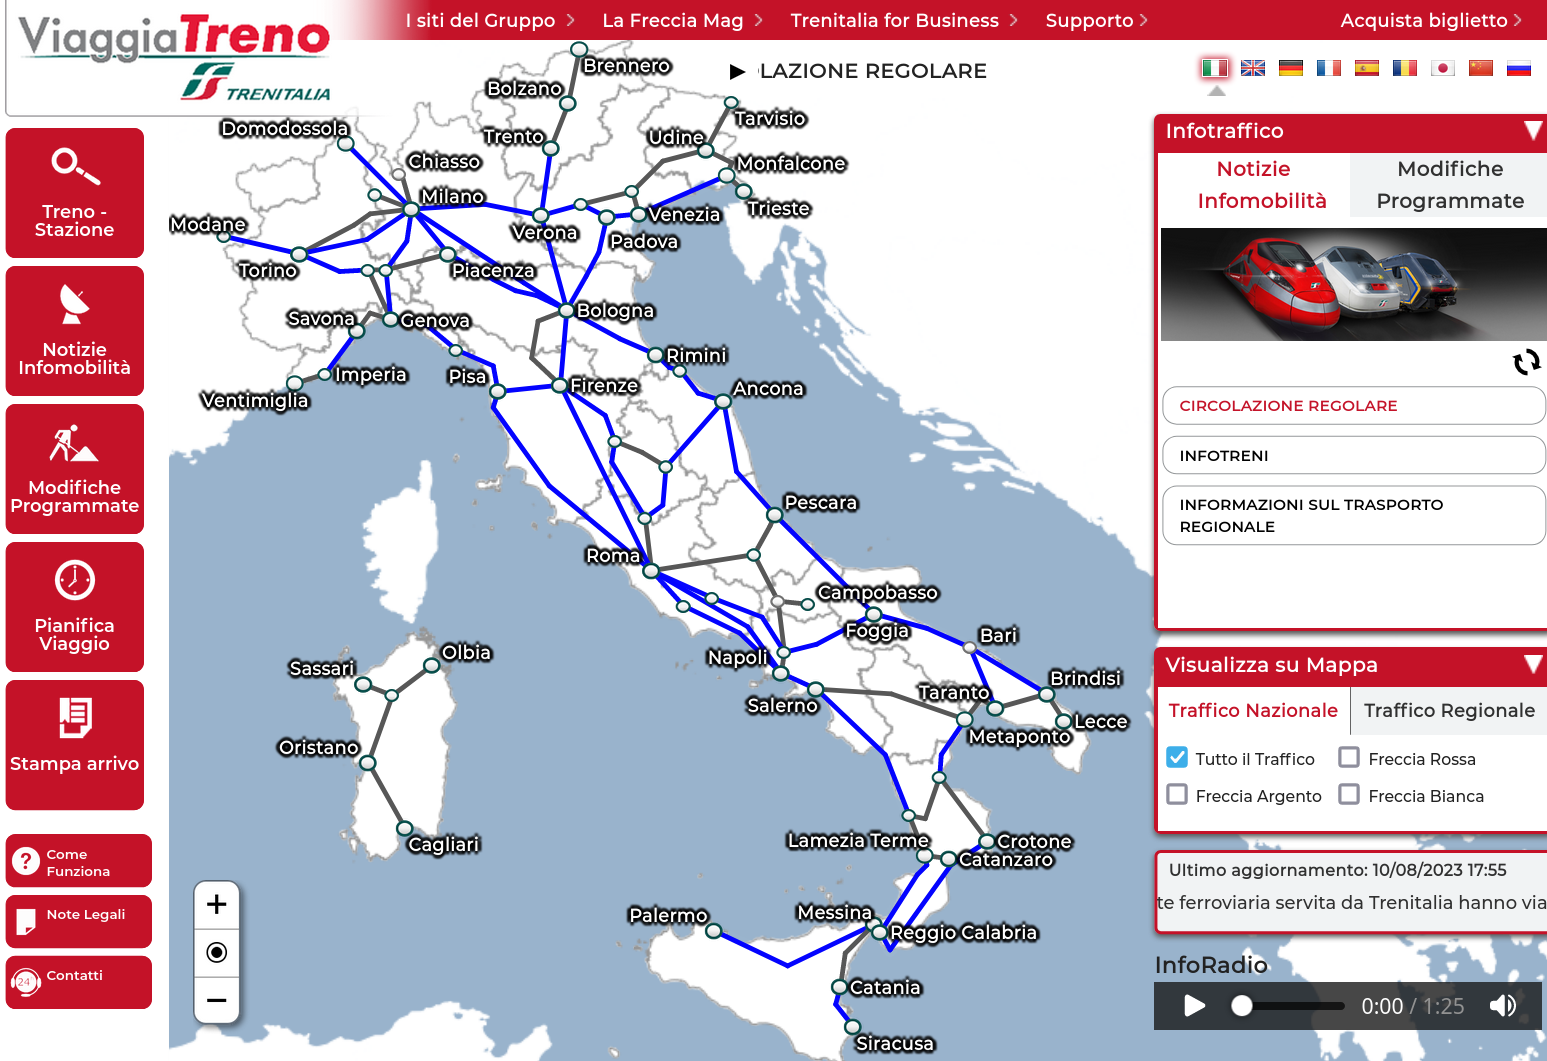
\includegraphics[width=1\textwidth]{images/viaggiatreno.png}
	\caption{Homepage di Viaggiatreno}
\end{figure}

Il portale Viaggiatreno\footnote{https://viaggiatreno.it} è stato
sviluppato da Trenitalia ed è attivo almeno dal
2006\footnote{Informazione ricavata dal \texttt{whois} del dominio}.
Il sito web permette numerose operazioni, come:
\begin{itemize}
	\item \textbf{cercare un treno} per numero o itinerario e
    visualizzare il ritardo, le fermate, luogo e orario di ultimo
    rilevamento;
	\item \textbf{cercare una stazione} per nome e visualizzare
    partenze e arrivi;
	\item \textbf{leggere o ascoltare le informazioni sulla mobilità}
    (Infomobilità).
\end{itemize}

Con Viaggiatreno è possibile trovare le corse di Trenitalia
(regionali, alta velocità, Intercity e Intercity Notte), Trenord, TPER
e OBB (Ferrovie Austriache).  \textit{Curiosamente}, non è possibile
cercare i treni di Italo-NTV, concorrente commerciale del gruppo
Ferrovie dello Stato.

La caratteristica più interessante ai fini del progetto è la
possibilità di operare anche tramite delle semplici \textbf{API HTTP},
senza autenticazione o apparenti limiti tecnologici.  Utilizzando lo
strumento \textit{``Ispeziona elemento''} di un qualsiasi browser è
possibile tracciare le richieste invocate dal frontend in JavaScript a
seguito delle azioni dell'utente e farsi un'idea dei metodi API
disponibili.

% \todo{AT: da qualche parte fare un piccolo excursus su "alla ricerca
% delle API perdute"? sui tentativi (sia tecnici che legislativi) di
% estrarre info "sensate" (4-5 stelle Berners-Lee) \\
% M: ho messo i tentativi della community in Appendice A.2}

\todo{AT: btw da qualche parte farei un microexcursus sulle
    classificazioni opendata (lo puoi riassumere dal secondo volume di
    CDT che ti posso mandare, è in fase di review ora) \\
    M: ho citato la classificazione di Berners-Lee e ho valutato gli
    ``open data'' che ho analizzato in sezione 1.3.2, va bene? \\
    AT: fai un ulteriore sforzo e usa anche quella di Davies, così li
    stronchiamo definitivamente ;) \\
    M: fatto}

\subsection{Sito web di Trenord}

\begin{figure}[h] \centering
    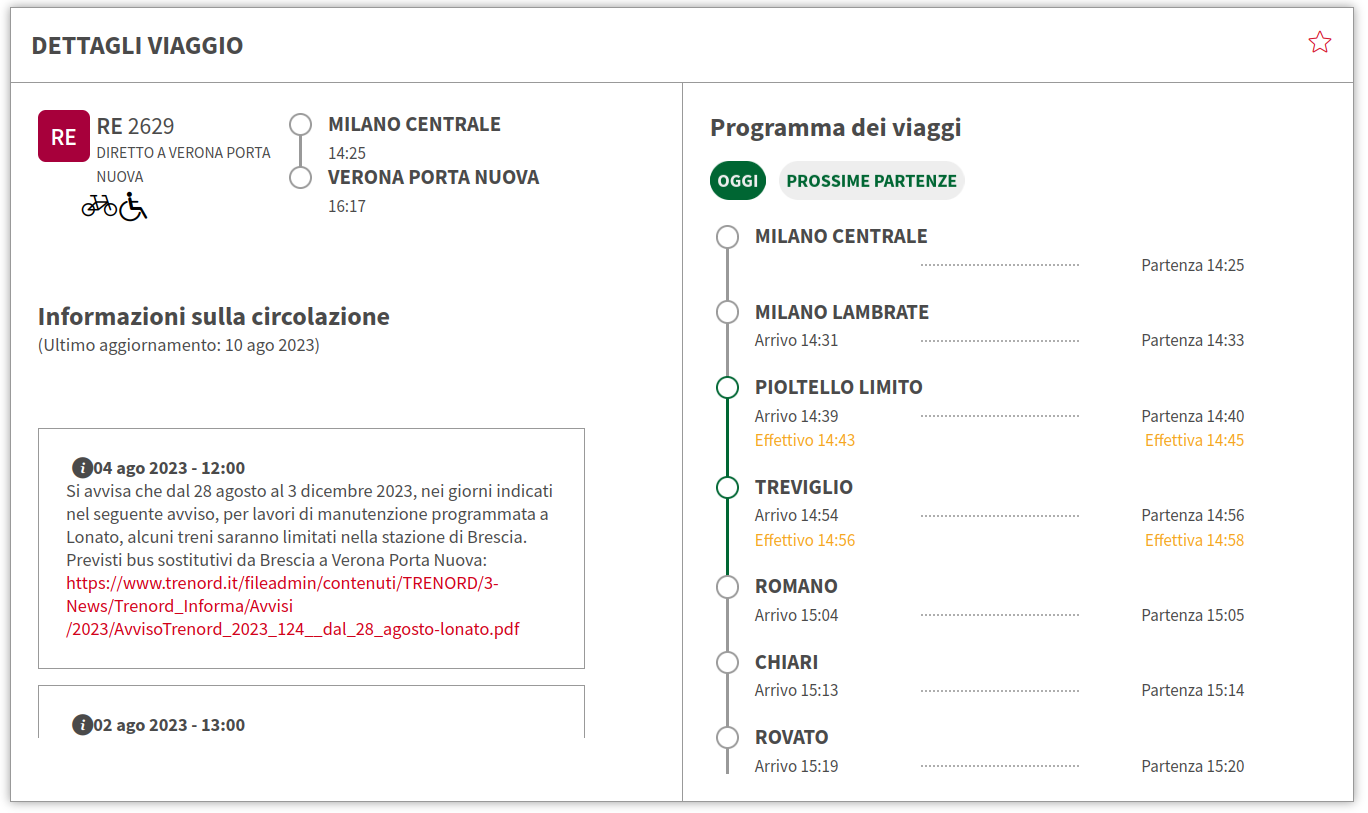
\includegraphics[width=1\textwidth]{images/trenord_api.png}
	\caption{Dettagli di una corsa sul portale web di Trenord}
\end{figure}

Trenord mette a disposizione ai viaggiatori un'applicazione mobile e
un portale web per consultare lo stato dei treni in circolazione e gli
arrivi e le partenze di una stazione.

Similmente a Viaggiatreno, con lo strumento \textit{``Ispeziona
    elemento''} si possono facilmente individuare delle \textbf{API
    HTTP} sotto la URL \texttt{https://admin.trenord.it}.  Nonostante
l'assenza di una documentazione ufficiale, l'interazione con le API
Trenord è più intuitiva e prevedibile rispetto a quelle di
Viaggiatreno.  Le risposte sono sempre in JSON e le richieste
ricalcano i principi REST di HTTP GET.

Dai portali di Trenord non si trovano corse non operate dall'impresa
stessa, come i regionali di Trenitalia o l'alta velocità.  Nonostante
ciò, le API Trenord si sono rilevate utili per verificare e correggere
alcune incongruenze riscontrate in quelle di Viaggiatreno. \\

In \S~\ref{documentazione} sono documentati alcuni metodi rilevanti
delle due API.

\section{Panorama giuridico, politico e legislativo}
\label{panorama_giuridico}

Durante il lavoro di Tesi è stato fatto ampio uso delle informazioni
fornite dalle API del portale Viaggiatreno, senza aver chiesto alcuna
autorizzazione a Trenitalia o al Gruppo Ferrovie dello Stato Italiane.
Non è però affatto scontato che i dati del trasporto \textit{pubblico}
--- come gli orari dei treni --- siano \textbf{riproducibili} e
\textbf{distribuibili} senza licenza.  Nel portale Viaggiatreno,
infatti, sono riportate le seguenti note legali (enfasi aggiunta):

\begin{quote}
	\textcquote{ViaggiatrenoToS}{I contenuti, la grafica e le immagini
        sono soggetti a Copyright. \textbf{Ogni diritto sui contenuti}
        (a titolo esemplificativo e non esaustivo: l’architettura del
        servizio, i testi, le immagini grafiche e fotografiche, ecc.)
        \textbf{è riservato ai sensi della normativa vigente}. I
        contenuti di ViaggiaTreno non possono, neppure in parte,
        essere copiati, riprodotti, trasferiti, caricati, pubblicati o
        distribuiti in qualsiasi modo senza il preventivo consenso
        scritto della società Trenitalia S.p.A. È possibile scaricare
        i contenuti nel proprio computer e/o stampare estratti
        \textbf{unicamente per utilizzo personale} di carattere
        informativo. \textbf{Qualsiasi forma di link al sito
            www.ViaggiaTreno.it deve essere preventivamente
            autorizzata} e non deve recare danno all'immagine e alle
        attività di Trenitalia S.p.A. È vietato il c.d.\ deep linking
        ossia l'utilizzo, su siti di soggetti terzi, di parti del
        Servizio Internet o, comunque, il collegamento diretto alle
        pagine senza passare per la home page del Servizio
        Internet. \textbf{L'eventuale inosservanza delle presenti
            disposizioni}, salvo esplicita autorizzazione scritta,
        \textbf{sarà perseguita} nelle competenti sedi giudiziarie
        civili e penali.}
\end{quote}

Il Gruppo Ferrovie dello Stato Italiane vieta formalmente ai soggetti
non autorizzati l’utilizzo di ViaggiaTreno per fini diversi dal mero
uso personale, riservando a sé tutti i diritti sui contenuti.  Se per
\textit{contenuti} si intendono anche le informazioni sulla
circolazione ferroviaria, allora queste \textbf{non sono utilizzabili}
senza il consenso di Trenitalia.  Non solo i dati non vengono
pubblicati, ma chi cerca di reperirli o redistribuirli rischia
\textbf{conseguenze legali}\footnote{Il lavoro di Tesi è in ogni modo
    tutelato grazie alle eccezioni alle Legge sul diritto d'autore per
    le attività di ricerca scientifica senza scopi di lucro}.
Trenitalia può farlo?

\subsection{Il caso Trenìt}
\label{caso_trenit}

Trenìt\footnote{https://trenit.app} è un'applicazione per Android e
iOS che permette di cercare e confrontare soluzioni di viaggio su
ferro tra due stazioni.  La sua \textbf{semplicità} e \textbf{facilità
    d'uso} hanno contribuito al suo notevole successo.  Oltre agli
orari e allo stato attuale dei treni, vengono mostrati i
\textbf{prezzi} dei biglietti rendendo possibile \textbf{comparare} le
offerte commerciali delle imprese ferroviare.

Il 19 luglio 2019 Trenìt è stata costretta a \textbf{sospendere il
    servizio} \cite{TrenitSospensione, TrenitFQ, TrenitWired} a causa
di un provvedimento cautelare emesso dal Tribunale di Roma sotto
ricorso di Trenitalia.

\begin{quote}
    \textcquote[Nota di Trenìt]{TrenitSospensione}{Purtroppo dobbiamo
        sospendere temporaneamente il servizio, perché
        \textbf{Trenitalia non vuole che pubblichiamo i dati}
        (pubblici) relativi ai suoi treni e quindi ci ha fatto causa,
        ritenendo che l’uso che facciamo dei suoi dati sia illegittimo
        in quanto non autorizzato. Noi, invece, siamo convinti che il
        nostro operato sia pienamente lecito e non arrechi alcun danno
        agli operatori ferroviari. Al contrario, pensiamo che il
        nostro uso dei dati pubblici relativi al trasporto ferroviario
        arrechi un vantaggio agli operatori (visto che promuove i loro
        servizi).}
\end{quote}

Trenitalia d'altro canto lamentava, oltre all'uso dei dati senza
autorizzazione, un \textbf{carico esoso per i propri server} causato
dall'attività di \textit{scraping}\footnote{Scaricamento automatizzato
    di informazioni da interfacce utente} e una \textbf{comparazione
    imparziale} delle offerte commerciali.  Di seguito è riportato il
suo commento a \textit{Wired}.

\begin{quote}
    \textcquote[Nota di Trenitalia]{TrenitWired}{Nessun ostacolo alla
        sharing economy.  Trenitalia, come è stato dimostrato in altre
        occasioni, è aperta alla condivisione delle informazioni, a
        patto che ciò avvenga rispettando regole certe e ben definite.

        Trenìt! estraeva e diffondeva, senza alcun accordo, dati
        ottenuti interrogando il sistema di vendita di Trenitalia.
        Ciò costituisce una violazione della disciplina vigente che
        vieta a terzi non autorizzati di reimpiegare a scopo di lucro
        informazioni, soprattutto se di natura commerciale.}
\end{quote}

Trenitalia, almeno in pubblico, \textbf{non si è dimostrata aperta}
alla condivisione delle informazioni.  I termini di servizio di
Viaggiatreno \cite{ViaggiatrenoToS} non permettono nessun uso diverso
da quello strettamente personale.

\begin{quote}
    \textcquote[Nota di Trenitalia,
    \textit{cont.}]{TrenitWired}{Inoltre, presentando un incompleto
        pacchetto di offerte di Trenitalia, l’app non offriva al
        cliente un confronto equilibrato.  Tema che, in un settore a
        mercato, è fondamentale per garantire ad ogni viaggiatore la
        possibilità di scegliere, con consapevolezza, fra tutte le
        opzioni di viaggio disponibili.}
\end{quote}

In sede di giustizio non sono risultate evidenze di
\textbf{distorsioni} del confronto tra le offerte di Trenitalia e
della sua concorrenza.  Si può invece rilevare l'assenza
dell'\textbf{offerta della concorrenza} su Viaggiatreno e sull'app di
Trenitalia: a differenza dei servizi di terze parti, le imprese
ferroviarie non sembrano interessate a proporre una piattaforma unica
per l'acquisto di biglietti ferroviari.

\begin{quote}
    \textcquote[Nota di Trenitalia, \textit{cont.}]{TrenitWired}{I
        dati relativi alle offerte commerciali di Trenitalia sono
        stati acquisiti da Trenìt! attraverso continue, perduranti e
        massive interrogazioni del sistema Trenitalia: ogni giorno
        circa 800mila richieste, con picchi che hanno superato le
        14mila richieste ogni 10 minuti.  Sistema di vendita la cui
        realizzazione è stata sostenuta da Trenitalia grazie a
        consistenti investimenti.

        La posizione di Trenitalia è stata al momento riconosciuta
        fondata dal Tribunale di Roma.}
\end{quote}

È stato riconosciuto in giudizio che \textcquote{TrenitSentenza}{il
    numero aritmetico degli accessi riscontrati da Trenitalia si pone
    poi in logico contrasto con un sistematico download dei dati da
    parte dei server della società GoBright Media Ltd (\textit{Trenìt,
        n.d.r.}), la quale non avrebbe bisogno di effettuare un così
    alto e capillare numero di accessi se procedesse al
    \textbf{download sistematico} dei dati Trenitalia sui propri
    server}.  Se Trenìt non esistesse è ragionevole supporre che la
\textit{domanda di informazione} sarebbe comunque soddisfatta da
Trenitalia stessa, trovandosi in condizione di \textbf{monopolio}
nell'\textbf{accesso delle informazioni}.

\subsubsection{La sentenza}

Il 5 settembre dello stesso anno, il Tribunale di Roma \textbf{revoca}
il provvedimento cautelare emesso in precedenza \cite{TrenitSentenza}:
\textbf{Trenìt può continuare ad operare}.  Secondo il giudice, Trenìt
ha estratto una \textquote{\textbf{parte non sostanziale}} del
contenuto della banca dati.  Secondo l'art.\ 102 ter
LDA\footnote{Legge sul diritto d'autore}, infatti,
\textquote{\textbf{non sono soggette all'autorizzazione} del
    costitutore della banca dati \textbf{messa per qualsiasi motivo a
        disposizione del pubblico} le attività di estrazione o
    reimpiego di \textbf{parti non sostanziali} valutate in termini
    qualitativi e quantitativi del contenuto della banca dati per
    qualsivoglia fine effettuate dall'utente legittimo}.

Trenitalia ad oggi non ha presentato ulteriori ricorsi.

\subsubsection{Osservazioni}

Carlo Piana, noto avvocato italiano attivo nel campo del software
libero, ha pubblicato delle osservazioni su alcuni punti della
sentenza nel suo articolo ``\textit{Scraping di dati pubblici per non
    perdere il treno della concorrenza}'' \cite{TrenitPiana} per
TechEconomy2030.

Nel 2010 LastMinute e Ryanair sono andati in causa perché la prima
offriva al pubblico uno \textbf{strumento di comparazione dei prezzi}
con i dati della seconda.  La sentenza \cite{RyanairSentenza} del
Tribunale di Milano richiama un concetto interessante della
legislazione sulla tutela giuridica delle banche dati:
\textcquote[considerando 47]{Dir9}{\textit{considerando che, al fine
        di favorire la concorrenza fra i fornitori di prodotti e
        servizi nel settore del mercato dell'informazione, \textbf{la
            protezione sulla base del diritto «sui
            generis»\footnote{Il diritto che tutela giuridicamente il
                contenuto di una banca dati} non deve essere
            esercitata in modo tale da favorire gli abusi di posizione
            dominante}, con particolare riguardo alla creazione e
        diffusione di nuovi prodotti e servizi a valore aggiunto di
        ordine intellettuale, documentale, tecnico, economico o
        commerciale; che, pertanto, le disposizioni della presente
        direttiva lasciano impregiudicata l'applicazione delle regole
        di concorrenza, siano esse comunitarie o nazionali}}.  La
\textbf{posizione dominante} di Trenitalia nel mercato della fornitura
dei dati della circolazione ferroviaria è quindi probabilmente
\textbf{incompatibile} con l'esercizio del diritto sui generis.

Secondo Piana, infine, non è scontato che la banca dati in oggetto
\textit{sia una banca dati} proteggibile tramite il diritto sui
generis.  Il diritto del costitutore di vietare operazioni di
estrazione di una parte sostanziale della banca dati è garantito solo
qualora \textcquote[art.\ 7]{Dir9}{\textit{\textbf{il conseguimento,
            la verifica o la presentazione di tale contenuto attestino
            un investimento rilevante} sotto il profilo qualitativo o
        quantitativo}}.  Si può quindi argomentare che gli
\textit{investimenti rilevanti} di Ryanair e Trenitalia nella
creazione delle rispettive piattaforme siano finalizzati all'esercizio
del \textbf{servizio di prenotazione} e \textbf{assistenza alla
    clientela} e non alla \textit{presentazione} della banca dati.
Secondo questa interpretazione \textit{i dati sono un mezzo} e non uno
scopo, pertanto non può essere vantato diritto sui generis.

\subsection{Ferrovie italiane e Open Data: due binari paralleli?}

È irragionevole \textbf{pretendere} che i dati \textit{pubblici}, di
imprese \textit{pubbliche}, operatrici di servizio \textit{pubblico}
con fondi \textit{pubblici} siano
\textbf{\textit{aperti}}\footnote{Secondo AgID \cite{AgidOpenData}, un
    \textbf{dato} si dice ``\textbf{aperto}'' quando è rilasciato con
    una licenza o normativa che ne permetta l'\textbf{utilizzo
        libero}, è \textbf{accessibile con tecnologie digitali} ed è
    \textbf{reso disponibile gratuitamente} o a costi marginali}?
Secondo l'autore di questa Tesi, il Cittadino dovrebbe aver diritto di
\textbf{accedere liberamente} ai dati della circolazione ferroviaria,
scegliere l'\textit{app} che ritiene più adatta o svilupparne una
propria, senza limitazioni o autorizzazioni.  Dovrebbe essere anche
garantita la libertà di poter analizzare i \textit{dataset} storici
per misurare e calcolare la \textbf{performance} reale.  Come si può
iniziare un dialogo sul trasporto pubblico senza l'accesso ai dati?

\subsubsection{Classificazione degli Open Data}

Tim Berners-Lee ha proposto \cite{W3LinkedData} uno schema di
\textbf{classificazione} degli \textit{open data} basato su 5 stelle:
\begin{itemize}
    \item $\star$: è disponibile su Internet ed è distribuito con una
    \textbf{licenza libera};
    \item $\star\,\star$: è \textbf{\textit{machine-readable}};
    \item $\star \star \star$: è distribuito in un \textbf{formato non
        proprietario};
    \item $\star \star \star\,\star$: usa gli
    \textbf{URI}\footnote{\textit{Unique Resource Identifier},
        identificatore univoco di una risorsa} per identificare gli
    oggetti;
    \item $\star \star \star \star \star$: \textbf{si collega} ad
    altri dati per fornire il contesto.
\end{itemize}

Un'altra proposta, avanzata da Tim Davies~\cite{DaviesOpenData},
valuta gli \textbf{aspetti più \textit{umani}}:

\begin{itemize}
    \item $\star$ (\textit{be demand driven}): le scelte su quali dati
    rilasciare, la loro struttura e gli strumenti sono guidate dalla
    domanda della comunità e dall'utilità effettiva;
    \item $\star\,\star$ (\textit{put data in context}): sono fornite
    informazioni chiare su \textit{quali} dati sono disponibili,
    inclusa la frequenza degli aggiornamenti, i formati e la qualità;
    \item $\star \star \star$ (\textit{support conversation around
        data}): la comunità può partecipare commentando e avanzando
    proposte, anche offline e in modo strutturato;
    \item $\star \star \star\,\star$ (\textit{build capacity, skills
        and networks}): sono forniti strumenti, guide e aiuto a coloro
    che desiderano interpretare ed utilizzare i dati;
    \item $\star \star \star \star \star$ (\textit{collaborate on data
        as a common resource}): sono in essere processi e meccanismi
    per permettere alla community di migliorare i \textit{dataset} e
    creare nuove risorse basate su quanto già pubblicato.
\end{itemize}

Nella prossima sezione verranno illustrati e valutati alcuni dati
pubblicati dagli Enti titolari di contratto di servizio con le imprese
ferroviarie.

\subsubsection{Monitoraggio nei contratti di servizio}

Nella totalità dei contratti di servizio esaminati (vedi
\S~\ref{servizio_pubblico}) sono presenti accordi di \textbf{verifica}
e \textbf{monitoraggio} dell'operato delle imprese ferroviarie, che
devono corrispondere agli Enti committenti \textbf{penali} in base ad
alcune \textbf{metriche di puntualità} e \textbf{affidabilità}.
Confrontare le metriche di Enti o imprese diverse è spesso
\textbf{impossibile}: nonostante le formule RFI della
\textit{performance regime} (vedi \S~\ref{performance_regime}) siano
spesso utilizzate come base di partenza, ogni contratto è diverso.
L'accesso ai c.d.\ ``\textit{dati elementari di base}'' (le
rilevazioni grezze) è spesso garantito solo all'Ente committente, non
al Cittadino.  Le metriche sono spesso pubblicate in \textbf{modalità
    aggregata}, o non pubblicate affatto.  I Cittadini sono gli
\textbf{stakeholder principali} del servizio, che in quanto
\textbf{pubblico} dovrebbe favorire attività di
\textbf{\textit{citizen science}}\footnote{Con \textit{citizen
        science}, o \textit{scienza dei cittadini}, si intendono le
    attività di ricerca scientifica amatoriale portate avanti da
    cittadini} da parte degli stessi.

\paragraph{Lombardia}

\begin{figure}[h] \centering
    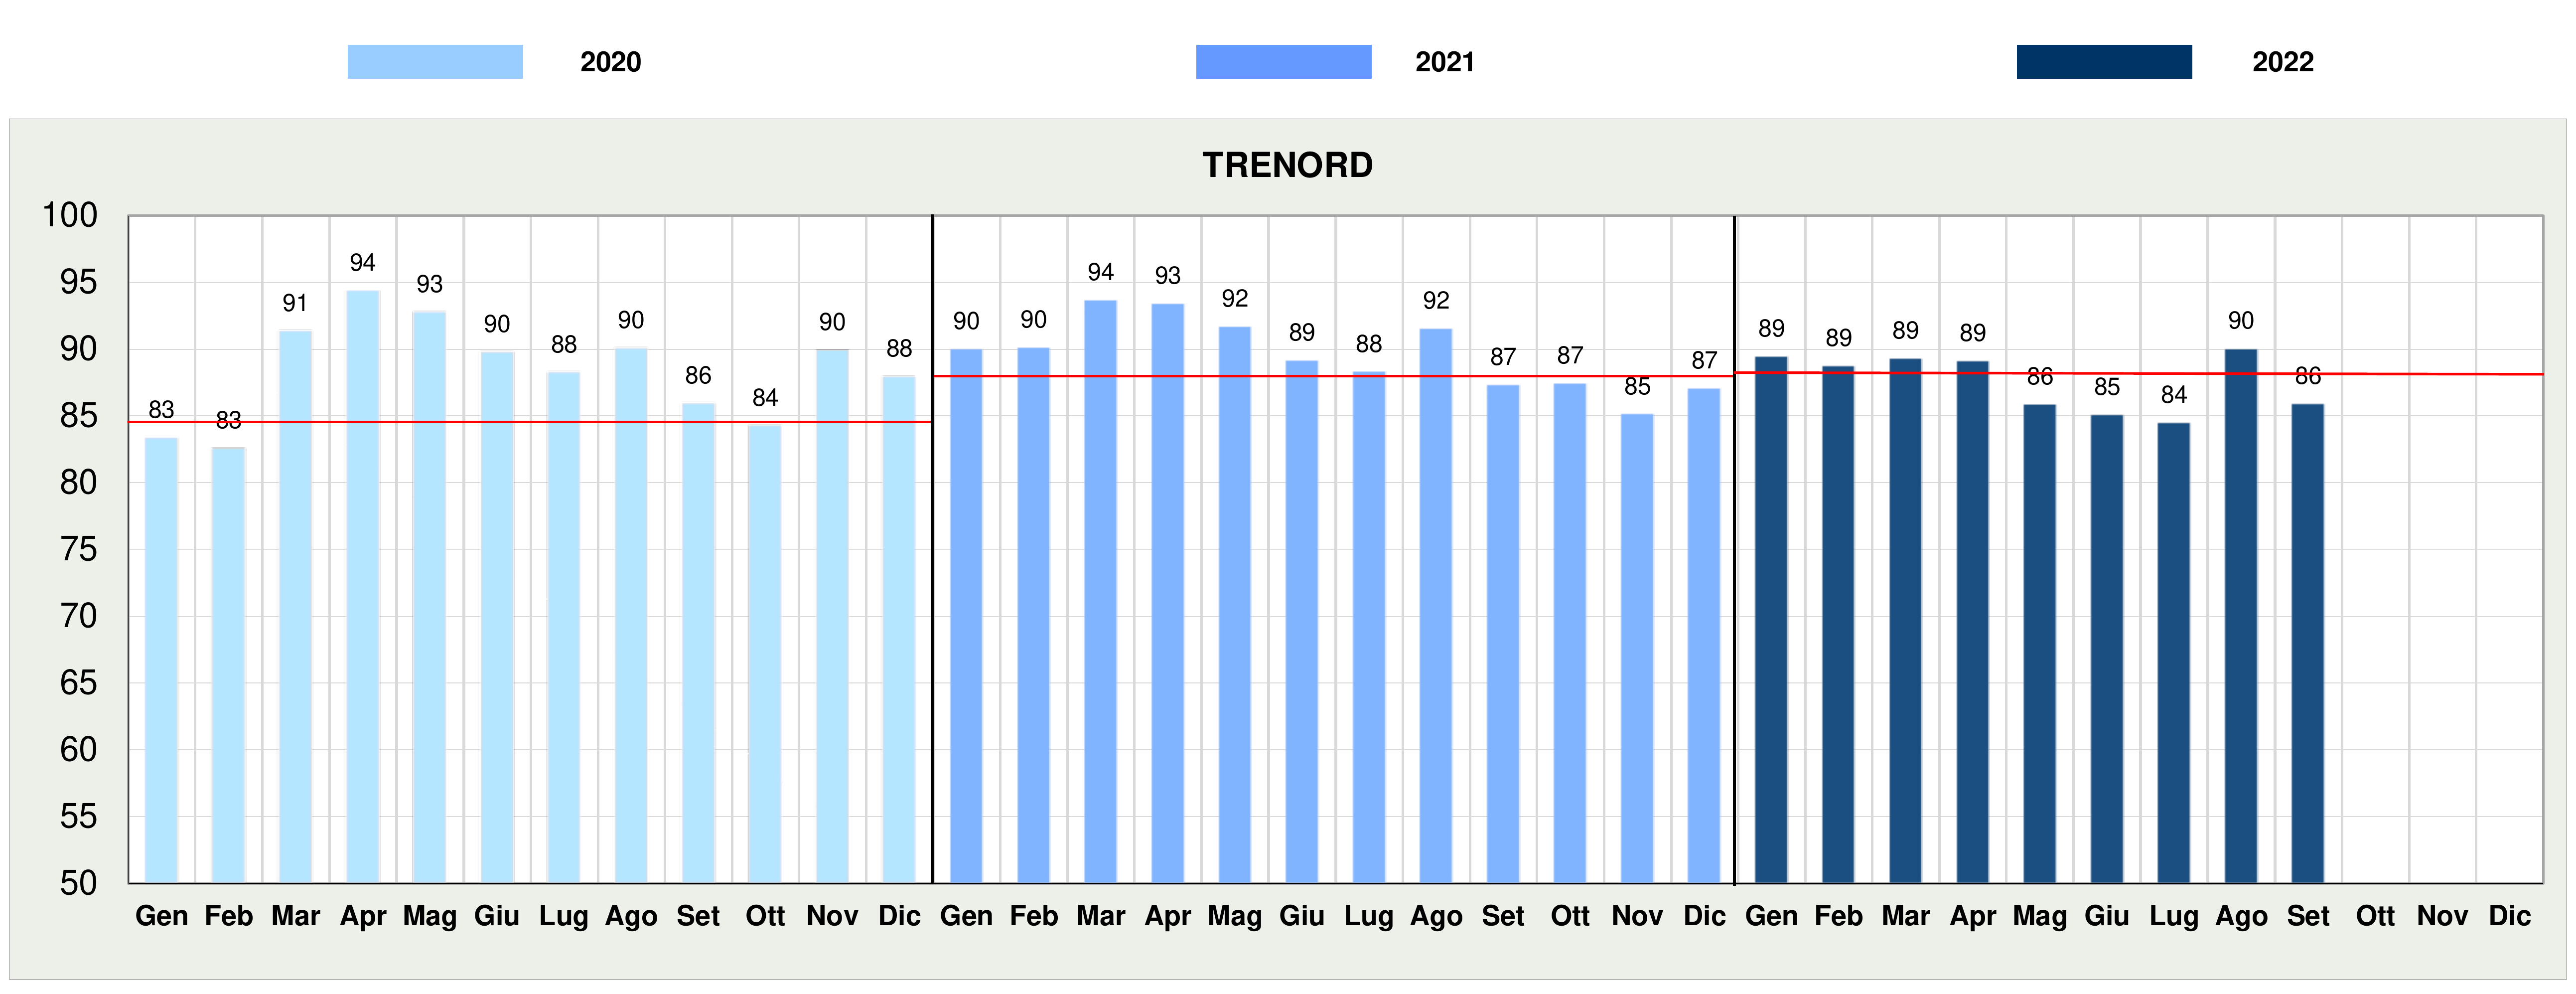
\includegraphics[width=1\textwidth]{images/lombardia_puntualita.png}
	\caption{Dati ufficiali sulla puntualità dei treni in Lombardia
        \cite{LombardiaDati}}
    \label{lombardia_puntualita}
\end{figure}

\begin{figure}[h] \centering
    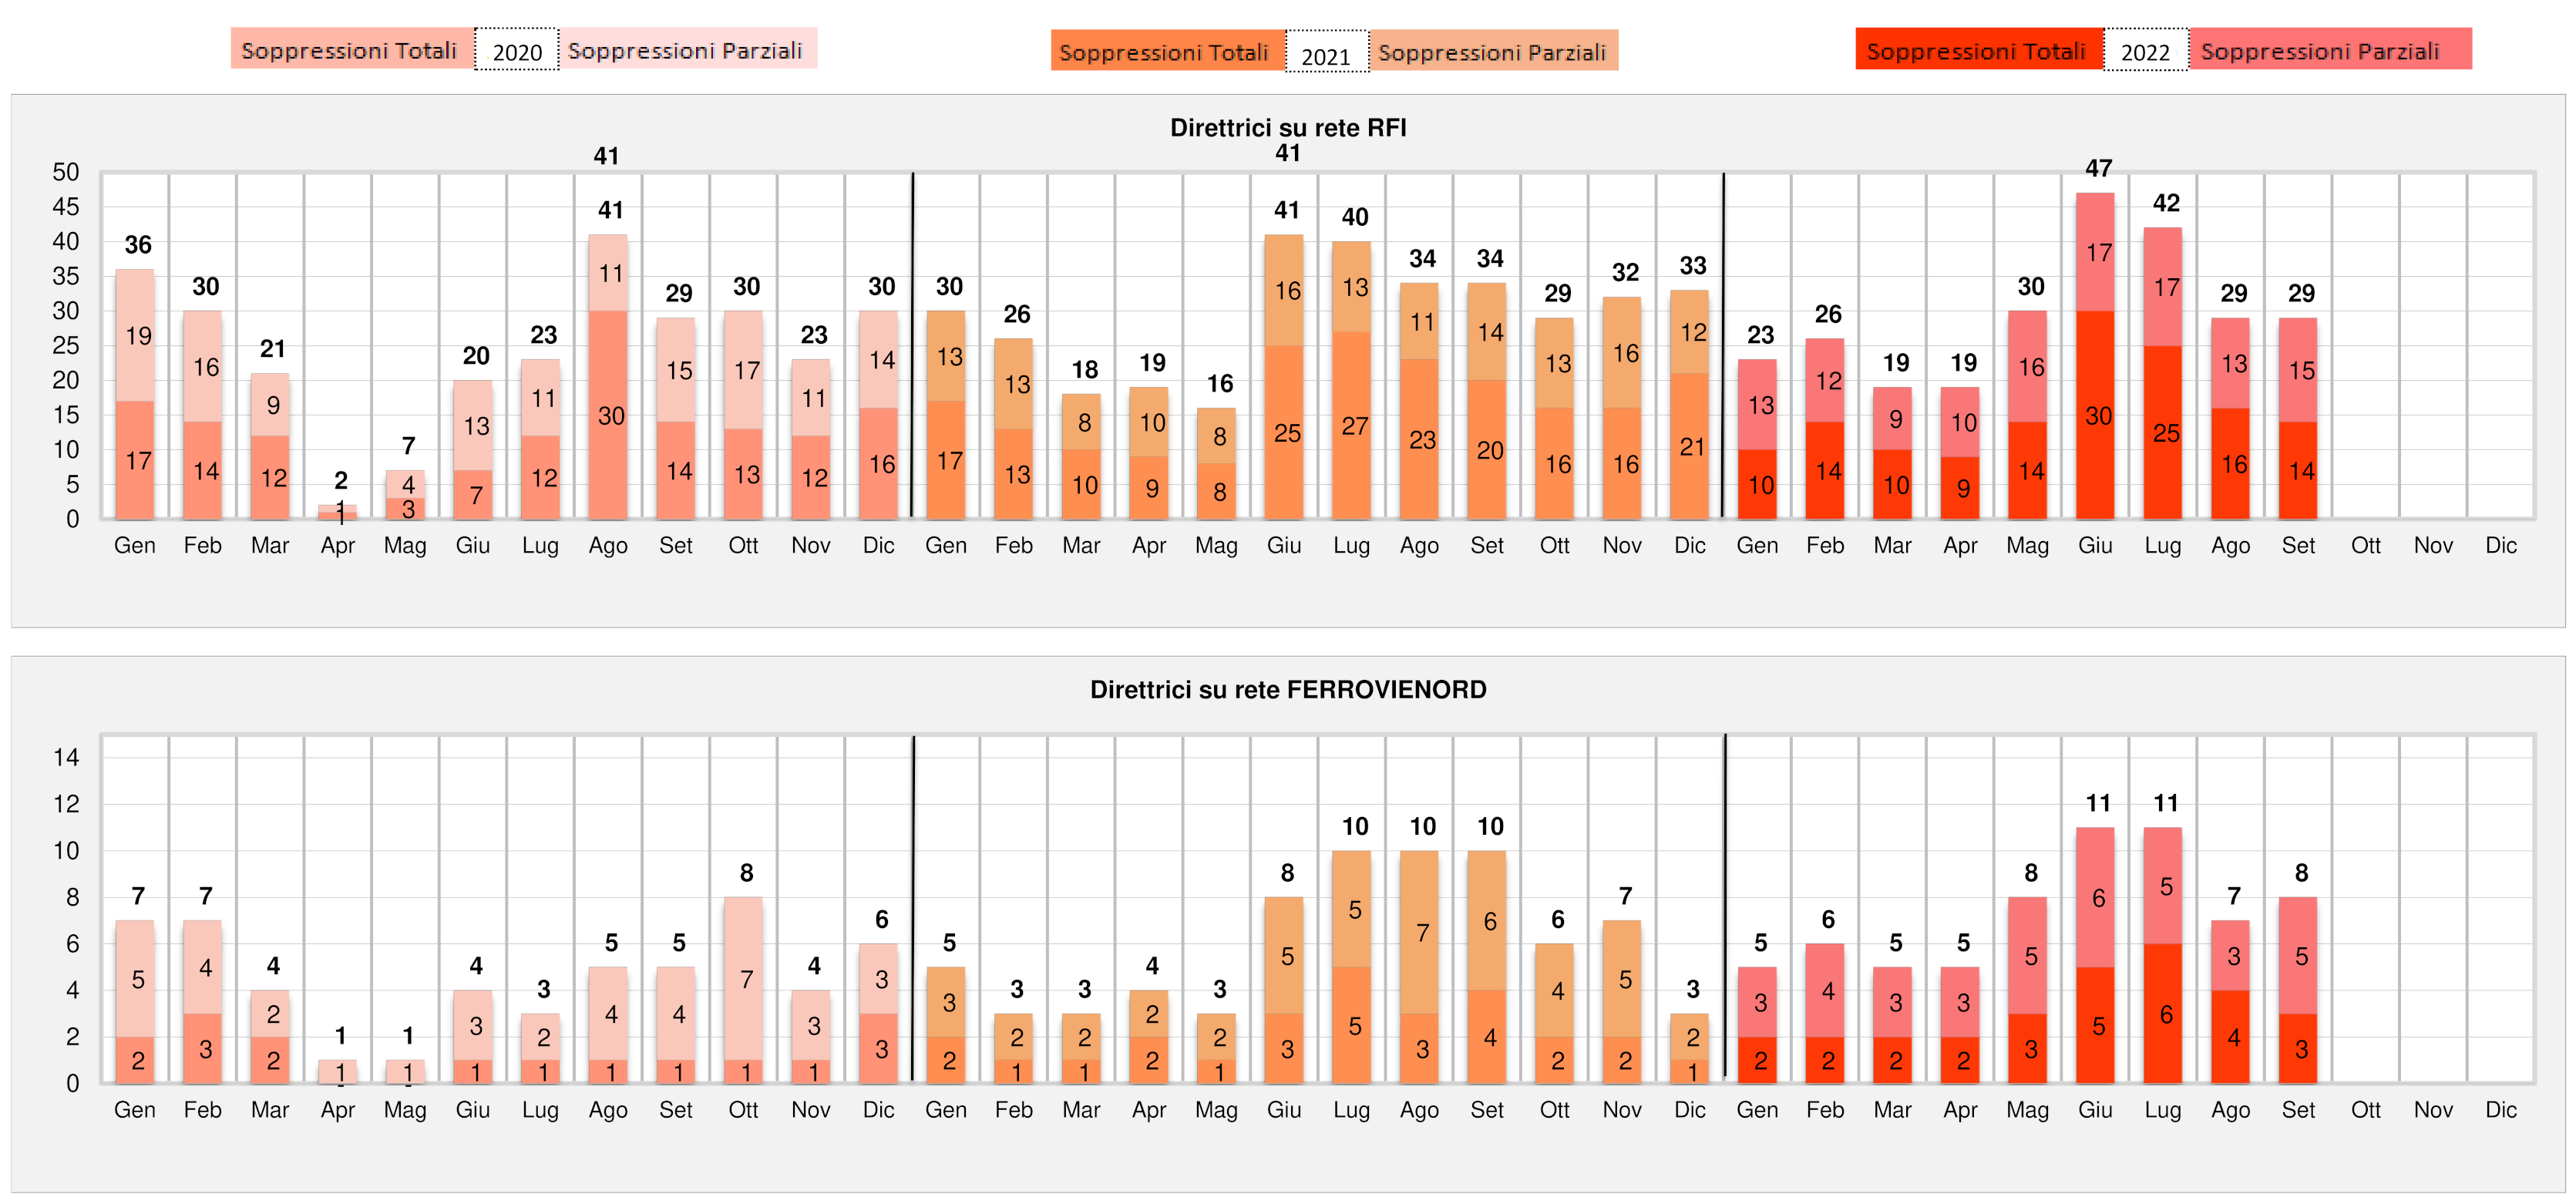
\includegraphics[width=\linewidth]{images/lombardia_affidabilita.png}
    \caption{Dati ufficiali sulla affidabilità dei treni in Lombardia,
        raggruppati per gestore dell'infrastruttura
        \cite{LombardiaDati}}
    \label{lombardia_affidabilita}
\end{figure}

Per esempio, Regione Lombardia pubblica sul proprio sito istituzionale
\cite{LombardiaDati} l'\textbf{indice di puntualità}, inteso come la
\textquote{\textit{percentuale di corse giunte a destino\footnote{Nel
            gergo ferroviario, la destinazione finale} entro 5 minuti
        per media intera giornata\footnote{Escludendo
            \textquote{\textit{cause di forza maggiore, scioperi e
                    lavori programmati}}\label{forza_maggiore}}}} e
l'\textbf{indice di affidabilità}, ovvero il \textquote{\textit{numero
        medio di corse soppresse al giorno per tutto il percorso o
        parzialmente\footnote{Vedi la nota
            \footref{forza_maggiore}}}}.  Per entrambe le metriche i
dati sono presentati \textbf{aggregati} per mese e per gestore
dell'infrastruttura (vedi \figurename~\ref{lombardia_puntualita}
e~\ref{lombardia_affidabilita}), rendendo impossibile confrontare
direttrici, orari, giorni della settimana o imprese ferroviarie.  Gli
\textbf{indici} stessi sono \textbf{fuorvianti}: due treni che
arrivano a destino con 6 e 60 minuti di ritardo sono conteggiati
ugualmente, mentre le fermate intermedie non vengono considerate.  Il
\textbf{numero assoluto} di \textit{corse soppresse al giorno} è un
\textbf{dato poco significativo} senza il numero di corse complessivo.
Le \textbf{responsabilità tra le parti} delle perturbazioni al
servizio \textbf{non sono \textit{rivelate}}, nonostante siano
certamente state \textit{rilevate} ai fini di contratto di servizio e
\textit{performance regime}.  Infine, il formato PDF non li rende
facilmente analizzabili meccanicamente e i dati \textbf{non sono
    aggiornati} da più di 11 mesi risultando poco utili al pubblico:
sono quindi rispettivamente valutati con \textbf{1 stella} ($\star$) e
\textbf{0 stelle} secondo la classificazioni proposte da Tim
Berners-Lee e Tim Davies.

\paragraph{Emilia-Romagna}
Un panorama diverso si presenta in Emilia-Romagna, dove FER (gestore
dell'infrastruttura) è incaricata di pubblicare in dettaglio le
\textbf{singole corse} giunte a destino in ritardo o cancellate,
specificando anche \textbf{responsabilità} e \textbf{motivazioni}
\cite{FerDati}.  I treni sono raggruppabili per \textbf{tipo di
    evento} (ritardo o soppressione), \textbf{direttrice} e
\textbf{rete} (RFI o FER) (vedi \figurename~\ref{fer_dati}).  I dati
sono presentati con un'\textbf{interfaccia semplice} e
\textbf{intuitiva} e sono addirittura esportabili in \textbf{CSV}.
Regione Emilia-Romagna ha dimostrato che la \textbf{trasparenza} in
questo campo è possibile, anche se sul portale non sono indicate le
\textbf{fermate intermedie} e i \textbf{treni regolari}: per analisi
più approfondite tali dati potrebbero risultare utili.

\textbf{Aldo Salani}, responsabile dell'Area Commerciale FER e
interpellato via posta elettronica durante il lavoro di Tesi,
rivela\footnote{Nelle citazioni che seguono, le enfasi sono aggiunte}
che \textcquote{Salani}{FER non solo ha a disposizione la
    \textbf{propria banca dati} di programmazione, gestione e
    contabilizzazione dei dati di circolazione, ma ha anche accesso a
    quella del gestore nazionale tramite i sistemi dell'impresa
    ferroviaria che espleta il servizio; ciò consente, attraverso un
    sistema di \textbf{gestione big data}, di elaborare un cruscotto
    informatico che gestisce e mostra i dati autonomamente con
    \textbf{precisione} e \textbf{profondità}, evitando di ricevere
    prospetti preconfezionati e poco versatili.  Tra l'altro oltre al
    monitoraggio della puntualità e della regolarità (soppressioni),
    il cruscotto mostra anche i \textbf{dati della qualità erogata},
    dati che vengono raccolti da una \textbf{squadra di ispettori} che
    giornalmente svolge turni sui treni inserendo in tempo reale a
    sistema elementi quali illuminazione, riscaldamento,
    condizionamento, pulizia, stato dei servizi igienici,
    comportamento del personale ecc..}.  Perché le \textbf{altre
    Regioni} non sono così trasparenti?  \textcquote{Salani}{Il
    modello FER è attualmente difficilmente applicabile alle altre
    regioni per il fatto che in questo caso la Regione ha scelto di
    affidare lo svolgimento della \textbf{gara per il trasporto
        pubblico} su rotaia e la successiva gestione del relativo
    contratto di servizio alla \textbf{società in house} FER che è il
    gestore infrastruttura della rete ferroviaria regionale}.  Salani
si è dimostrato aperto ai miglioramenti del portale e precisa che
\textcquote{Salani}{il lasso di tempo, a volte un po' lungo,
    necessario per la pubblicazione dipende da quando i gestori
    infrastruttura comunicano il \textbf{``consolidamento''} dei dati
    i quali possono subire variazioni in seguito a revisioni
    successive (soprattutto in merito alle cause dei ritardi)}.

L'uso di formati liberi e \textit{machine-readable} premia i dati
messi a disposizione da Regione Emilia-Romagna con \textbf{3 stelle}
($\star \star \star$) secondo la classificazione di Tim Berners-Lee ma
solamente \textbf{2 stelle} ($\star\,\star$) di Tim Davies, in quanto
alla communità manca la possibilità di commentare e interagire.

\begin{figure}[h] \centering
    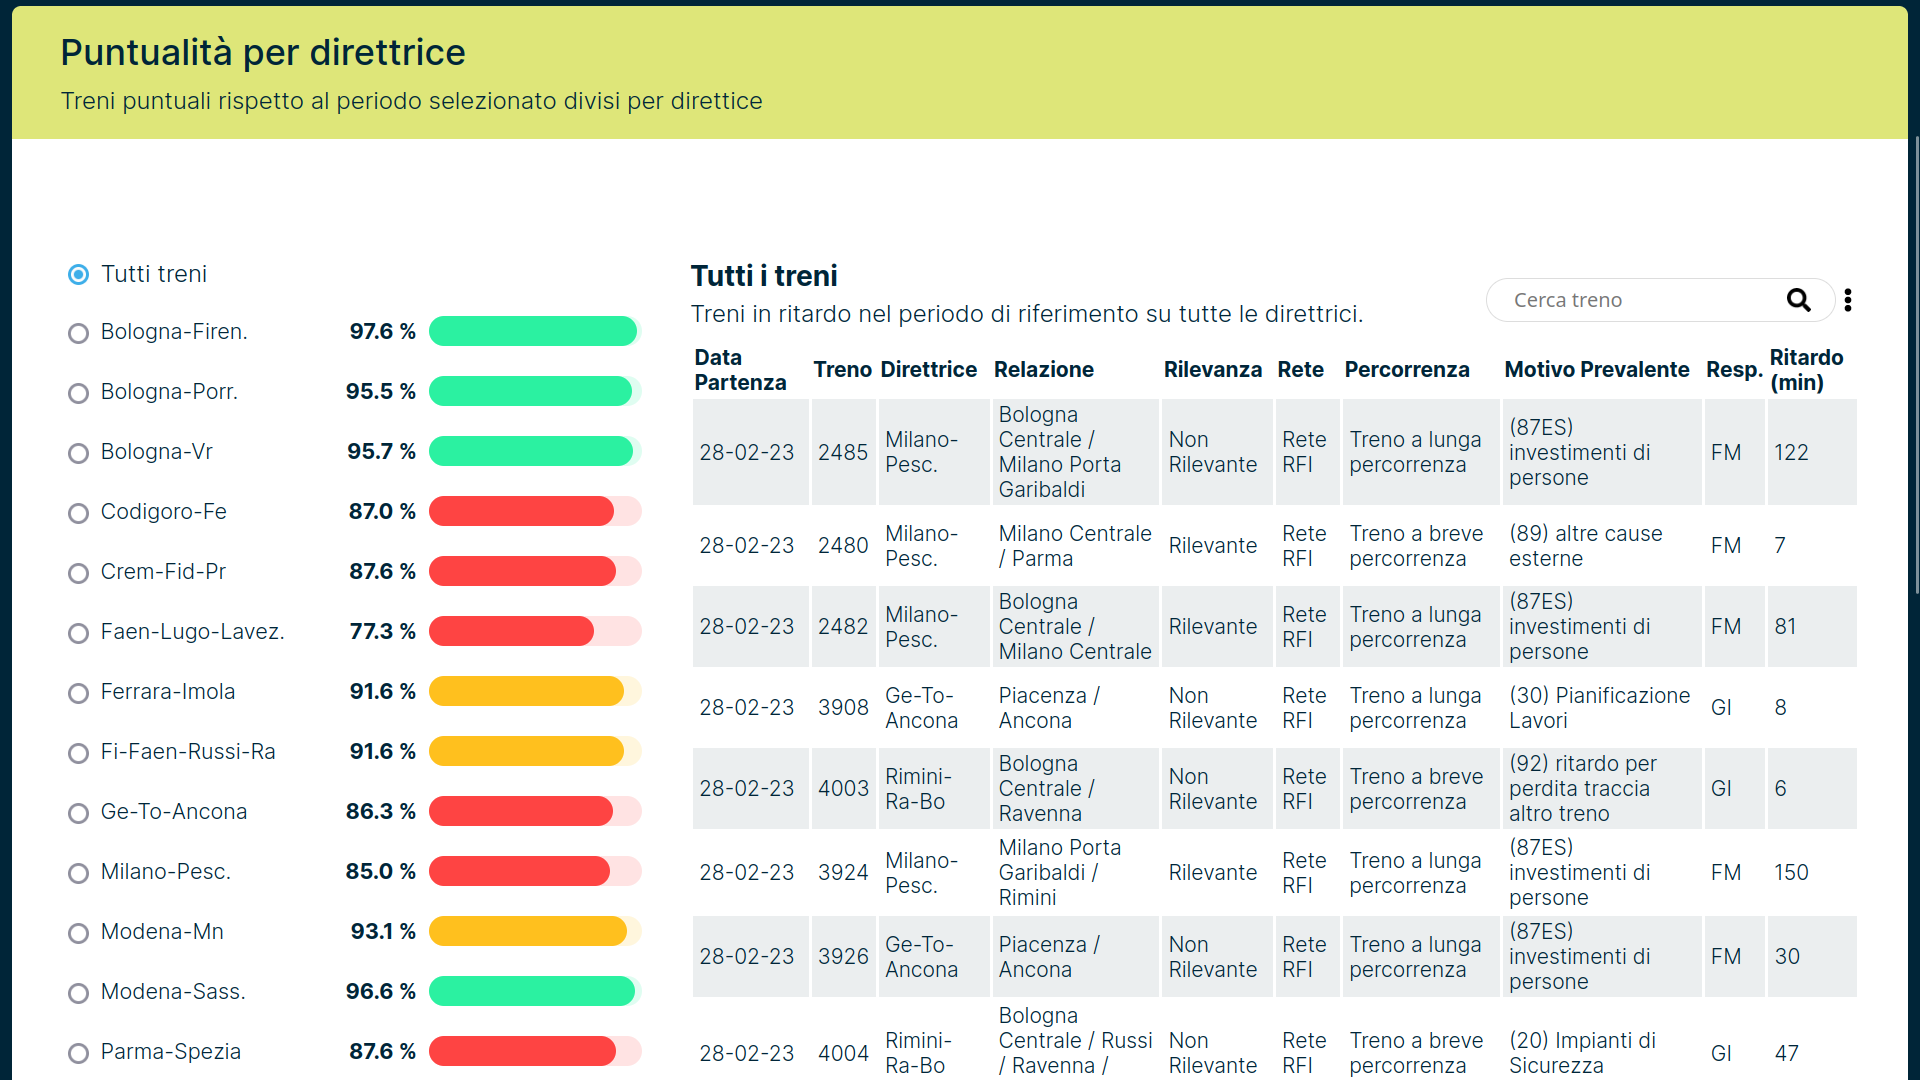
\includegraphics[width=1\textwidth]{images/fer_dati.png}
	\caption{Dati ufficiali sulla puntualità dei treni in Emilia
        Romagna \cite{FerDati}}
    \label{fer_dati}
\end{figure}


\subsection{Accesso civico generalizzato}
\label{foia}

Dopo lunghe battaglie di cittadinanza attiva da parte di gruppi come
Foia4Italy \cite{SilenziDiStato}, nel 2016 il ``decreto Trasparenza''
\cite{Dlgs97} introduce il \textbf{Foia}\footnote{Dagli USA,
    \textit{Freedom of Information Act}} in Italia.  Secondo la
normativa, \textcquote[art.\ 5]{Dlgs33}{\textit{allo scopo di favorire
        forme diffuse di controllo sul perseguimento delle funzioni
        istituzionali e sull'utilizzo delle risorse pubbliche e di
        promuovere la partecipazione al dibattito pubblico,
        \textbf{chiunque ha diritto di accedere} ai dati e ai
        documenti detenuti dalle pubbliche amministrazioni}}.
L'accesso è regolato presentando un'\textbf{istanza di accesso civico
    generalizzato}: l'Amministrazione deve tassativamente rispondere
entro \textbf{30 giorni} con la trasmissione dei documenti richiesti o
con un diniego adeguatamente motivato.

Durante il lavoro di Tesi sono state inoltrate a fini esplorativi due
richieste di \textbf{accesso civico generalizzato} per i dati citati
nei contratti di servizio, illustrati qui di seguito.

\subsubsection{Ministero delle Infrastrutture e dei Trasporti per
    Trenitalia}

Il contratto di servizio tra il \textbf{MIT} e \textbf{Trenitalia}
riguarda principalmente i treni a media e lunga percorrenza in regime
di \textbf{servizio pubblico}, ovvero gli \textit{intercity} e
\textit{intercity notte}.  L'oggetto principale della richiesta
riguardava i dati di monitoraggio descritti nell'Allegato 6
\cite[art.\ 5, comma 1, lettera g]{CdSMIT}, ovvero le rilevazioni in
formato tabellare \textbf{per ogni singolo treno} di
\textbf{puntualità}, \textbf{frequentazione}, \textbf{pulizia}, e
\textbf{tasso di riempimento}.

La risposta del Ministero è stata un \textbf{diniego}, giustificato
dalla \textcquote{FoiaMIT}{possibilità di un pregiudizio concreto alla
    tutela [...] degli interessi economici e commerciali} di
Trenitalia, in qualità di \textbf{soggetto
    controinteressato}\footnote{La normativa sul Foia \cite{Dlgs33}
    stabilisce criteri precisi per identificare i soggetti
    controinteressati e ammette il diniego in caso la pubblicazione
    dei documenti oggetto dell richiesta possa pregiudicare interessi
    privati, tra cui interessi economici}.  Di seguito è riportata
integralmente la motivata opposizione dell'Azienda.

\begin{quote}
    \textcquote{FoiaMIT}{\textbf{I dati/la documentazione richiesta
            hanno tutt’oggi carattere di assoluta riservatezza}, in
        quanto attinenti ad informazioni di natura commerciale,
        industriale ed economico finanziaria la cui indebita
        diffusione recherebbe un \textbf{grave e concreto pregiudizio
            a Trenitalia}, anche per il grado di analiticità in cui
        gli stessi sono articolati.  Nello specifico, si rappresenta
        che i dati richiesti, contenuti nelle tabelle dell’Allegato 6
        del vigente Contratto, rappresentano per la Scrivente un set
        di \textbf{informazioni commerciali ed economiche molto
            sensibili} (es.\ percentuali di load factor e carico medio
        dei treni e dei bus, oltre che il dettaglio dei valori
        economici relativi ad ogni singolo servizio del C.d.S.) e
        tenuto conto che il servizio Intercity si svolge in un
        contesto operativo di media e lunga percorrenza nel quale
        operano anche altri soggetti, sia nel trasporto ferroviario
        che in quello bus, la eventuale diffusione delle informazioni
        richieste potrebbe avere un impatto pregiudizievole per
        Trenitalia, di cui rischierebbero di essere rese noti
        strategie, assetti organizzativi e costi, con
        \textbf{conseguente svantaggio sul piano competitivo}.  In
        conclusione, per quanto sopra evidenziato, la (Società
        Trenitalia n.d.r.) ritiene che ricorrano i presupposti
        espressamente stabiliti dalla disciplina vigente (art.\ 5 bis,
        comma 2, lett.\ c del D.lgs.\ 33/2013 e s.m.\ e i.) che
        escludono l’operatività dell’accesso civico, laddove ciò sia
        giustificato dall’esigenza di ``evitare un pregiudizio
        concreto alla tutela degli interessi economici e commerciali''
        del soggetto cui i dati oggetto di accesso si riferiscono.}
\end{quote}

Riassumendo, secondo Trenitalia la pubblicazione dei dati oggetto di
richiesta (in particolare gli indici di carico dei convogli e i valori
economici) comporterebbe un \textbf{svantaggio competitivo} nei
confronti della concorrenza.  Nonostante la richiesta riguardi i soli
treni a media e lunga percorrenza in regime di \textbf{servizio
    pubblico}, Trenitalia non è l'unico operatore in quel mercato e
altri soggetti potrebbbero sfruttare le informazioni a fini
commerciali creandosi un ingiusto vantaggio.  Non è nemmeno possibile
chiedere al Ministero di selezionare i soli dati di performance
(ritardi e cancellazioni) perché comporterebbe una \textit{ulteriore
    elaborazione} non ammessa nella normativa Foia.

\subsubsection{Regione Lombardia per Trenord}

In Lombardia l'oggetto della richiesta riguardava tre punti:
\begin{enumerate}[a)]
    \item i dati relativi agli ``\textit{\textbf{indici di puntualità
            per direttrice o linea}, le soppressioni, il rispetto
        delle composizioni programmate, i risultati medi delle
        verifiche sulla pulizia e sull'efficienza dei rotabili, il
        consuntivo statistico dei reclami presentati e la
        frequentazione dei treni}'' \cite[allegato 11]{LombardiaDati};
    \item i \textbf{report mensili} della Sala Operativa Trenord
    \cite[art.\@ 31, paragrafo 3]{LombardiaDati};
    \item copia delle ``\textit{\textbf{richieste di chiarimenti sui
            disservizi}, compresi dati significativi sulle singole
        corse}'' \cite[art.\@ 32, paragrafo 6]{LombardiaDati} avvenute
    durante il periodo di riferimento e relative risposte di Trenord.
\end{enumerate}

La Regione ha \textbf{accolto le richieste} del punto a) ma ha
\textbf{negato l'accesso} per i documenti di cui i punti b) e c).
Trenord, individuata come \textbf{soggetto controinteressato},
\textcquote{FoiaLomb}{si è opposta alla trasmissione completa ai dati
    richiesti in quanto lesiva di interessi economici e commerciali
    dell’azienda}.  Le ragioni \textbf{non sono state ulteriormente
    elaborate}, nonostante la normativa Foia preveda di motivare
accuratamente i dinieghi~\cite[art.\ 5, comma 6]{Dlgs33}.  I dati di
cui il punto b) riguardano i \textcquote[art.\@ 31, paragrafo
3]{LombardiaDati}{dati di vendita, anagrafica del materiale rotabile,
    dati di frequentazione di tutti i treni del trasporto regionale
    circolanti sul territorio lombardo, andamento della puntualità e
    delle soppressioni, posti offerti sui treni nelle fasce di punta
    dal lunedì al venerdì, ritardo medio ponderato per passeggero,
    costi economici}.  A differenza del Foia precedente, l'autore
dell'istanza \textbf{non ritiene} che la divulgazione dei dati in
oggetto possa essere in alcun modo
\textcquote{FoiaLomb}{\textit{lesiva di interessi economici e
        commerciali dell'azienda}}.  A Trenord, \textit{impresa
    pubblica}, è affidato, senza gara, l'intero \textit{servizio
    pubblico} di trasporto ferroviario regionale.  L'azienda è
sovvenzionata da \textit{risorse pubbliche} della Regione e
\textbf{non ha concorrenza}, così come una biblioteca comunale non
\textit{concorre} con le librerie della città.  Non sussiste nessun
ragionevole motivo per cui gli \textit{stakeholder} e i finanziatori
principali del servizio (i Cittadini) non potrebbero conoscere i
\textbf{dati di frequentazione}, i \textbf{posti offerti} e i
\textbf{costi sostenuti} dall'azienda appaltatrice.

L'articolo 32 del Contratto di Servizio sancisce che
\textcquote[art.\@ 32, paragrafo 6]{LombardiaDati}{la Regione si
    riserva la facoltà di chiedere per iscritto a Trenord chiarimenti
    sui disservizi, compresi dati significativi relativi a singole
    corse [...]}.  Tale corrispondenza citata nel punto c) \textbf{non
    è stata trasmessa}.  Il diniego è ancor meno giustificabile: il
risultato di attività ispettiva e monitoraggio, \textbf{se esiste},
non può essere \textit{nascosto} per proteggere gli \textit{interessi
    economici e commerciali dell'azienda}.

I documenti che sono stati invece trasmessi sono riferiti, come
richiesto, all'anno 2022 e riguardano gli \textbf{indici di
    puntualità} e \textbf{affidabilità} mensili di tutte le
direttrici, i report sulla \textbf{composizione} e \textbf{pulizia dei
    treni} e il conteggio dei \textbf{reclami} presentati.

\begin{sidewaysfigure}[p]
    \centering
    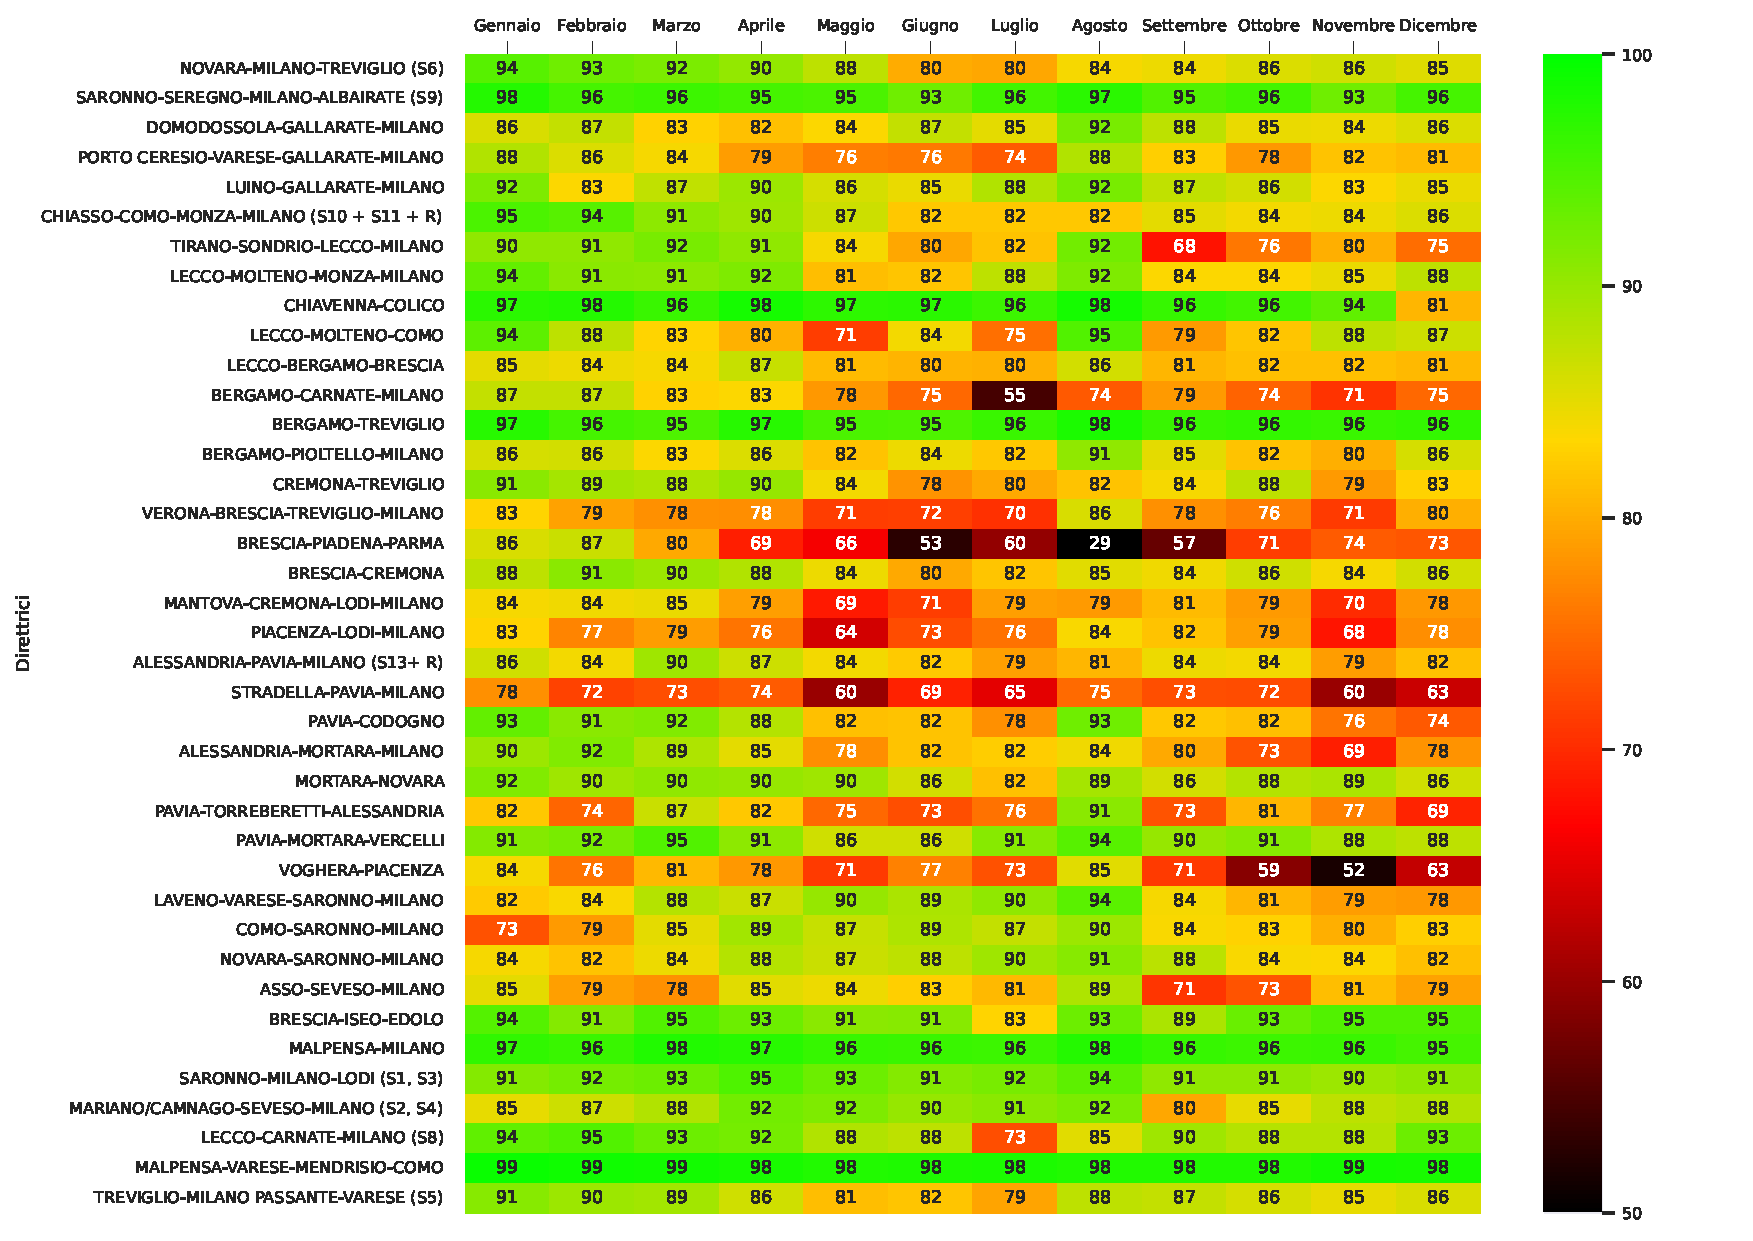
\includegraphics[width=1\textwidth]{images/lomb_heatmap.pdf}
    \caption{Indice di puntualità delle direttrici Trenord per il
        2022}
    \label{figure:lomb_heatmap}
\end{sidewaysfigure}

In \figurename~\ref{figure:lomb_heatmap}\todo{Marco: collegare foglio
    Jupyter} sono mostrati i dati trasmessi da Regione Lombardia
riguardo la \textbf{puntualità}\footnote{Come già detto, per
    \textit{indice di puntualità} si intende la percentuale di treni
    arrivata a destino con un ritardo di al più 5 minuti, escludendo
    le perturbazioni dovute a \textit{cause di forza maggiore},
    scioperi e lavori programmati} delle corse Trenord nel 2022.  La
tabella originale è stata rielaborata in modalità \textit{heatmap} per
agevolarne la lettura.  La \figurename~\ref{figure:lomb_boxplot} rende
ancora più evidente l'\textbf{importanza dei dati disaggregati}: i
dati ufficiali pubblicati sul sito della Regione (vedi
\figurename~\ref{lombardia_puntualita} e~\ref{lombardia_affidabilita})
non riescono ad esprimere accuratamente le \textbf{diverse criticità},
%\todo{AT: dire quali o referenziare sezione relativa},
che differiscono non solo per periodo ma anche per
\textbf{direttrice}.  Ad esempio, la \textit{Brescia-Paderna-Parma} ha
un indice di puntualità medio del 67.04\%, mentre la
\textit{Malpensa-Varese-Mendrisio-Como} (S40) del 98.26\%.  La
\textbf{deviazione standard} tra gli indici di puntualità medi è di
7.07.

\begin{sidewaysfigure}[p]
    \centering
    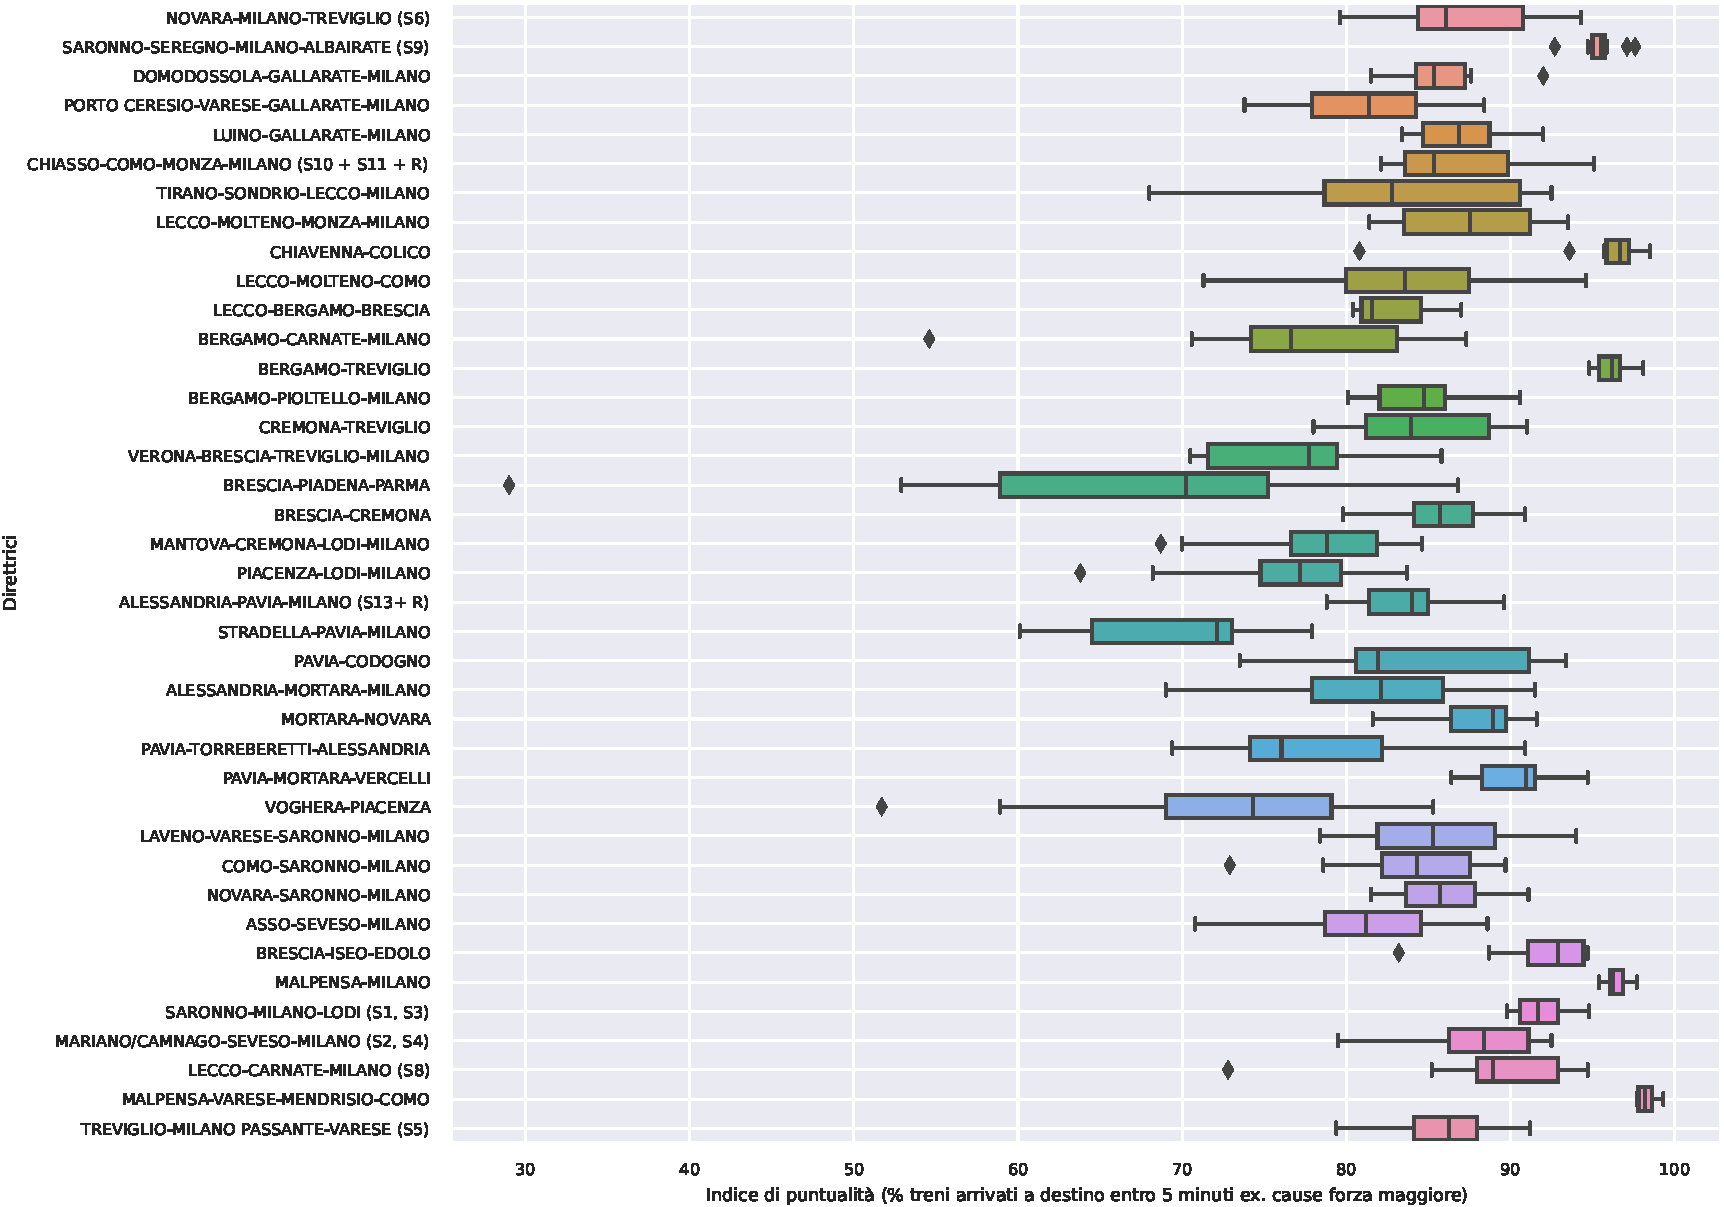
\includegraphics[width=1\textwidth]{images/lomb_boxplot.pdf}
    \caption{Boxplot dell'indice mensile di puntualità delle
        direttrici Trenord per il 2022}
    \label{figure:lomb_boxplot}
\end{sidewaysfigure}

\chapter{Progettazione e implementazione}
\label{progettazione}

In questo capitolo dell'elaborato è descritta la \textbf{parte
    implementativa} del lavoro di Tesi.  L'obiettivo è stato creare un
\textbf{software} per \textbf{scaricare} programmaticamente i dati
della circolazione ferroviaria, \textbf{renderli fruibili in formati
    aperti}
% \todo{AT: tecnicamente non è che li ``converti in opendata'' (anche
% perché non li stai rilasciando), casomai li ``rendi fruibili per una
% futura liberazione'', o simili}
e \textbf{analizzarli} proponendo statistiche descrittive e
visualizzazioni.


\section{Architettura del software}
\begin{figure}[h] \centering
    \begin{tikzpicture}[ round/.style={circle, draw=gray, minimum
            size=10mm}, rect/.style={tape, draw=gray, minimum
            size=7mm, minimum height=10mm}, bigrect/.style={rectangle,
            draw=black, minimum width=4.4cm, minimum height=15mm,
            inner sep=2.5mm, fill=cyan!50}, ]

        \node[bigrect] (scraper) at (0,0) {\textbf{\textit{Scraper}}};

        \node[rect] (viaggiatreno) [above right=12.5mm and 10cm of
        scraper.west] {API Viaggiatreno e Trenord};

        \node[bigrect] (extractor) [below=20mm of scraper]
        {\textbf{\textit{Extractor}}};

        \node[rect] (pickle) [above right=17.5mm and 10cm of
        extractor.west, anchor=west] {File \texttt{.pickle}
            incrementali};

        n \node[bigrect] (analyzer) [below=20mm of extractor]
        {\textbf{\textit{Analyzer}}}; \node[rect] (csv) [above
        right=17.5mm and 10cm of analyzer.west, anchor=west] {Dataset
            \texttt{.csv} giornalieri};
    
        \node[rect] (results) [below right=12.5mm and 10cm of
        analyzer.west] {Statistiche, visualizzazioni, \dots};

        \draw[red, <-, thick] (scraper.150) to [bend left=90,
        looseness=1] node[red, sloped, midway, fill=white] {Ogni ora}
        (scraper.30);

        \draw[gray, <-, thick] (scraper.5) -- (viaggiatreno.west)
        node[black, midway, fill=white] {scarica};

        \draw[gray, ->, thick] (scraper.355) -- (pickle.177.5)
        node[black, midway, fill=white] {salva};

        \draw[red, <-, thick] (extractor.150) to [bend left=90,
        looseness=1] node[red, sloped, midway, fill=white] {Ogni
            giorno} (extractor.30);

        \draw[gray, <-, thick] (extractor.5) -- (pickle.182.5)
        node[black, midway, fill=white] {interpreta};

        \draw[gray, ->, thick] (extractor.355) -- (csv.177.5)
        node[black, midway, fill=white] {produce};

        \draw[gray, <-, thick] (analyzer.5) -- (csv.182.5) node[black,
        midway, fill=white] {legge};

        \draw[gray, ->, thick] (analyzer.355) -- (results.west)
        node[black, midway, fill=white] {genera};
    \end{tikzpicture}
    \caption{Schema architetturale dei moduli software}
    \label{figure:architettura}
\end{figure}

Da come si evince in \figurename~\ref{figure:architettura}, il
software è composto da tre componenti.
\begin{itemize}
    \item \textbf{\textit{Scraper}}: script automatico che
    incrementalmente scarica e preserva lo stato corrente della
    circolazione ferroviaria.  Eseguito ogni ora.
    \item \textbf{\textit{Extractor}}: converte i dati dello scraper
    in file \texttt{.csv} analizzabili.  Eseguito ogni giorno.
    \item \textbf{\textit{Analyzer}}: legge i dati dai file
    \texttt{.csv} e calcola alcune statistiche e visualizzazioni
    predefinite e riproducibili.
\end{itemize}

La \textbf{modularizzazione} permette di sostituire facilmente
l'\textit{extractor} e l'\textit{analyzer} in modo da supportare più
formati e analisi.  Si ricordi infatti che lo scopo principale del
progetto non è calcolare statistiche o generare visualizzazioni, ma
fornire gli strumenti per permettere a chiunque di farlo:
\textit{bring your own format \& analyzer}.

L'unica \textbf{interfaccia utente} supportata è
CLI\footnote{\textit{Command Line Interface}, interfaccia a riga di
    comando}.  La totalità del codice è scritta in Python $\geq 3.11$
ed è rilasciata con licenza libera GPL $\geq 2.0$.

\section{Scraper}
\label{scraper}

Lo scraper è il componente più importante e complesso del sistema.  Il
suo compito è interfacciarsi con le API di Viaggiatreno e Trenord per
cercare di \textbf{reperire più informazioni possibili} sulla
circolazione ferroviaria verificando nel contempo la correttezza di
quanto letto.  Considerando che la circolazione ferroviaria è
\textit{sempre in movimento} e le API non offrono tipicamente
l'accesso ai dati storici, è inoltre fondamentale salvare le
informazioni \textbf{incrementalmente} campionando con una frequenza
opportuna.
% \todo{AT: i.e., campionando con una frequenza ``opportuna''}.
Le particolarità e i casi eccezionali, molto frequenti nelle API
considerate, devono essere gestiti \textit{incronciando} i dati con
quelli già raccolti ed eseguendo continui \textit{sanity check}.
% \todo{AT: sinonimo più esplicito, magari ``integrando/incrociando
% dati e/o calcolando informazione'')}.

\subsection{Progettazione}

\afterpage{
    \clearpage
    \newgeometry{bottom=2cm}
    \begin{landscape}
        \begin{figure}[h]
            \label{uml_classi}
            \centering
            \begin{tikzpicture}
                \tikzumlset{font=\footnotesize}
        
                \umlclass[x=0, y=0]{Train}{
                    + number: int \\
                    + origin: Station \\
                    + departing\_date: date$^*$ \\
                    + destination: Station$^*$ \\
                    + category: str$^*$ \\
                    + client\_code: int$^*$ \\
                    + departed: bool$^*$ \\
                    + cancelled: bool$^*$ \\
                    + stops: list[TrainStop]$^*$ \\
                    + delay: int  \\
                    + last\_detection\_place: str$^*$ \\
                    + last\_detection\_time: datetime$^*$ \\
                    + crowding: float$^*$ \\
                    + crowding\_source: str$^*$ \\
                    - \_phantom: bool \\
                    - \_trenord\_phantom: bool \\
                    - \_fetched: datetime$^*$ }{ + Train(number: int,
                    origin: Station, departing\_date:
                    date) \\
                    + fetch(): Train \\
                    - fetch\_trenord(): void \\
                    - \_fix\_intraday\_datetimes(): void \\
                    + arrived(): bool }

                \umlclass[right=2cm of Train.north east, anchor=north
                west]{Station}{
                    + code: str \\
                    + region\_code: int \\
                    + name: str$^*$ \\
                    + short\_name: str$^*$ \\
                    + position: [float, float]$^*$ \\
                    - \_phantom: bool \\
                    \umlstatic{- \_cache: dict[str, Station]} }{
                    + Station(code: str, region\_code: str, \\
                    \phantom{+ Station(}name: str$^*$, short\_name:
                    str$^*$, position:
                    [float, float]$^*$) \\
                    \umlstatic{+ \_from\_raw(raw\_data: dict): Station} \\
                    \umlstatic{+ by\_code(station\_code: str): Station} \\
                    \umlstatic{- \_region\_code(station\_code: str): int} \\
                    \umlstatic{+ by\_region(region\_code: int): list[Station]} \\
                    + departures(): list[Train] \\
                    + arrivals(): list[Train] }

                \umlclass[below=15mm of Station.south east,
                anchor=north east]{TrainStop}{
                    + station: Station \\
                    + stop\_type: TrainStopType \\
                    + platform\_expected: str$^*$ \\
                    + platform\_actual: str$^*$ \\
                    + arrival: TrainStopTime$^*$ \\
                    + departure: TrainStopTime$^*$ }{
                    - TrainStop(station: Station, stop\_type: TrainStopType, \\
                    \phantom{- TrainStop(}platform\_e: str$^*$, platform\_a: str$^*$, \\
                    \phantom{- TrainStop(}arrival\_e: datetime$^*$, arrival\_a: datetime$^*$, \\
                    \phantom{- TrainStop(}departure\_e: datetime$^*$, departure\_a: datetime$^*$) \\
                    \umlstatic{+ \_from\_raw\_data(stop\_data: dict):
                        TrainStop} \\
                    \umlstatic{+
                        \_from\_trenord\_raw\_data(stop\_data: dict,
                        day: date): TrainStop$^*$} }

                \umlclass[below=8.87mm of Train.south west,
                anchor=north west]{TrainStopTime}{
                    + expected: datetime \\
                    + actual: datetime$^*$ }{ +
                    TrainStopTime(expected: datetime, actual:
                    datetime$^*$)
                    \\
                    + passed(): bool \\
                    + delay(): float$^*$ }

                \umluniassoc [] {Train} {Station}

                \umluniaggreg [] {Train} {TrainStop}

                \umlcompo [] {TrainStop} {TrainStopTime}

                \umluniassoc {TrainStop} {Station}

            \end{tikzpicture}
            \caption{Diagramma UML delle classi principali}
            \vfill
        \end{figure}
    \end{landscape}
    \restoregeometry }

I requisiti di cui sopra hanno portato alla scelta del paradigma della
\textbf{programmazione ad oggetti}.  A Pagina \pageref{uml_classi} è
presente il diagramma UML delle classi principali: \texttt{Train},
\texttt{Station}, \texttt{TrainStop} e \texttt{TrainStopTime}.
Intuitivamente, ogni classe rappresenta un concetto della ferrovia e
richiama la terminologia già definita in Appendice
(\S~\ref{terminologia}).  Durante lo \textit{scraping} non tutte le
informazioni sono immediatamente disponibili: si pensi ad esempio
all'orario di arrivo effettivo di un treno in una fermata o al binario
di partenza.  Di conseguenza, i campi indicati con $^*$ possono essere
nulli.

I metodi \texttt{departures()} e \texttt{arrivals()} di
\texttt{Station} (vedi \S~\ref{partenzeArrivi}) ritornano degli
oggetti \texttt{Train} parzialmente inizializzati.  Chiamando il
metodo \texttt{fetch()} su di essi, viene letta tra le altre la
risposta API di \texttt{andamentoTreno} (vedi \S~\ref{andamentoTreno})
e sono quindi istanziati gli attributi e oggetti relativi a fermate,
stazioni e tempi tramite metodi come \texttt{\_from\_raw\_data()}.
L'\textbf{approccio \textit{top-down}} nell'inizializzazione permette
di minimizzare il numero di richieste API e delegare opportunamente le
responsabilità di decodifica e \textit{interpretazione} delle
risposte.

Le classi \texttt{ViaggiaTrenoAPI} e \texttt{TrenordAPI} espongono dei
metodi utili a interfacciarsi alle API e persistono le sessioni
HTTP/1.1+.  Le librerie \texttt{requests} e \texttt{urllib3}
permettono infatti di stabilire una connessione TCP persistente tra le
richieste e utilizzare l'algoritmo \textit{exponential backoff} in
caso di errori temporanei.

Il frequente \textit{testing} delle interfacce alle API è stato
fondamentale per correggere regressioni e cercare di coprire tutti i
casi particolari.  È stato utilizzato il framework \texttt{pytest}.

\subsection{Problemi riscontrati nelle API}

Considerare e descrivere esaustivamente tutti i casi particolari e gli
errori delle API utilizzate è quanto meno impraticabile, a causa della
mancanza di documentazione ufficiale.  Si noti inoltre che molte delle
incongruenze che saranno citate possono essere osservate anche con un
uso normale del portale Viaggiatreno.  Durante la progettazione e la
scrittura del codice sono state fatte numerose assunzioni, descritte
in seguito.

\subsubsection{Stazioni}

Osservando le risposte API del metodo \texttt{cercaStazione} di
Viaggiatreno (vedi \S~\ref{cercaStazione}) si può supporre che
\textit{tutte e sole} le stazioni italiane abbiano un \textbf{codice
    identificativo univoco} e almeno un \textbf{nome}, lungo o breve.
Ciò si verifica quasi sempre, ma si possono trovare:
\begin{itemize}
    \item \textbf{stazioni doppie}, o triple: per esempio, la stazione
    di Brescia in situazioni diverse può assumere tre codici
    differenti (\texttt{S01717}, \texttt{N00201} e \texttt{S09999});
    \item \textbf{stazioni inesistenti}: le API ritornano spesso
    stazioni che non esistono o non fanno servizio viaggiatori, come
    ``Posto Movimento Ripalta'' (\texttt{S11022});
    \item \textbf{stazioni senza nome}: 451 stazioni (il 14\%) non
    hanno nome o coordinate.
\end{itemize}

Alcune stazioni non si possono trovare tramite \texttt{cercaStazione}
(e con l'interfaccia web di Viaggiatreno) ma sono comunque presenti
nella lista delle fermate dei treni che sostano.  Un esempio è Arcene
(\texttt{S01608}), introvabile tramite la ricerca ma solo dalla lista
delle fermate di un treno sulla tratta Treviglio $\leftrightarrow$
Bergamo.  Infine, il metodo \texttt{elencoStazioni} (che dovrebbe
mostrare tutte le stazioni di una regione, vedi
\S~\ref{elencoStazioni}) può \textit{piazzare} una stazione in più
regioni differenti, anche se ciò non ha naturalmente riscontro con la
realtà.

Per facilitare le successive analisi, le stazioni con \textit{forti
    problematiche} (come la mancanza di un nome) hanno l'attributo
\texttt{\_phantom} asserito.

\subsubsection{Treni}

Durante il funzionamento normale del programma, i treni sono prima
recuperati dalle \textit{partenze} di una stazione e solo
successivamente viene interrogato il metodo \texttt{andamentoTreno}
(vedi \S~\ref{andamentoTreno}).  Talvolta, specialmente in caso di
treni parzialmente o totalmente cancellati, l'API ritorna codici di
errore come HTTP 204 (No Content) o HTTP 404 (Not Found).  In questi
casi nessuna ulteriore informazione può essere reperita, nemmeno la
lista delle fermate programmate.

Alcuni ``treni'' ritornati dall'API di Viaggiatreno ed attribuiti a
Trenord non sono \textit{corse} realmente esistenti che effettuano
servizio viaggiatori.  Si possono \textit{disambugare} le corse
fittizie da quelle reali \textit{chiedendo} informazioni a Trenord
tramite la sua API\@.  Se per Trenord la corsa non esiste allora la si
deve escludere dalle analisi.  I dati ritornati dalla API di
Viaggiatreno vengono quindi integrati con quelli dell'API di Trenord,
prediligendo la seconda in caso di conflitti.

Come già detto (vedi \S~\ref{terminologia}), un treno è identificato
univocamente anche dalla \textit{data di partenza}, in quanto
quest'ultima può essere di complicata determinazione se la corsa si
sviluppa in più giornate.  Trenord rappresenta gli orari con stringhe
\texttt{HH:MM:SS} senza le informazioni sulla data; è quindi difficile
convertirle programmaticamente in \textit{timestamp}.  Il metodo
\texttt{\_fix\_intraday\_datetimes()} di \texttt{Train} tenta di
risolvere il problema con un algoritmo che considera come appartenenti
al giorno successivo le fermate cui ora di arrivo o partenza è minore
di una costante \texttt{INTRADAY\_\-SPLIT\_\-HOUR}\footnote{La
    costante è \textit{empiricamente} impostata a 4, in quanto non ci
    sono treni operati da Trenord aventi ora di partenza prima della
    mezzanotte e ora di arrivo oltre le 4}.  Se nella prima fermata il
treno parte prima della mezzanotte, gli orari delle fermate successive
oltre la mezzanotte ed entro la soglia impostata sono aggiustati di un
giorno.

Similmente alle stazioni, i treni con dati incongruenti o che non
effettuano servizio viaggiatori hanno l'attributo \texttt{\_phantom}
asserito.

\subsection{\textit{Caching}}

Per aumentare le performance e ridurre al minimo il numero di
richieste inoltrate alle API, è stato implementato un meccanismo di
\textit{caching} delle \textbf{stazioni}.  Si suppone infatti che le
informazioni di una stazione non cambino durante l'esecuzione del
programma.  Il dizionario (\textit{hash map}) \texttt{\_cached} di
\texttt{Station} associa ad ogni \textit{codice stazione} un'istanza
della classe.  Prima di procedere con la loro esecuzione, i metodi
statici \texttt{\_from\_raw} e \texttt{by\_code} controllano la
presenza in cache della stazione richiesta; se l'oggetto non è stato
ancora creato, viene salvato in cache prima di essere ritornato.

\subsection{Algoritmo di scraping incrementale}
\label{alg_scraping}

L'obiettivo del programma è reperire più informazioni possibili da
\textbf{tutti} i treni italiani circolanti in una giornata.
Purtroppo, non esiste un metodo API che ritorna tutte le corse
circolanti in un dato momento: è necessario reperirle in altro modo.
Per risolvere il problema, si consideri che un treno circolante dovrà
necessariamente comparire nel tabellone di almeno \textit{due}
stazioni, quella di partenza e di arrivo.  Osservando i tabelloni di
\textbf{\textit{tutte} le stazioni} si possono visualizzare
\textbf{\textit{almeno tutti} i treni in circolazione}\footnote{I
    tabelloni delle partenze e degli arrivi mostrano \textit{anche}
    treni non ancora in circolazione}.  Ripetendo il processo
periodicamente è garantito poter vedere \textit{almeno due volte} ogni
treno circolato.

Per evitare di verificare lo stesso treno più volte è sufficiente
salvare le corse già viste.  Si noti che una corsa non ancora arrivata
a destinazione deve essere ricontrollata successivamente per poter
salvare i dati delle fermate non ancora superate.

\subsubsection{Descrizione ad alto livello}

\begin{algorithm}
    \caption{Scraping incrementale di tutti i treni}
    \label{alg:scraper}
    \begin{algorithmic}[1]
        \Require{Insieme $R$ delle regioni italiane}
        
        \LComment{Reperisci tutte le stazioni da tutte le regioni}
        \State $S \gets \varnothing$
        \For{$r \in R$}
            \State $S_r \gets$ \Call{stations}{$r$}
            \State $S \gets S \cup S_r$
        \EndFor

        \State \phantom{i like trains}
        \State $T \gets \varnothing$\label{alg:scraper:t}
        \Comment{Insieme dei treni non ancora arrivati}
        \State $T^* \gets \varnothing$\label{alg:scraper:ts}
        \Comment{Insieme dei treni arrivati definitivamente}
        \While{\textbf{true}}\label{alg:scraper:while}
            \LComment{Controlla lo stato dei treni non ancora arrivati
                a destino}
            \For{$t \in T$}\label{alg:scraper:for1}
                \State $t \gets $ \Call{fetch}{$t$}
                \If{\Call{arrived}{$t$}}\label{alg:scraper:for1:1}
                    \State $T^* \gets T^* \cup \{t\}$\label{alg:scraper:for1:2}
                    \State $T \gets T \setminus \{t\}$\label{alg:scraper:for1:3}
                \EndIf
            \EndFor
            \State \phantom{https://youtu.be/hHkKJfcBXcw}
            \LComment{Controlla lo stato dei treni in partenza dalle
                stazioni $S$}
            \For{$s \in S$}
                \For{$t \in $ \Call{departures}{$s$}}
                    \If{$t \in T \textbf{ or } t \in T^*$}\label{alg:scraper:for2:1}
                        \State \textbf{continue}
                        \Comment{Ignora i treni già controllati}
                    \EndIf
                    
                    \State \phantom{ }
                    \State $t \gets $ \Call{fetch}{$t$}
                    \If{\Call{arrived}{$t$}}\label{alg:scraper:for2:2}
                        \State $T^* \gets T^* \cup \{t\}$
                        \Comment{Se arrivato, salva definitivamente in $T^*$}
                    \Else
                        \State $T \gets T \cup \{t\}$
                        \Comment{Altrimenti, ricontrolla più tardi}
                    \EndIf
                \EndFor
            \EndFor
            \State \phantom{ }
            \State \Call{checkpoint}{$T, \, T^*$}\label{alg:scraper:checkpoint}
            \Comment{Salva su disco i progressi}
            \State \Call{sleep}{\text{1 hour}}\label{alg:scraper:sleep}
        \EndWhile
    \end{algorithmic}
\end{algorithm}
% \todo{AT: caption e indica che formalismo stai usando, e cita il
% tutto nel testo}

Di seguito è illustrato ad alto livello il funzionamento dello
\textit{scraper} secondo le convenzioni pseudocodice di Cormen et
al.\@~\cite{Cormen} L'unico \textbf{input} richiesto è l'insieme delle
regioni italiane $R$ utilizzato nella prima fase di popolamento
dell'insieme delle stazioni $S$.  Gli \textbf{insiemi} $T$ e $T^*$
(ll.\@~\ref{alg:scraper:t} e~\ref{alg:scraper:ts}) rappresentano
rispettivamente i \textbf{treni non ancora arrivati} (da ricontrollare
successivamente) e i \textbf{treni arrivati} (non più da controllare).

Il \textit{cuore} dell'algoritmo è un ciclo infinito
(l.\@~\ref{alg:scraper:while}) all'interno del quale sono inizialmente
ricontrollate le \textbf{corse non ancora giunte a destino}
(l.\@~\ref{alg:scraper:for1}) e che quindi hanno dati mancanti (come
l'\textit{orario effettivo} di arrivo).  Quando una corsa è arrivata
(l.\@~\ref{alg:scraper:for1:1}) allora la si salva in $T^*$ e la si
rimuove da $T$ (ll.\@~\ref{alg:scraper:for1:2}
e~\ref{alg:scraper:for1:3}).  A fine giornata l'insieme $T$ dovrebbe
essere vuoto e $T^*$ contenere tutti i treni circolati e arrivati.
Similmente, i due cicli innestati successivi iterano tra tutti i treni
in partenza da tutte le stazioni cercando \textbf{corse inedite},
ovvero non presenti in $T^*$ o $T$ (l.\@~\ref{alg:scraper:for2:1}).
Quest'ultime sono aggiunte alternativamente $T^*$ o a $T$ in base al
loro stato di arrivo (l.\@~\ref{alg:scraper:for2:2}).

Al termine di ogni iterazione, i dati sono salvati su disco (per
\textbf{persistenza}) (l.\@~\ref{alg:scraper:checkpoint}) e il
\textbf{programma si ferma} per un'ora prima di proseguire con
l'esecuzione (l.\@~\ref{alg:scraper:sleep}).  Controllare
continuamente lo stato dei treni è irragionevole e porterebbe a un
numero di richieste API esoso e ingiustificato: il \textbf{periodo di
    campionamento} di un'ora è il minimo accettabile senza rischi di
perdere anche le corse più brevi\footnote{Si noti come le corse più
    brevi di un'ora saranno comunque campionate in quanto compariranno
    nei tabelloni delle partenze ben prima dell'orario di partenza}.

\subsubsection{Note implementative}

L'algoritmo descritto precedentemente necessita di alcune accortezze
per essere implementato.  Le operazioni più comuni da
\textbf{ottimizzare} sono l'inserimento, la rimozione, l'aggiornamento
e il controllo dell'appartenenza degli elementi degli insiemi $T$ e
$T^*$.  La \textbf{struttura dati} scelta è un \textbf{hashset},
implementato in Python con un \textit{dizionario chiave-valore}.  La
chiave del dizionario è l'\textit{hash} del treno mentre il valore è
l'istanza di \texttt{Train} corrispondente.  L'hash è calcolato dalla
tripla identificativa
$(\textrm{Numero}, \, \textrm{Origine}, \, \textrm{Data})$
implementando l'API \texttt{\_\_hash\_\_} nelle classi \texttt{Train}
e \texttt{Station}.  La chiave hash \textbf{rimane costante} per la
stessa istanza tra esecuzioni diverse anche al variare degli attributi
(come gli orari delle fermate).

L'\textbf{esecuzione infinita} di un programma può risultare poco
pratica.  Per ovviare al problema si può utilizzare un applicativo
come \textbf{crontab} per implementare l'esecuzione controllata del
codice ogni ora.
% \todo{AT: da qualche parte spieghi il perché della scelta del
% periodo di campionamento?}.
La continuità e la persistenza sono ottenute grazie alla
\textbf{serializzazione} e \textbf{deserializzazione} iniziale e
finale dei dizionari \texttt{station\_cache} ($S$),
\texttt{fetched\_trains} ($T^*$) e \texttt{unfetched\_trains} ($T$)
tramite la libreria \texttt{pickle}.  Ogni notte alle 04:00 gli ultimi
due file vengono \textit{ruotati} e archiviati per la fase successiva.

Il programma utilizza Sentry\footnote{https://sentry.io} per il
monitoraggio, \textit{logging} e \textit{tracing} degli
\textbf{errori} e delle \textbf{eccezioni}.  Se sussiste un qualsiasi
problema durante il \texttt{fetch} di una risorsa, l'errore viene
catturato da Sentry ma il programma non si ferma.  Nel codice sono
presenti numerose istruzioni \texttt{assert} che prevengono
incongruenze nei dati.

Ad ogni \textit{commit} git sul branch \textit{master}, una
\textit{GitHub Action} prepara e pubblica l'immagine \textbf{Docker}
del progetto.  In questo modo, \textit{chiunque} abbia Docker
installato può avviare lo scraper con solo il seguente comando.

\begin{minted}{bash}
$ docker run \
    --volume ./data:/app/data \
    ghcr.io/marcobuster/railway-opendata:latest \
    scraper
\end{minted}

\section{Extractor}
\label{extractor}

Come detto, ogni notte lo scraper produce dei file pickle serializzati
con tutte le informazioni dei treni della giornata.  L'obiettivo
dell'extractor è \textbf{ripresentare} quanto prodotto nella fase
precedente in un formato più accessibile e prono all'analisi, anche
con linguaggi diversi da Python.  Sono stati implementati due
extractor: uno per i \textbf{treni} e uno per le \textbf{stazioni}.

\subsection{Station extractor}

I dati relativi alle stazioni, salvati dallo scraper nel file
\texttt{station.pickle}, sono convertibili dal modulo extractor in un
file CSV\footnote{\textit{Comma-separated values}, valori separati da
    virgola} o GeoJSON\footnote{JSON con informazioni sulla posizione
    geografica degli elementi.  Disponibile sono per le stazioni con
    informazioni sulla posizione}.  Ogni riga del file corrisponde una
stazione.  I campi esportati sono descritti nella \tablename\
\ref{table:station_fields}.

\begin{table}[h] \small
    \begin{tabular}{m{2cm} || m{1.7cm} | m{3cm} | m{6cm}}
      \textbf{Campo} & \textbf{Tipo} & \textbf{Descrizione} & \textbf{Note} \\
      \hline \texttt{code} & Stringa & Codice stazione & Controintuitivamente,
                                                         questo campo non è
                                                         univoco. Una
                                                         stazione può avere
                                                         più codici. \\
      \hline \texttt{region} & Intero & Codice regione & Se zero,
                                                         sconosciuto.
                                                         Utilizzato nelle
                                                         chiamate API.\\
      \hline \texttt{long\_name} & Stringa & Nome lungo & \\
      \hline \texttt{short\_name} & Stringa & Nome breve & Può essere nullo.
      \\ \hline \texttt{latitude} & Virgola mobile & Latitudine & Può essere
                                                                  nullo. \\
      \hline \texttt{longitude} & Virgola mobile & Longitudine & Può essere
                                                                 nullo.
    \end{tabular}
    \caption{Campi presenti nel CSV delle stazioni}
    \label{table:station_fields}
\end{table}

\subsection{Train extractor}

Analogamente, i dati relativi ai treni salvati dallo scraper nei file
giornalieri \texttt{fetched\-.pickle} sono convertibili dal modulo
extractor in un file CSV.\ \ Ogni riga del file corrisponde a una
\textit{fermata} e non a un treno: essendo il loro numero variabile
non è possibile disporle in colonne.  I campi esportati sono descritti
nella \tablename\ \ref{table:train_fields}.

\begin{table}[p] \small
    \begin{tabular}{m{3.5cm} || m{1.7cm} | m{5.3cm} | m{3.5cm}}
      \textbf{Campo} & \textbf{Tipo} & \textbf{Descrizione} & \textbf{Note} \\
      \hline \texttt{train\_hash} & MD5 hash & Identificatore univoco del
                                               treno & \\
      \hline \texttt{number} & Intero & Numero di treno & Non è un
                                                          identificatore
                                                          univoco. \\
      \hline \texttt{day} & Data & Data di partenza & \\
      \hline \texttt{origin} & Stringa & Codice della stz.\ di
                                         partenza & \\
      \hline \texttt{category} & Stringa & Categoria & \\
      \hline \texttt{destination} & Stringa & Codice della stz.\ di
                                              destinazione & \\
      \hline \texttt{client\_code} & Numero & Impresa ferroviaria & Vedi
                                                                    \tablename
                                                                    \ \ref{codice_cliente}.
      \\ \hline \texttt{phantom} & Booleano & \textit{Vero} se le
                                              informazioni sul treno sono
                                              state reperite solo
                                              parzialmente & I treni con
                                                             questa flag
                                                             asserita
                                                             devono
                                                             essere
                                                             ignorati. \\

      \hline \texttt{trenord\_phantom} & Booleano & Come
                                                    \texttt{\_phantom},
                                                    ma riferito alle API
                                                    di Trenord
                                                            & I treni
                                                              con
                                                              questa
                                                              flag
                                                              asserita
                                                              devono
                                                              essere
                                                              ignorati. \\
      \hline \texttt{cancelled} & Booleano & \textit{Vero} se il treno 
                                             è marcato come cancellato \\
      \hline \texttt{stop\_number} & Intero & Numero progressivo della
                                              fermata (da 0) & \\
      \hline \texttt{stop\_station\_code} & Stringa & Codice della
                                                      stazione della
                                                      fermata & \\
      \hline \texttt{stop\_type} & Carattere & Tipo di fermata
                                                            & Può essere
                                                              \textit{origine}
                                                              (\texttt{P}),
                                                              \textit{intermedia}
                                                              (\texttt{F}),
                                                              \textit{destinazione}
                                                              (\texttt{A}) o
                                                              \textit{cancellata}
                                                              (\texttt{C}).
      \\
      \hline \texttt{platform} & Stringa & Binario della fermata & Può
                                                                   essere
                                                                   nullo. \\
      \hline \texttt{arrival\_expected} & ISO 8601 & Orario di arrivo
                                                     programmato & Può
                                                                   essere
                                                                   nullo. \\
      \hline \texttt{arrival\_actual} & ISO 8601 & Orario di arrivo
                                                   effettivo & Può
                                                               essere
                                                               nullo. \\
      \hline \texttt{arrival\_delay} & Intero & Ritardo di arrivo &
                                                                    Può
                                                                    essere
                                                                    nullo
      \\
      \hline \texttt{departure\_expected} & ISO 8601 & Orario di
                                                       partenza
                                                       programmato &
                                                                     Può
                                                                     essere
                                                                     nullo. \\
      \hline \texttt{departure\_actual} & ISO 8601 & Orario di
                                                     partenza
                                                     effettivo & Può
                                                                 essere
                                                                 nullo. \\
      \hline \texttt{departure\_delay} & ISO 8601 & Ritardo di
                                                    partenza & Può
                                                               essere
                                                               nullo. \\
      \hline \texttt{crowding} & Intero & Percentuale di affollamento
                                          della corsa & Solo per i
                                                        treni Trenord.
    \end{tabular}
    \caption{Campi presenti nel CSV dei treni}
    \label{table:train_fields}
\end{table}

\section{Analyzer}
\label{analyzer}

L'ultimo modulo del progetto è l'analizzatore.  Il suo scopo è esporre
un'interfaccia utilizzabile anche da un utente non esperto di analisi
dati per generare alcune \textbf{statistiche descrittive},
\textbf{grafici} e \textbf{visualizzazioni}.  Per funzionare necessita
di un file CSV delle stazioni e \textit{almeno un} file CSV dei treni,
entrambi generati con lo strumento precedente.  Con il modulo è
possibile \textbf{filtrare} per \textit{range di date},
\textit{imprese ferroviarie} e \textit{linee ferroviarie} oltre che
\textbf{raggruppare} per \textit{treno}, \textit{impresa ferroviaria}
o \textit{giorno della settimana}.  Le \textbf{statistiche}
disponibili sono \textit{describe}, \textit{delay\_boxplot},
\textit{day\_train\_count}, \textit{trajectories\_map},
\textit{detect\_lines} e \textit{timetable}.

L'alto numero di opzioni e personalizzazione favorisce la
\textbf{riproducibilità dei risultati} a parità di dati.

Per la manipolazione dei dati è stato utilizzata la libreria Python
\texttt{pandas}.\ \ \texttt{matplotlib} e \texttt{seaborn} sono invece
state utilizzate per il \textit{rendering} dei grafici.  Il modulo
supporta il caricamento di CSV multipli per i dati dei treni su più
giorni.  Al fine di aumentare le prestazioni, il caricamento dei file
è \textbf{parallelizzato} su processi multipli.

\subsection{Linee ferroviarie}
\label{linee_ferroviarie}

Un'analisi interessante sarebbe riuscire a qualificare affermazioni
come \textit{``i treni sulla mia linea sono spesso in ritardo''} in
\textit{query} sui dati raccolti.  È quindi necessario
\textbf{definire precisamente} il concetto di \textit{linea}.
wikiRAIL definisce una \textit{linea ferroviaria} come
\textcquote{WRLinea}{l'infrastruttura necessaria e idonea a far
    viaggiare un treno o altro convoglio ferroviario tra due località
    di servizio in un determinato momento o periodo di tempo}.  La
definizione non è molto interessante in quanto è riferita
all'\textit{infrastruttura} e non al servizio commerciale.  Nemmeno
quella di \textit{direttrice} aiuta: \textcquote{WRDirettrice}{linea
    ferroviaria avente particolari caratteristiche di importanza per
    il volume dei traffici e le relazioni di trasporto che su di essa
    si svolgono, congiungendo fra loro centri o Nodi (V.) principali
    della Rete}.  Come si possono individuare tali \textit{linee
    aventi particolari caratteristiche di importanza}?  Anche se può
risultare semplice nominare alcune direttrici (Milano
$\leftrightarrow$ Roma, Bergamo $\leftrightarrow$ Brescia), è
difficile elencarle tutte senza \textbf{analizzare tutti i contratti
    di servizio} tra gli Enti e le imprese ferroviarie.

Per proseguire con le analisi è quindi necessario \textbf{ridefinire
    il concetto} in modo qualitativo.  Ai soli fini del progetto, due
treni $t_1$ e $t_2$ si considerano appartenenti alla stessa
\textbf{\textit{linea ferroviaria}} se e solo se tutte le seguenti
condizioni sono verificate:
\begin{itemize}
    \item $t_1$ e $t_2$ sono della stessa \textbf{impresa
        ferroviaria};
    \item $t_1$ e $t_2$ hanno stessa \textbf{origine};
    \item $t_1$ e $t_2$ hanno stessa \textbf{destinazione};
    \item $F_1 = F_2$, con $F_1$ e $F_2$ gli insiemi delle fermate di
    $t_1$ e $t_2$.
\end{itemize}

Per motivi di \textit{performance} è possibile \textbf{rilassare}
l'ultima condizione confrontando solo il \textit{numero} delle
fermate\footnote{Con la \textit{definizione rilassata} i risultati
    potrebbero risultare imprecisi, in quanto esistono imprese
    ferroviarie che collegano due città con \textit{percorsi} (e
    quindi direttrici) differenti.  Se due percorsi diversi tra due
    stesse città effettuati dalla medesima impresa ferroviaria hanno
    lo stesso numero di fermate, potrebbe verificarsi una
    \textit{collisione}. Per questi motivi, non è stata utilizzata.}.
L'individuazione delle linee è implementata associando ad ogni treno
un attributo univoco \texttt{line} dato dalla combinazione degli
attributi citati sopra.  La \textit{statistica} speciale
\texttt{detect\-\_lines} genera una pagina HTML mostrante una
\textbf{lista di tutte le linee rilevate} con associato per ognuna
l'identificatore univoco.

\subsection{Filtraggio}

Come citato in precedenza, il modulo offre la possibilità di filtrare
i dati secondo diversi criteri, illustrati di seguito.

Il filtro per \textbf{\textit{range} di date} è implementato con gli
argomenti \texttt{--start\--date} e \texttt{--end\--date}.  Grazie
all'uso della libreria
\texttt{dateparser}\footnote{https://dateparser.readthedocs.io/en/latest/}
è possibile specificare a propria discrezione date in formato
\textit{meccanico} (come ``\textit{2023\--09\--08}'') ma anche
\textit{umano} (``\textit{ieri}'', ``\textit{un mese e un giorno
    fa}'', \dots).

Si possono filtrare i treni anche per \textbf{imprese ferroviarie}:
l'argomento \texttt{--railway\-companies} accetta una lista (separata
da virgole) di imprese ferroviarie.  Gli elementi dell'elenco
selezionabili i seguenti: \texttt{TRENITALIA\_\-AV},
\texttt{TRENITALIA\_\-REG}, \texttt{TRENITALIA\_\-IC}, \texttt{TPER},
\texttt{TRENORD}, \texttt{OBB} e \texttt{OTHER}.

L'ultimo filtro, \texttt{--railway\--lines}, è analogo al precedente e
permette di filtrare le \textbf{linee ferroviarie}.  Gli
identificativi delle linee, separati da virgola, si possono calcolare
con la già citata statistica \texttt{detect\-\_lines}.

\subsection{Raggruppamento e aggregazione}

Oltre che filtrare, il modulo permette di \textbf{raggruppare} per
treno, impresa ferroviaria e giorno della settimana ed eventualmente
\textbf{riaggregare} con le funzioni \textit{media} o \textit{ultimo}.
Per esempio, è possibile raggruppare per impresa ferroviaria le
rilevazioni di un mese e calcolare il ritardo medio.  Oppure,
raggruppando per \textit{treno} e aggregando per \textit{ultimo} si
possono avere statistiche sulle ultime fermate di ogni treno.

I parametri da linea di comando sono \texttt{--group\--by} e
\texttt{--agg\--func}.

\chapter{Analisi e risultati}
\label{analisi}
\todo{Sistema link bibliografia}

In questo capitolo verranno commentati alcuni \textbf{risultati} e
\textbf{visualizzazioni} rilevanti.  Tutti e i soli \textbf{dati
    grezzi} utilizzati sono stati raccolti dal software descritto nel
capitolo precedente: le prossime sono le \textbf{prime analisi
    indipendenti} della \textit{reale performance} della circolazione
ferroviaria italiani.  L'autore auspica che possano essere di
\textbf{ispirazione} per ulteriore ricerca più approfondita e
iniziative di \textit{citizen science} mirate al \textbf{controllo
    dell'operato} delle imprese ferroviarie e delle Pubbliche
Amministrazioni.

Grazie all'\textbf{ampia disponibilità} di dati accumulati è possibile
trarre conclusioni significative.  Ove non diversamente specificato,
le prossime analisi si intendono realizzate dai dati raccolti dallo
scraper tra il \textbf{1° aprile 2023} e il \textbf{31 agosto 2023}.

\section{Statistiche predefinite}

Il modulo \textit{analyzer} (vedi \S~\ref{analyzer}) offre alcune
\textbf{visualizzazioni predefinite} descritte in seguito.  Uno dei
requisiti progettuali del modulo è la \textbf{completa
    parametrizzazione} dei risultati: questo favorisce la
\textbf{riproducibilità} ma rende difficile prevedere analisi più
complesse e specifiche.  Ulteriori risultati saranno discussi nella
sezione successiva (\S~\ref{altre_analisi}).

\subsection{\texttt{describe}}
\label{stat_describe}

Con l'opzione \texttt{--stat describe} l'\textit{analyzer} mostra
l'output del metodo
\texttt{describe()}\footnote{\href{https://pandas.pydata.org/docs/reference/api/pandas.DataFrame.describe.html}{https://pandas.pydata.org/docs/reference/api/pandas.DataFrame.describe.html}}
del DataFrame \texttt{pandas} considerato (al netto quindi di filtri,
raggruppamenti e riaggregazioni).

% \begin{minted}[fontsize=\small]{bash}
% $ python main.py analyze \
%     --start-date '2023-04-01' \
%     --end-date '2023-08-31' \
%     --stat describe \
%     'data/stations.csv' \
%     'data/2023-0{4,5,6,7,8}-??/trains.csv'
% \end{minted}

% https://paste.studentiunimi.it/paste/6aowvjOF#Pj-GUSbCCy5D9exYMMrkRoFueW0HyKmbhTX5sKrjCD+
\begin{table}[h]
    \begin{tabular}{r|ccc}
      \textbf{Statistica} & \textbf{Rit.\@ arrivo} (min) & \textbf{Rit.\@ partenza} (min) & \textbf{Affollamento} (\%)
      \\ \hline Conteggio & $9.98 \cdot 10^6$ & $1.12 \cdot 10^7$  & $2.62 \cdot 10^6$
      \\ Media & $2.81$ & $3.99$ & $2.32$
      \\ Dev.\@ Std.\@ & $8.13$ & $7.37$ & $5.34$
      \\ 1° quartile & 0.00 & 1.00 & 10.83
      \\ 2° quartile & 1.00 & 2.00 & 19.00
      \\ 3° quartile & 3.50 & 4.50 & 31.00 
    \end{tabular}
    \caption{Statistiche descrittive dei treni italiani dal 31/03/2023
        al 31/08/2023}
    \label{table:describe}
\end{table}

Dai dati presentati in \tablename~\ref{table:describe} emergono alcuni
aspetti interessanti.  Si può inanzitutto notare che il
\textbf{ritardo in arrivo} è generalmente minore del \textbf{ritardo
    in partenza}: nel 76\% delle fermate considerate il treno riesce a
\textbf{recuperare ritardo} e nell'89\% non lo accumula ulteriormente
(vedi \figurename~\ref{figure:delay_var}).  Questo effetto è
probabilmente amplificato dal fatto che ad un treno è concesso di
\textbf{arrivare in anticipo} ma non di partire prima dell'orario
programmato.

L'\textbf{affollamento}\footnote{Si ricorda che i dati
    sull'affollamento sono disponibili solo per i treni Trenord}
rilevato è tendenzialmente basso: la probabilità che questo superi
l'80\% è solo dell'1.83\%~\cite[B]{StatJup}.  Il dato è da prendere
con adeguata \textbf{diffidenza} in quanto è fornito in conflitto di
interesse da Trenord stessa, i metodi di calcolo non sono noti e il
risultato non è facilmente verificabile.

\begin{figure}[h] \centering
    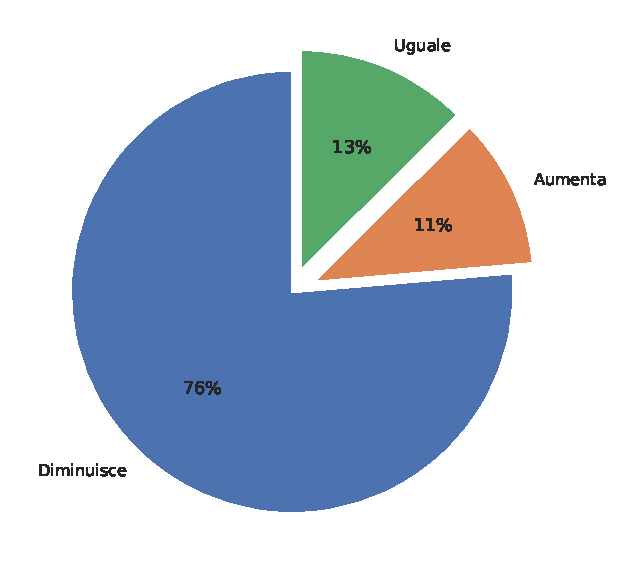
\includegraphics[width=0.5\textwidth]{images/delay_var.pdf}
    \captionof{figure}{Variazione del ritardo tra l'arrivo e la
        partenza in una fermata~\protect{\cite[A]{StatJup}}}
    \label{figure:delay_var}
\end{figure}

\subsection{\texttt{delay\_boxplot}}
\label{stat_delay_boxplot}

L'opzione \texttt{--stat delay\_\-boxplot} permette di visualizzare
un boxplot dei dati sui \textbf{ritardi} in arrivo e partenza del
campione selezionato.

Un \textit{boxplot} (o \textit{diagramma a scatola e baffi}) è un
\textbf{rappresentazione grafica} delle statistiche principali di un
campione (vedi \figurename~\ref{figure:boxplot}).  I bordi della
\textit{scatola} rappresentano il 1° e il 3° quartile, mentre i
\textit{baffi} il valore minimo e massimo.  Gli \textit{outliers} sono
valori anomali molto distanti dagli altri; considerata la loro
quantità nei dati considerati, sono stati nascosti per aumentare la
comprensione.

\begin{figure}[h] \centering
    \begin{tikzpicture}[scale=0.9]

        \draw (-1,0) rectangle (3,1); % box

        % frecce + label
        \draw[<-] (-1, -0.1) -- (-1, -0.4) node[anchor=north] {1°
            quartile}; \draw[<-] (3, -0.1) -- (3, -0.4)
        node[anchor=north] {3° quartile};

        \draw (-2.5, 0.25) -- (-2.5, 0.75) node[anchor=south]
        {minimo}; % baffo sinistro
        \draw (-1, 0.5) -- (-2.5, 0.5); % linea sinistra

        \draw[line width=0.4mm] (2.5, 0) -- (2.5, 1) ; % mediana

        \draw[<-] (2.5, 1.1) -- (2.5, 1.4) node[anchor=south]
        {mediana};

        \draw (3, 0.5) -- (6, 0.5); % linea destra
        \draw (6, 0.25) -- (6, 0.75) node[anchor=south]
        {massimo}; % baffo destro

        % outliers sinistri
        \draw (-6.5, 0.5) circle (0.5mm); \draw (-5.4, 0.5) circle
        (0.5mm); \draw [decorate,decoration={calligraphic brace}]
        (-6.6, 0.7) -- (-5.3, 0.7) node [pos=0.5,above=0.5mm]
        {\textit{outliers}};

        % outliers destri
        \draw (8.0, 0.5) circle (0.5mm); \draw (9.5, 0.5) circle
        (0.5mm); \draw [decorate,decoration={calligraphic brace}]
        (7.9, 0.7) -- (9.6, 0.7) node [pos=0.5,above=0.5mm]
        {\textit{outliers}};

    \end{tikzpicture}
    \caption{Struttura di un boxplot}
    \label{figure:boxplot}
\end{figure}

Come già detto, il modulo supporta il \textbf{raggruppamento}.  La
\figurename~\ref{figure:delay_box_rc} è il risultato dell'invocazione
del modulo raggruppando i dati per \textbf{impresa ferroviaria}.
Appare evidente che i \textbf{treni a lunga percorrenza} (alta
velocità e intercity) sono generalmente \textbf{più in ritardo} dei
regionali (Trenitalia, Trenord e Tper).  La \textbf{durata maggiore}
dei primi può spiegare il fenomeno; si può considerare \textit{meno
    rilevante} un ritardo di pochi minuti su un \textbf{viaggio lungo}
(nonostante il disagio per il viaggiatore, specialmente in caso di
coincidenze, sia potenzialmente lo stesso).

Tra le tre \textbf{imprese ferroviarie regionali} considerate è lecito
affermare che nel periodo considerato la \textbf{\textit{performance}
    peggiore} --- in termini di \textbf{ritardo mediano} --- è
attribuibile a \textbf{Trenord} (1.5 minuti in arrivo e 2.5 minuti in
partenza), quasi a parimerito con \textbf{Tper} (1.5 min e 2.0
min).\@~\textbf{Trenitalia} (1.0 min e 2.0 min) ha il ritardo mediano
più contenuto, anche se di poco~\cite[C]{StatJup}.  Analisi successive
tenteranno di confermare o sfatare queste conclusioni preliminari.

In \figurename~\ref{figure:delay_box_wd} è mostrata la stessa
visualizzazione raggruppando per \textbf{giorno della settimana}.  Dal
grafico è possibile notare un \textbf{leggero andamento crescente} con
da lunedì e venerdì e una \textbf{discesa} nel weekend, sabato e
domenica.  Le differenze tra giorni feriali e fine settimana potrebbe
essere dovuta al diverso \textbf{numero di treni circolanti}: i dati
successivamente suggeriranno \textbf{correlazione} tra ritardo e
numero di treni.  I maggiori ritardi del \textbf{venerdì} potrebbero
essere dovuti alla maggiore frequenza di \textbf{scioperi}.

\begin{figure}[p] \centering
    \subfloat[raggruppati per impresa ferroviaria]{
        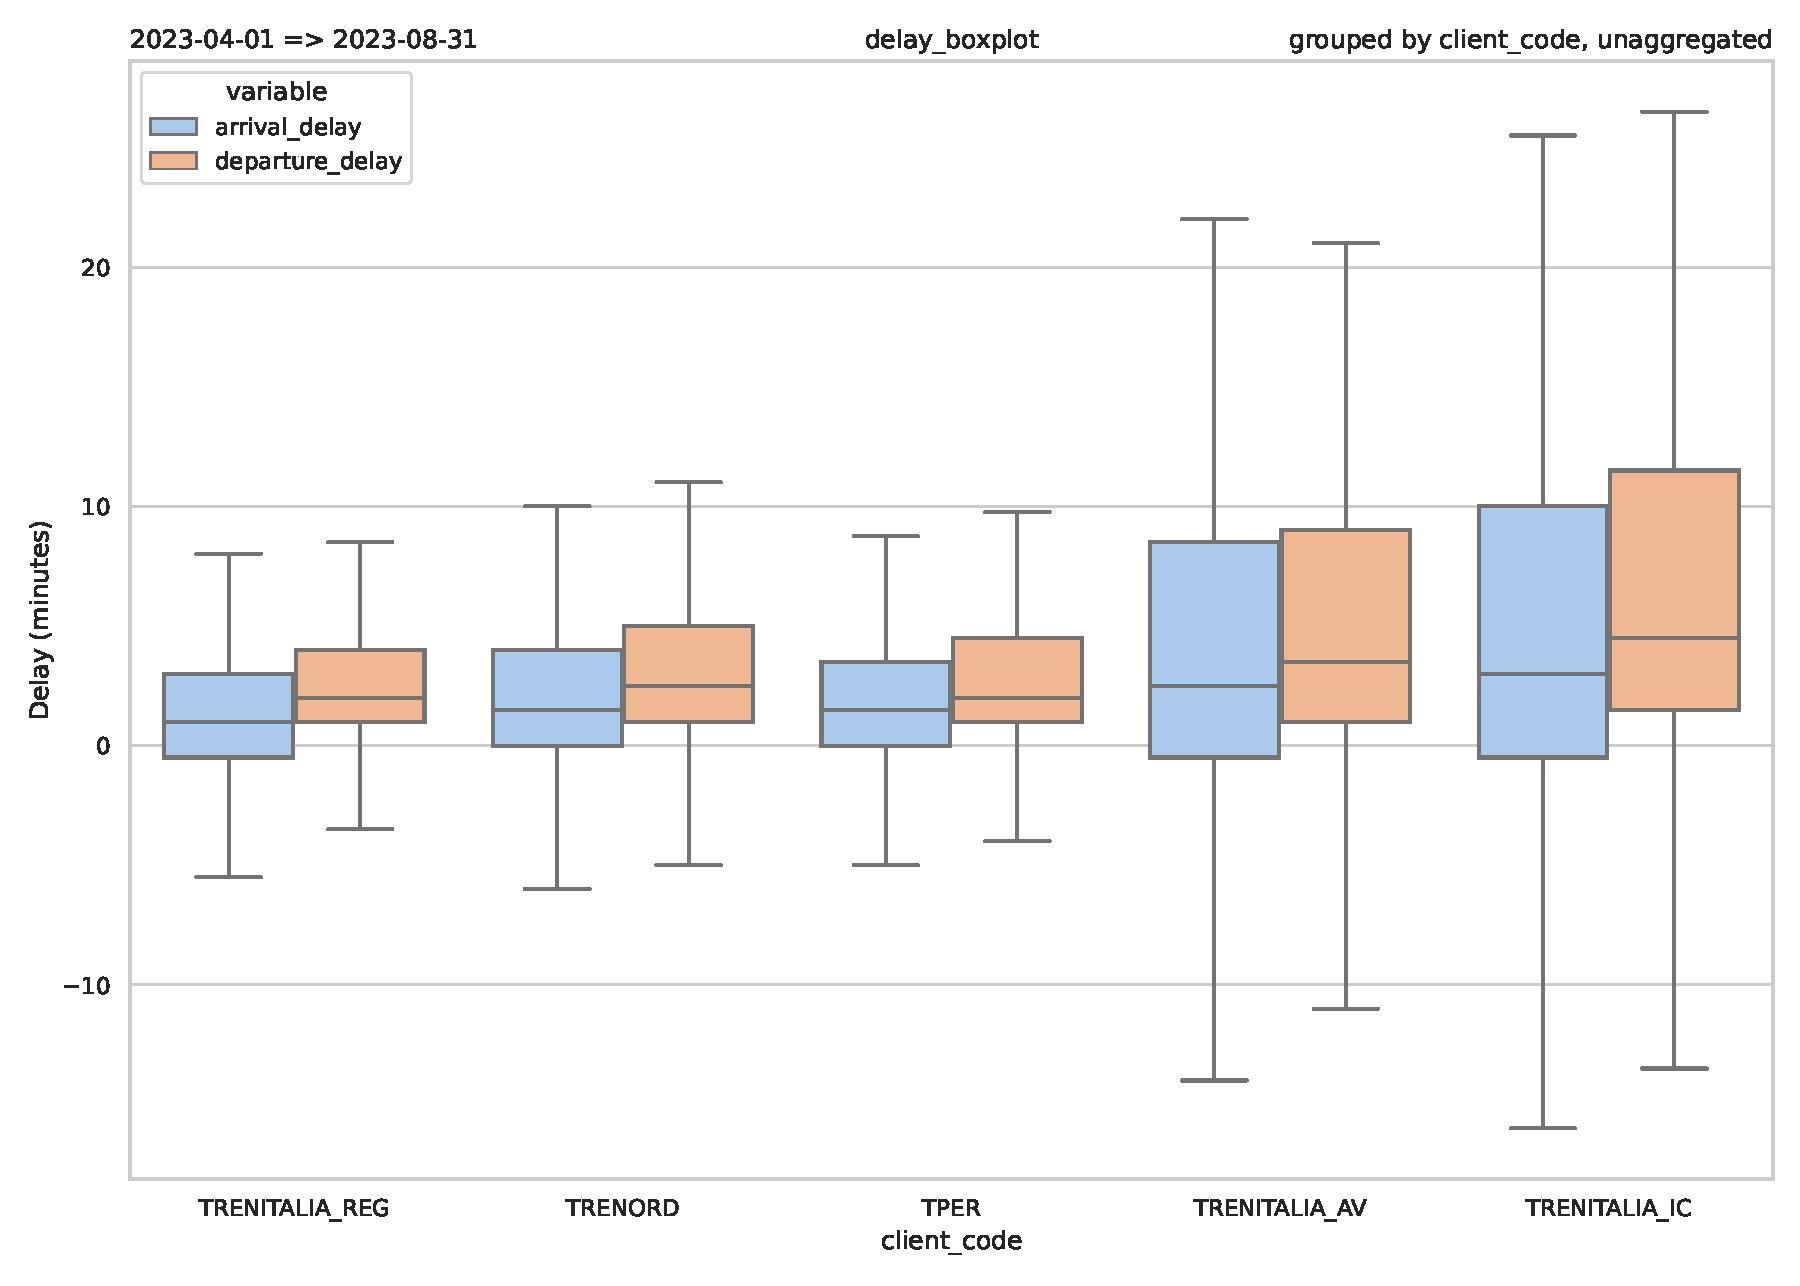
\includegraphics[width=0.95\textwidth]{images/delay_box_rc.pdf}
        \label{figure:delay_box_rc}
    } \vspace{5mm}
    \subfloat[raggruppati per giorno della settimana]{
        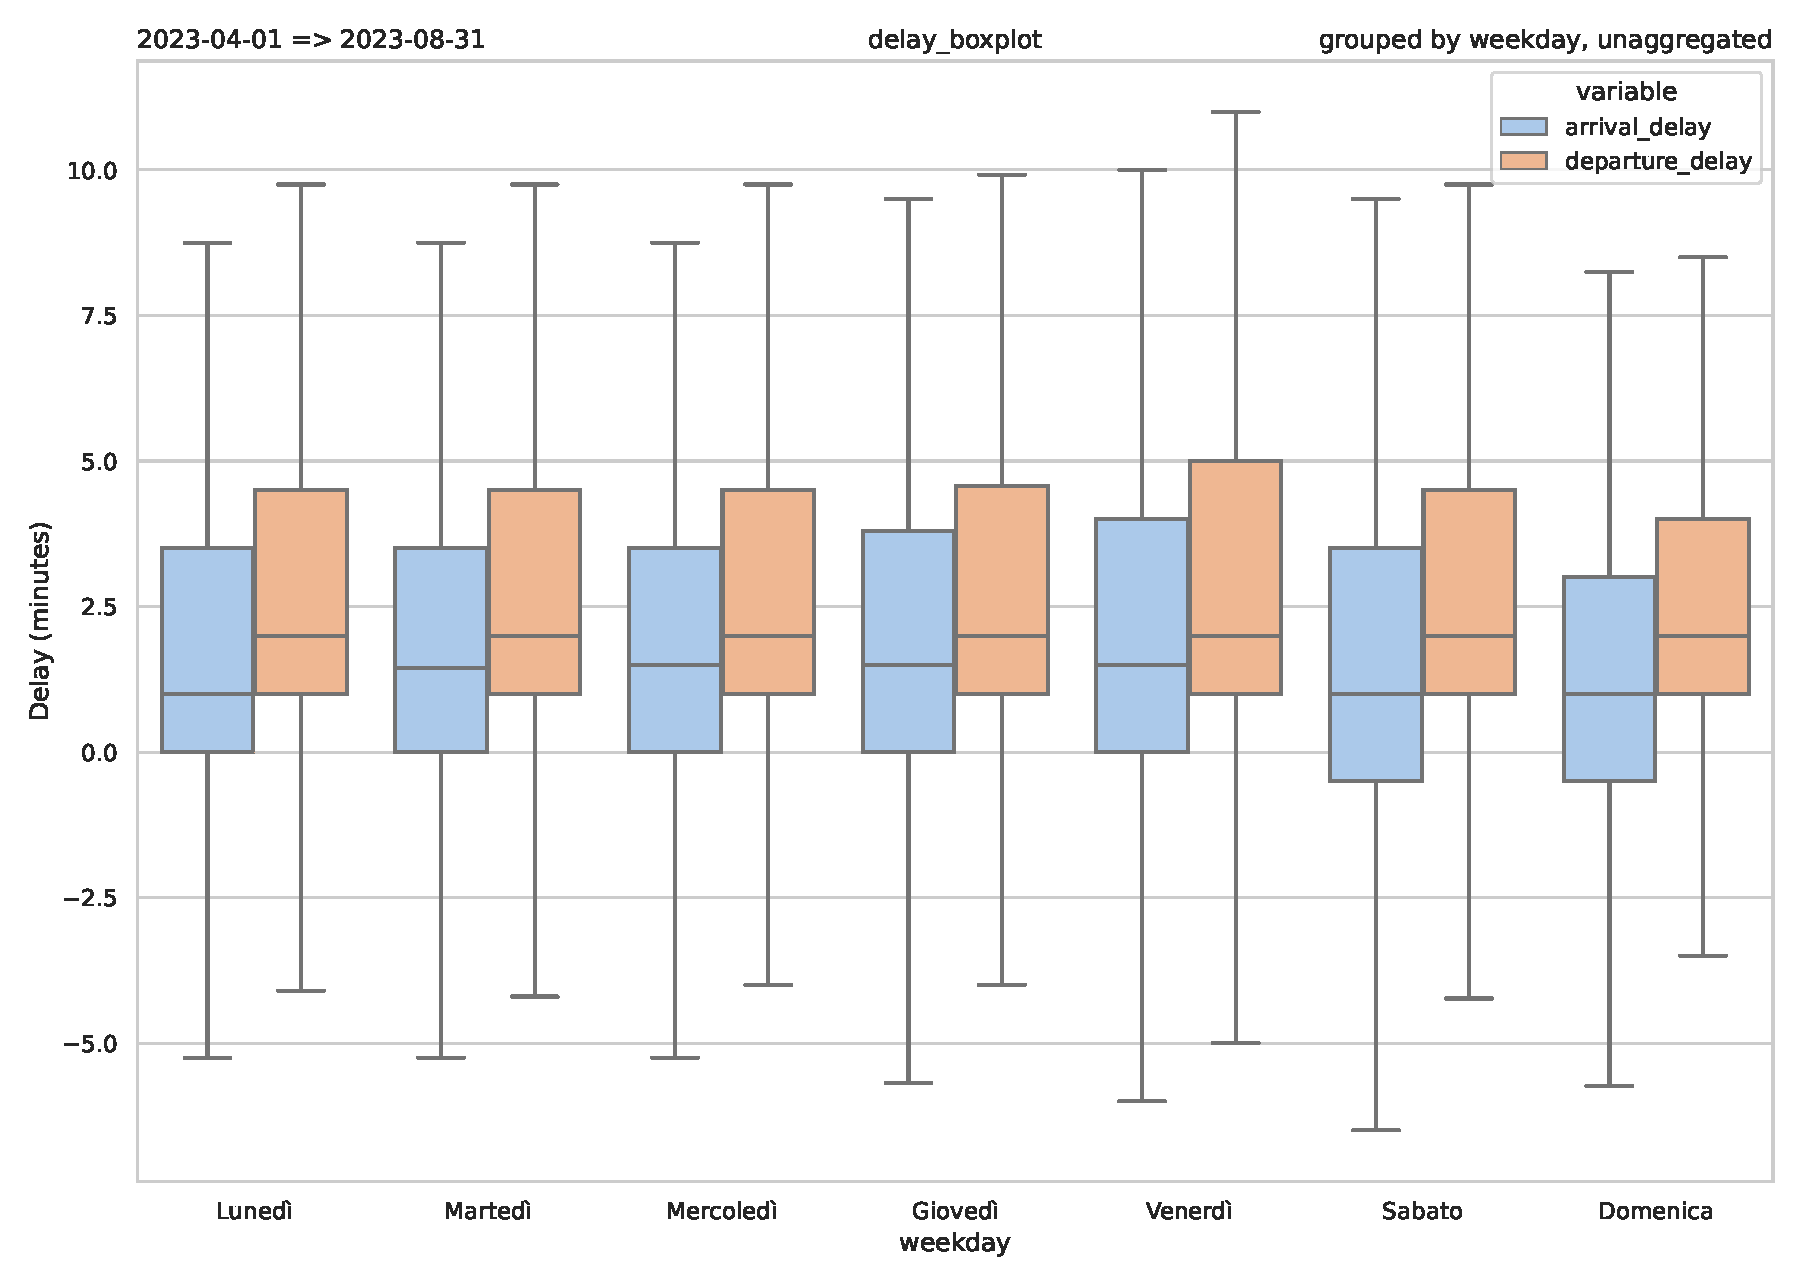
\includegraphics[width=0.95\textwidth]{images/delay_box_wd.pdf}
        \label{figure:delay_box_wd}
    }
    \caption{Boxplot dei ritardi dei treni italiani}
\end{figure}

\subsection{\texttt{day\_train\_count}}
\label{stat_day_train_count}

Un'altra statistica interessante è l'andamento del \textbf{numero di
    treni circolanti} nel corso delle giornate.  Con l'opzione
\texttt{--stat day\_\-\_train\_\-count} è possibile visualizzare il
numero di treni circolati per ogni giornata considerata.

La \figurename~\ref{figure:day_train_count} è il risultato
dell'invocazione sui dati del mese \textbf{aprile 2023} senza
ulteriori raggruppamenti.  Si osservi come il numero di treni
\textbf{varia notevolmente} tra le giornate: in media hanno viaggiato
7697 treni al giorno, con un mediana di 8833 treni e un massimo di
9141 \cite[D]{StatJup}.  La \textbf{giornata peggiore} è stata
domenica 30 aprile 2023, con soli 2773 treni circolati a causa di uno
sciopero nazionale.  Raggruppando per \textbf{impresa ferroviaria}
(vedi \figurename~\ref{figure:day_train_count_rc}) si può inoltre
osservare l'\textbf{elevato numero} di corse effettuate da Trenitalia
(regionale) e Trenord rispetto alle altre imprese ferroviarie.  La
citata diminuzione di traffico nel fine settimana è meno accentuata
per i \textbf{treni a lunga percorrenza}, i quali mantengono il
servizio anche secondo logiche di mercato.

\subsection{\texttt{detect\_lines}}

\begin{figure}[h]
    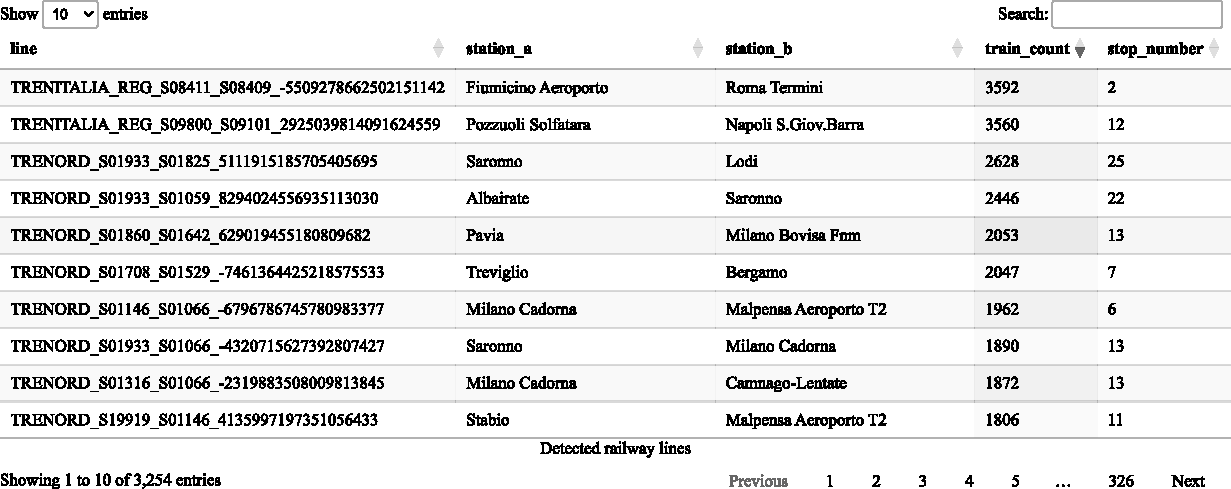
\includegraphics[width=1\textwidth]{images/detect_lines.pdf}
    \caption{Linee ferroviarie rilevate nel mese di giugno 2023}
    \label{figure:detect_lines}
\end{figure}


\begin{figure}[p] \centering
    \subfloat[raggruppati per ogni giornata nel mese di aprile 2023]{
        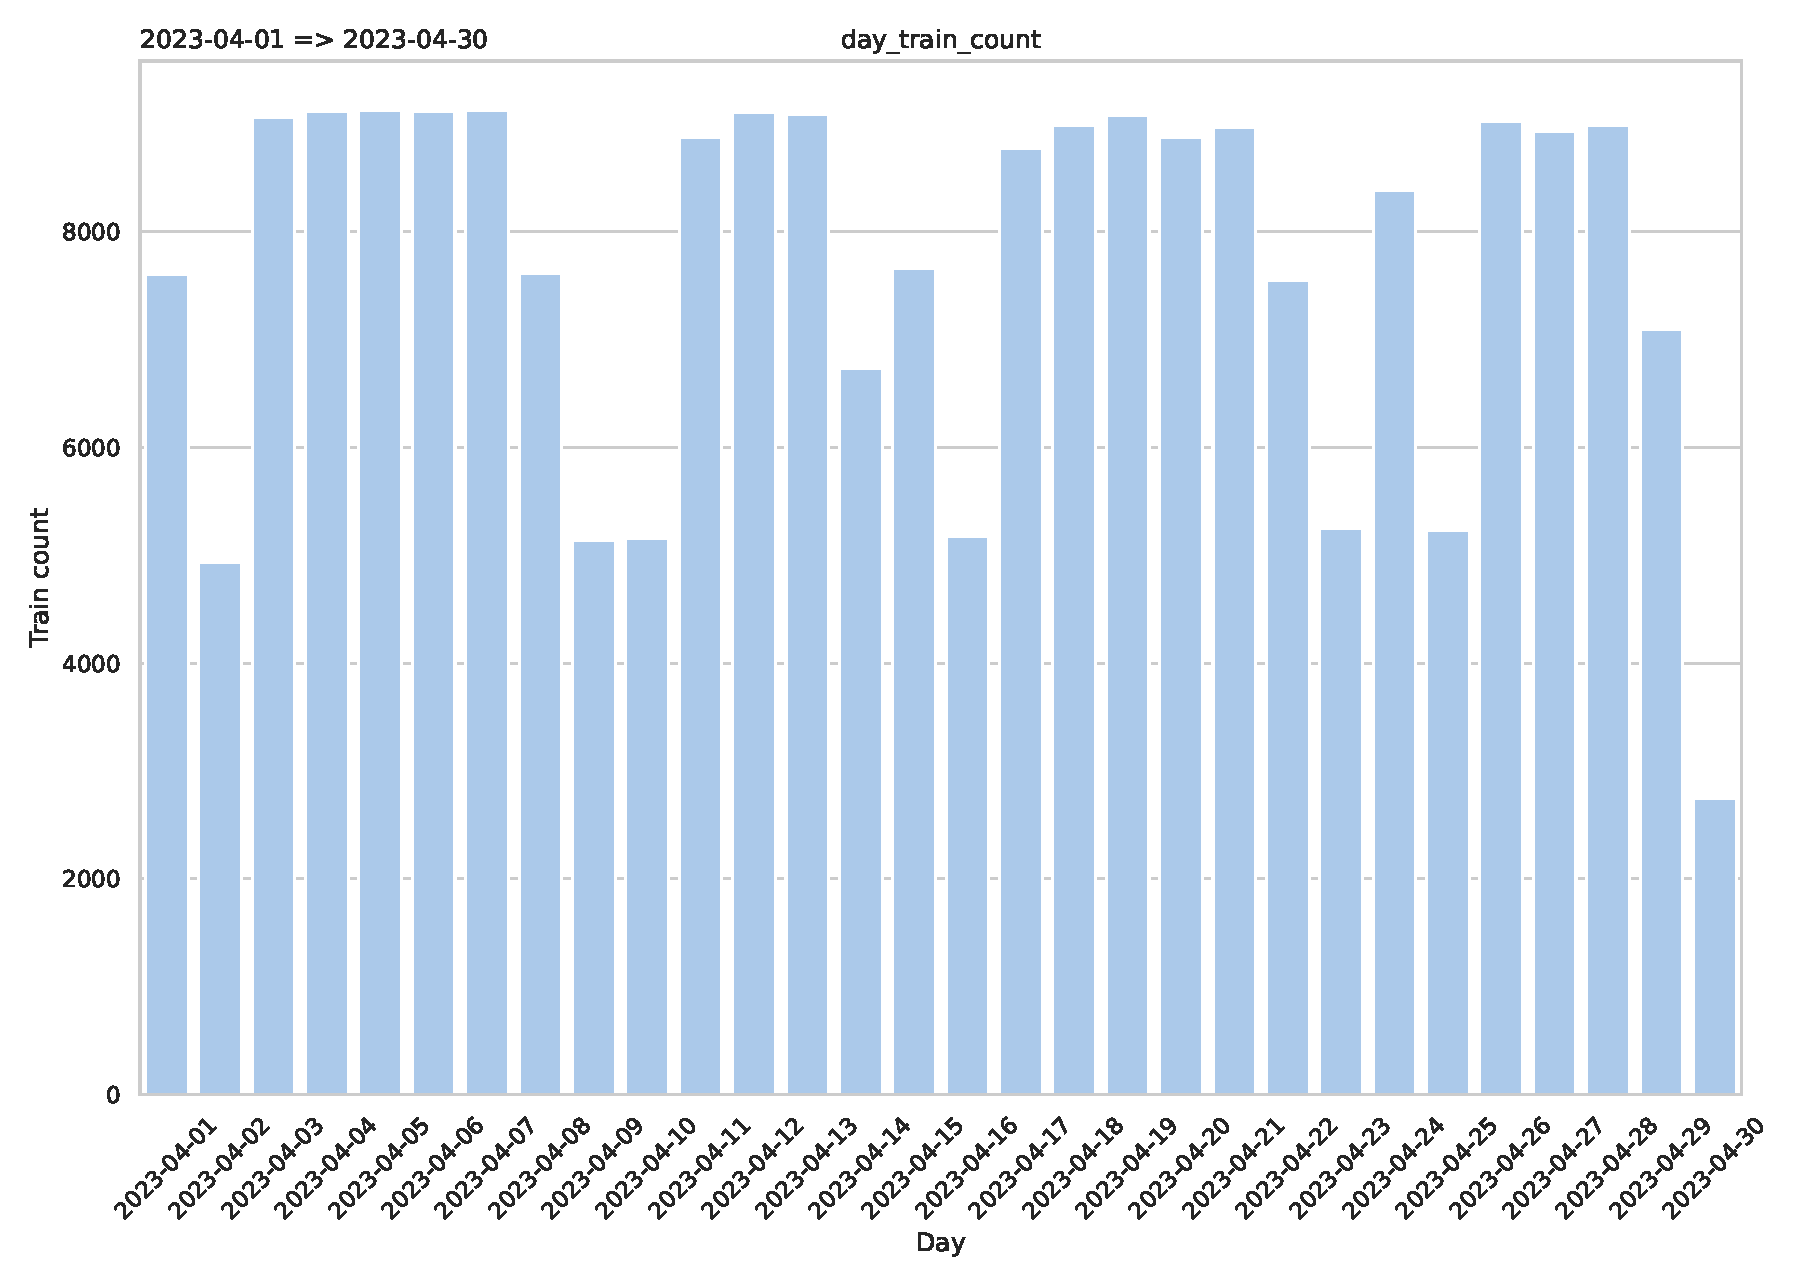
\includegraphics[width=0.95\textwidth]{images/day_train_count.pdf}
        \label{figure:day_train_count}
    } \vspace{5mm}
    \subfloat[raggruppati per impresa ferroviaria, da lunedì
    08/05/2023 a domenica 14/05/2023]{
        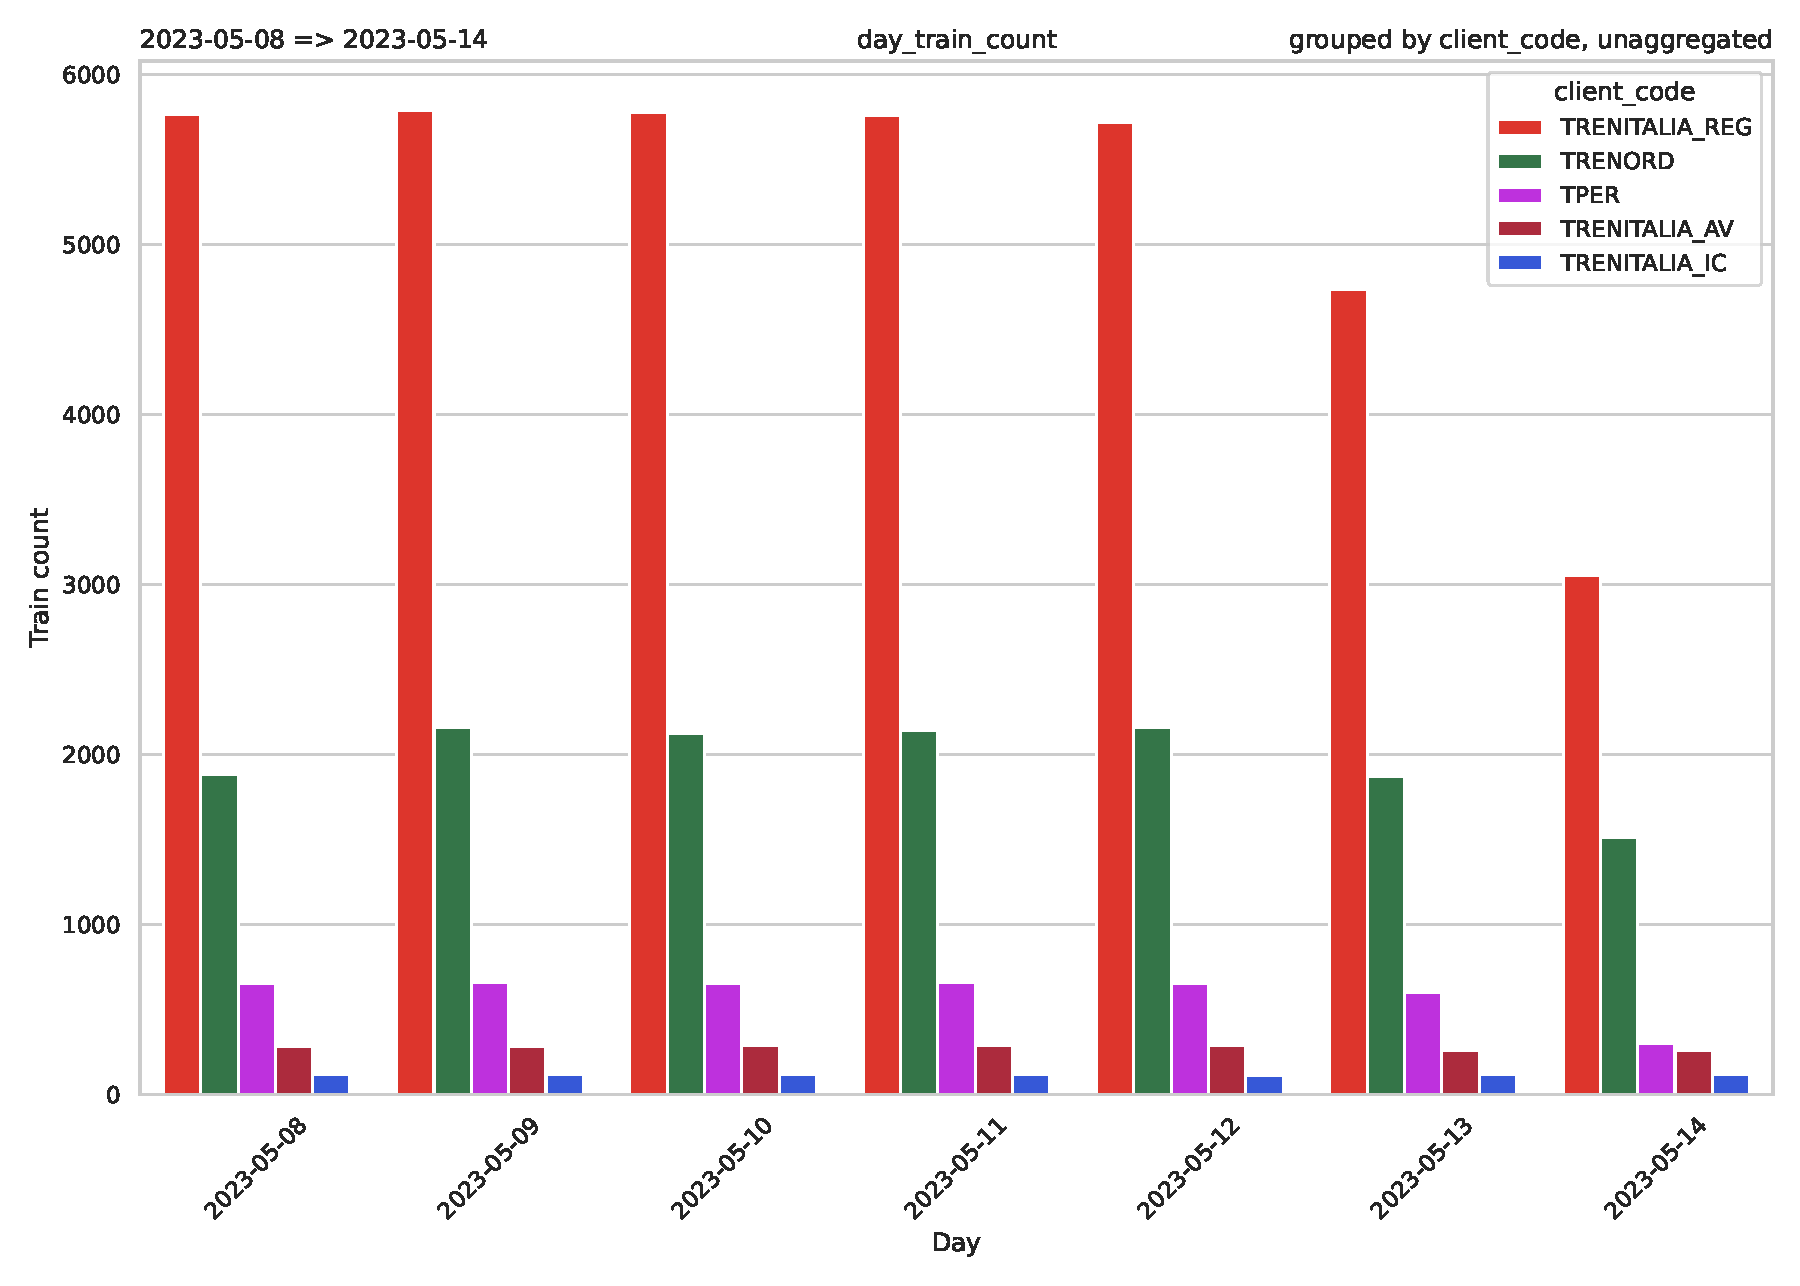
\includegraphics[width=0.95\textwidth]{images/day_train_count_rc.pdf}
        \label{figure:day_train_count_rc}
    }
    \caption{Numero di treni circolanti}
\end{figure}

Precedentemente (vedi \S~\ref{linee_ferroviarie}) è stata proposta una
definizione puntuale di \textbf{linea ferroviaria}.  Riassumendo, due
treni $t_1$ e $t_2$ appartengono alla stessa \textit{linea} se e solo
se sono operati dalla stessa impresa ferroviaria e hanno eguale
\textit{insieme delle fermate}.  L'\textit{analyzer} assegna ad ogni
linea un \textbf{identificatore univoco}, prodotto delle proprietà di
cui sopra e utilizzabile successivamente per filtrare o raggruppare i
dati.  L'opzione \texttt{--stat detect\_\-lines} genera e apre una
pagina HTML contenente una tabella di tutte le linee rilevate (vedi
\figurename~\ref{figure:detect_lines}).  Le colonne della tabella
% (\textit{identificativo linea}, \textit{stazione A},
% \textit{stazione B}, \textit{numero di treni} e \textit{numero di
% fermate})
possono essere utilizzate come \textbf{criterio di ordinamento} e
filtrate tramite la \textbf{barra di ricerca}.

\subsection{\texttt{timetable}}
\label{stat_timetable}

\begin{figure}[p] \centering
    \subfloat[visualizzazione della giornata]{
        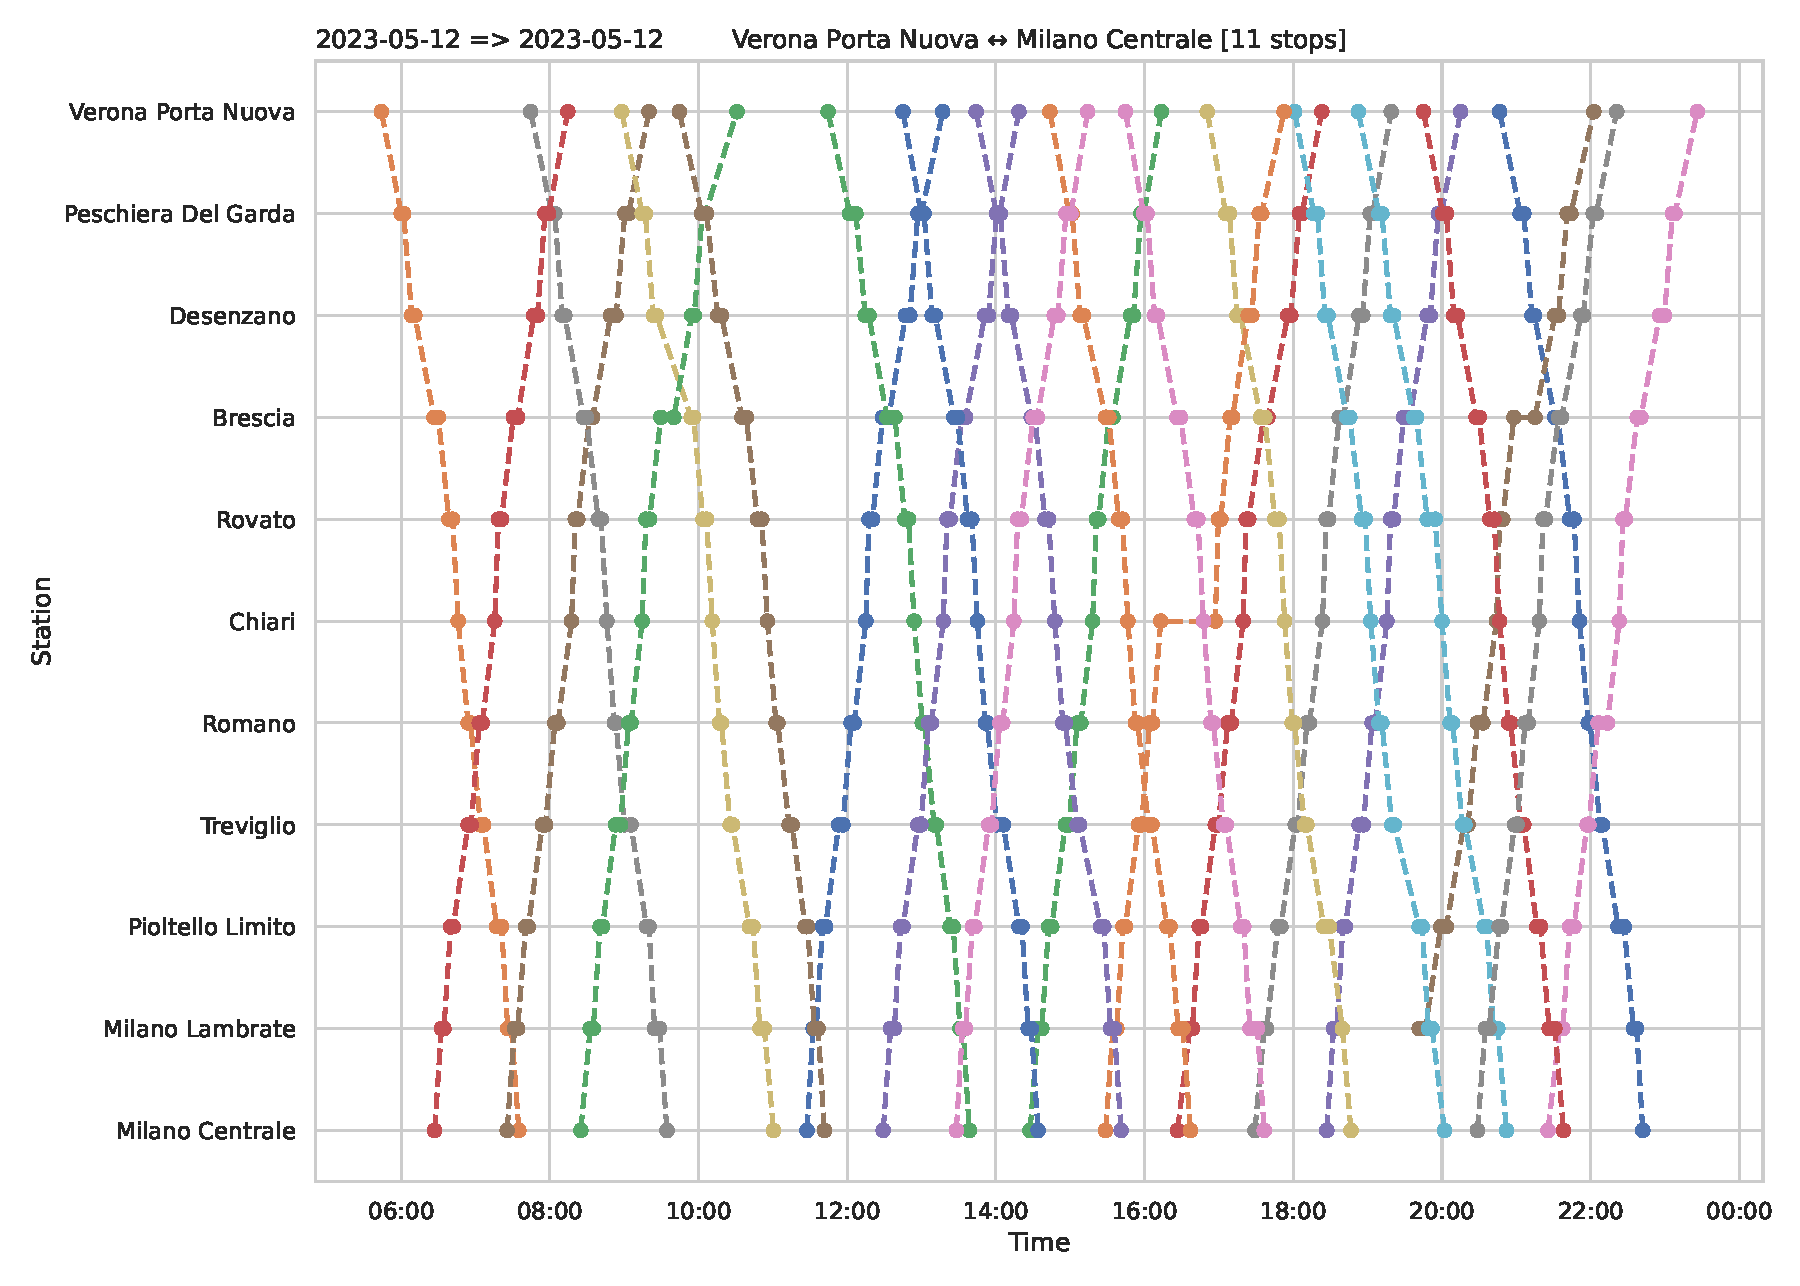
\includegraphics[width=0.95\textwidth]{images/timetable.pdf}
        \label{figure:timetable_uncollapse}
    } \vspace{5mm}
    \subfloat[visualizzazione delle durate]{
        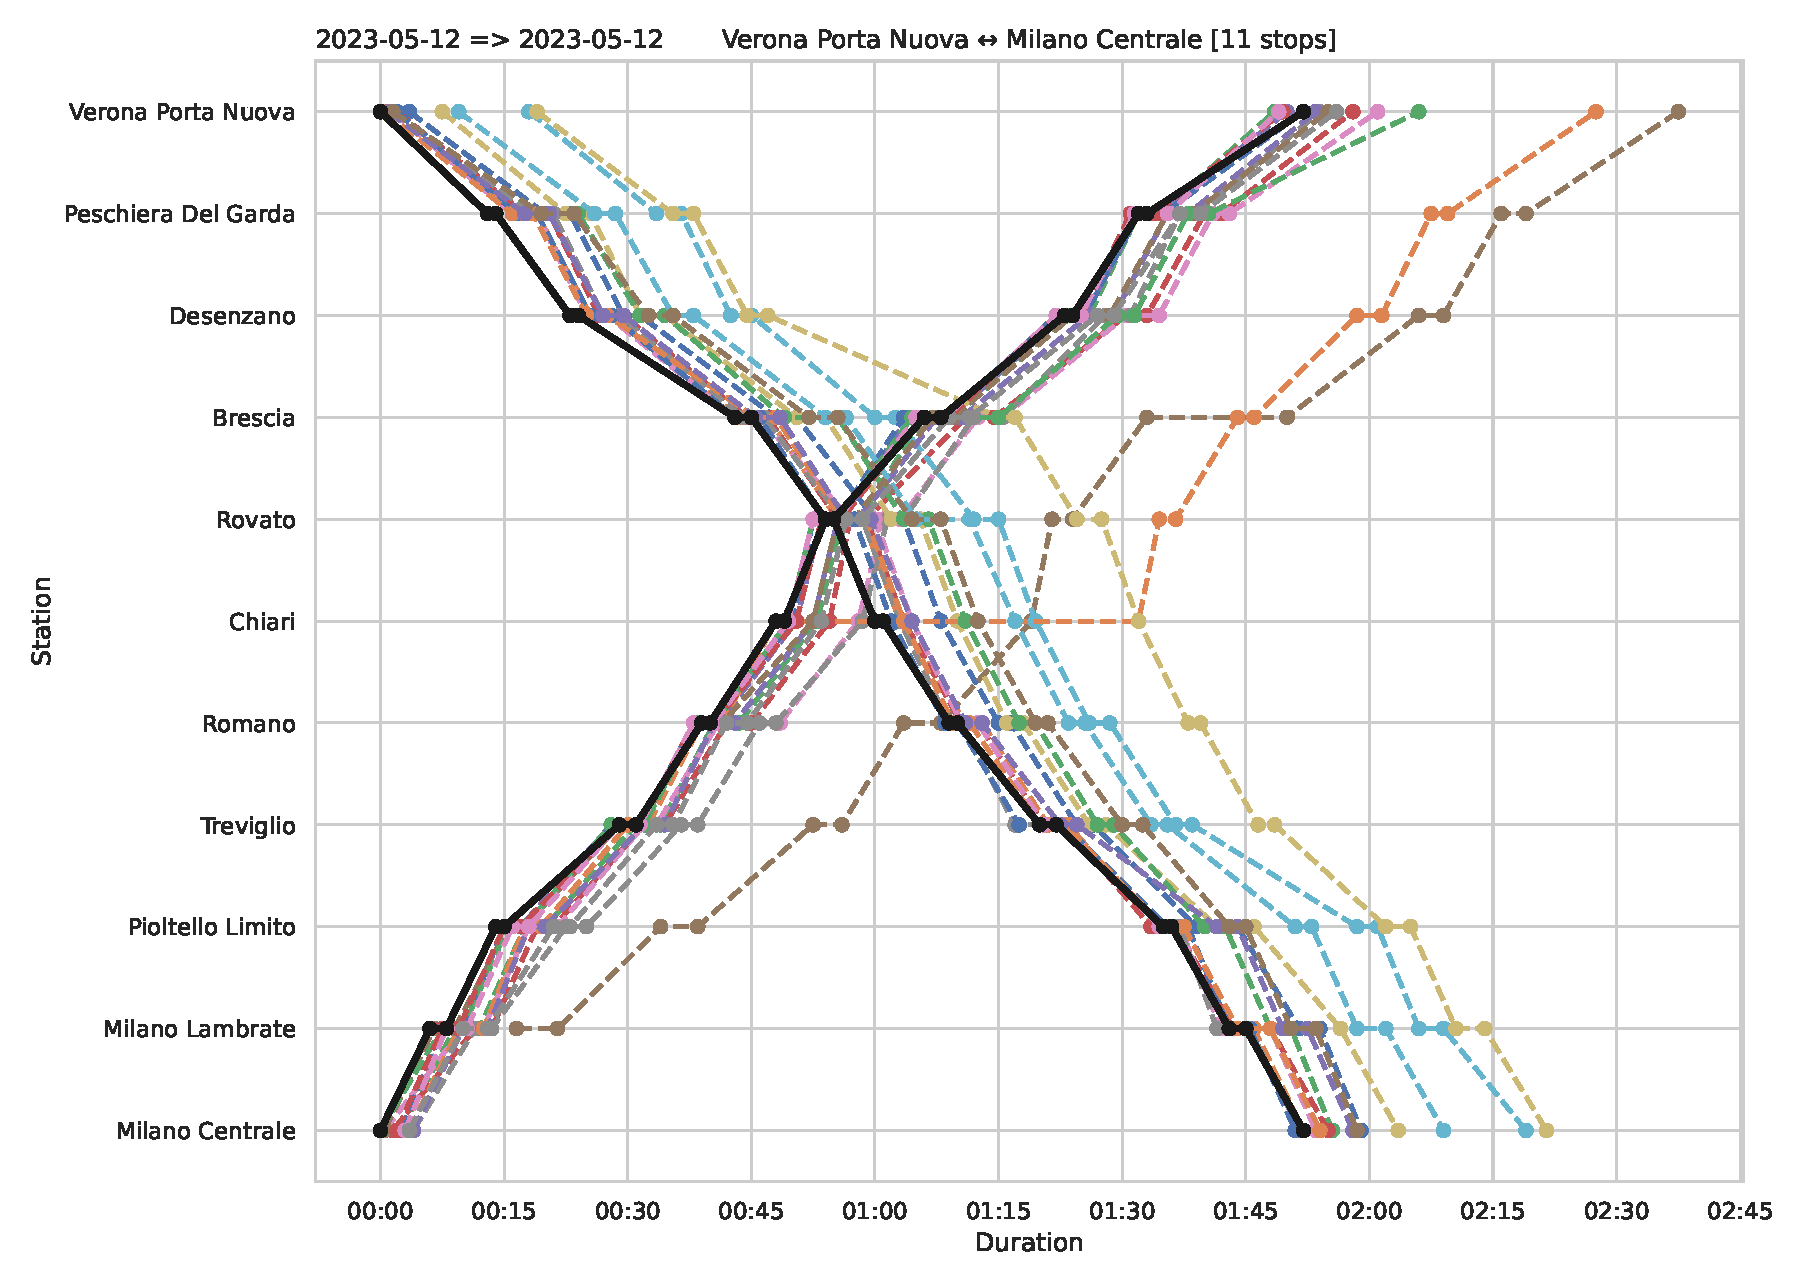
\includegraphics[width=0.95\textwidth]{images/timetable_collapse.pdf}
        \label{figure:timetable_collapse}
    }
    \caption{\textit{Orario grafico} della linea Verona Porta Nuova
        $\leftrightarrow$ Milano Centrale, del 12/05/2023}
    \label{figure:timetable}
\end{figure}

RFI mette a disposizione al proprio personale autorizzato e alle
imprese ferroviarie la c.d.\@ ``PIC'' (Piattaforma Integrata
Circolazione).  Tra gli innumerevoli servizi offerti \cite{RfiPic}
(come ASTROIF, per le comunicazioni tra IF e GI e ExtraPMdA, per i
servizi di manutenzione dei treni) è presente il c.d.\@
``\textbf{orario grafico}'', un complesso grafico avente come ascissa
il \textbf{tempo} e ordinata le \textbf{località} di una direttrice.
I \textbf{treni in circolazione} sono rappresentati da delle linee
colorate che collegano i punti sul piano; le \textbf{interruzioni di
    linea} sono graficate con rettangoli rossi.  Il
DCO\footnote{Dirigente Centrale Operativo, detto informalmente
    \textit{capostazione}} utilizza costantemente le tracce orario per
coordinare la circolazione e avere una visione d'insieme rilevante.
Essendo la piattaforma inaccessibile pubblicamente, non è possibile
allegare immagini o ulteriore documentazione alla presente
descrizione.  L'opzione \texttt{--stat timetable} cerca di
\textbf{emulare} le tracce orario RFI: selezionata una linea e i dati
di una giornata, l'applicativo \textit{traccia} su un piano i percorsi
di tutti i treni circolati.  Le \figurename~\ref{figure:timetable} è
il prodotto del programma sui dati del 12 maggio 2023 della
\textit{linea} regionale Verona Porta Nuova $\leftrightarrow$ Milano
Centrale, operata da Trenord.

Il primo grafico (\figurename~\ref{figure:timetable_uncollapse}) è
progettato sulla precedente descrizione dell'orario grafico di RFI.
L'ascissa rappresenta l'\textbf{orario} nella giornata, l'ordinata le
\textbf{località}.  Ogni linea colorata (\textit{traccia}) è una
\textbf{corsa} avente origine a Milano Centrale o a Verona P.N\@.  I
punti rappresentano l'\textbf{orario effettivo di arrivo} e
\textbf{partenza} del treno nella fermata intermedia corrispondente;
in caso di ritardo in partenza, essi non saranno sovrapposti.  Nella
visualizzazione in oggetto è possibile osservare il noto \textit{buco}
di circolazione ferroviaria tra le 10:00 e le 12:00.

Ancora più interessante è la seconda visualizzazione
(\figurename~\ref{figure:timetable_collapse}) ottenuta con l'aggiunta
dell'opzione \texttt{--timetable-\-collapse}.  Come il nome
suggerisce, le tracce sono \textit{collassate} in modo che partano da
$t = 0$: l'ascissa ora rappresenta le \textbf{durate}, non più gli
orari.  Le due grosse tracce nere sono gli \textbf{orari programmati}
delle corse sulla linea; il resto delle tracce tratteggiate sono le
\textbf{corse effettive}.  Lo \textbf{scostamento} tra le due
tipologie rappresenta il \textbf{ritardo}, che come nella realtà può
variare durante la corsa.  Ad esempio, i treni arancione e oro
terminanti in alto a destra risultano aver accumulato \textbf{notevole
    ritardo} (tra 30 e 45 minuti): seguendo a ritroso la loro
\textit{traccia} si può immeditamente constatare le località ove tale
ritardo si è generato e il successivo \textbf{progressivo
    deterioramento}, probabilmente dovuto alla perdita di precedenze
nella circolazione.
% Al contrario, la tendenza dei treni con modesti ritardi è di il
% \textbf{recupero} tra una fermata e l'altra.

\subsection{\texttt{trajectories\_map}}
\label{stat_trajectories_map}

L'ultima visualizzazione predefinita proposta è di diverso formato
rispetto alle precedenti.  Con l'opzione \texttt{--stat
    trajectories\_\-map} verrà generata in formato HTML una
\textbf{mappa interattiva} ispirata da servizi come
\textit{FlightRadar24}\footnote{\href{https://flightradar24.com}{https://flightradar24}
    è un portale web che consente di tracciare in tempo reale la
    posizione degli aerei per mezzo della propria rete ATS-B}.  Ogni
elemento della mappa ha un \textbf{significato ben definito},
descritto di seguito.  Il \textit{layer} base è fornito da
\textit{OpenStreetMap}\footnote{\href{https://openstreetmap.org}{https://openstreetmap.org}}
e la sua visualizzazione dalla libreria JavaScript
\textit{Leaflet}\footnote{\href{https://leafletjs.com/}{https://leafletjs.com/}}
interfacciata da Python con il \textit{wrapper}\footnote{Dall'inglese,
    \textit{involucro}.  In informatica, un componente che fornisce
    un'interfaccia a livello superiore di un altro}
\texttt{folium}\footnote{\href{https://python-visualization.github.io/folium/latest/}{https://python-visualization.github.io/folium/latest/}}.

\begin{sidewaysfigure}[p] \centering
    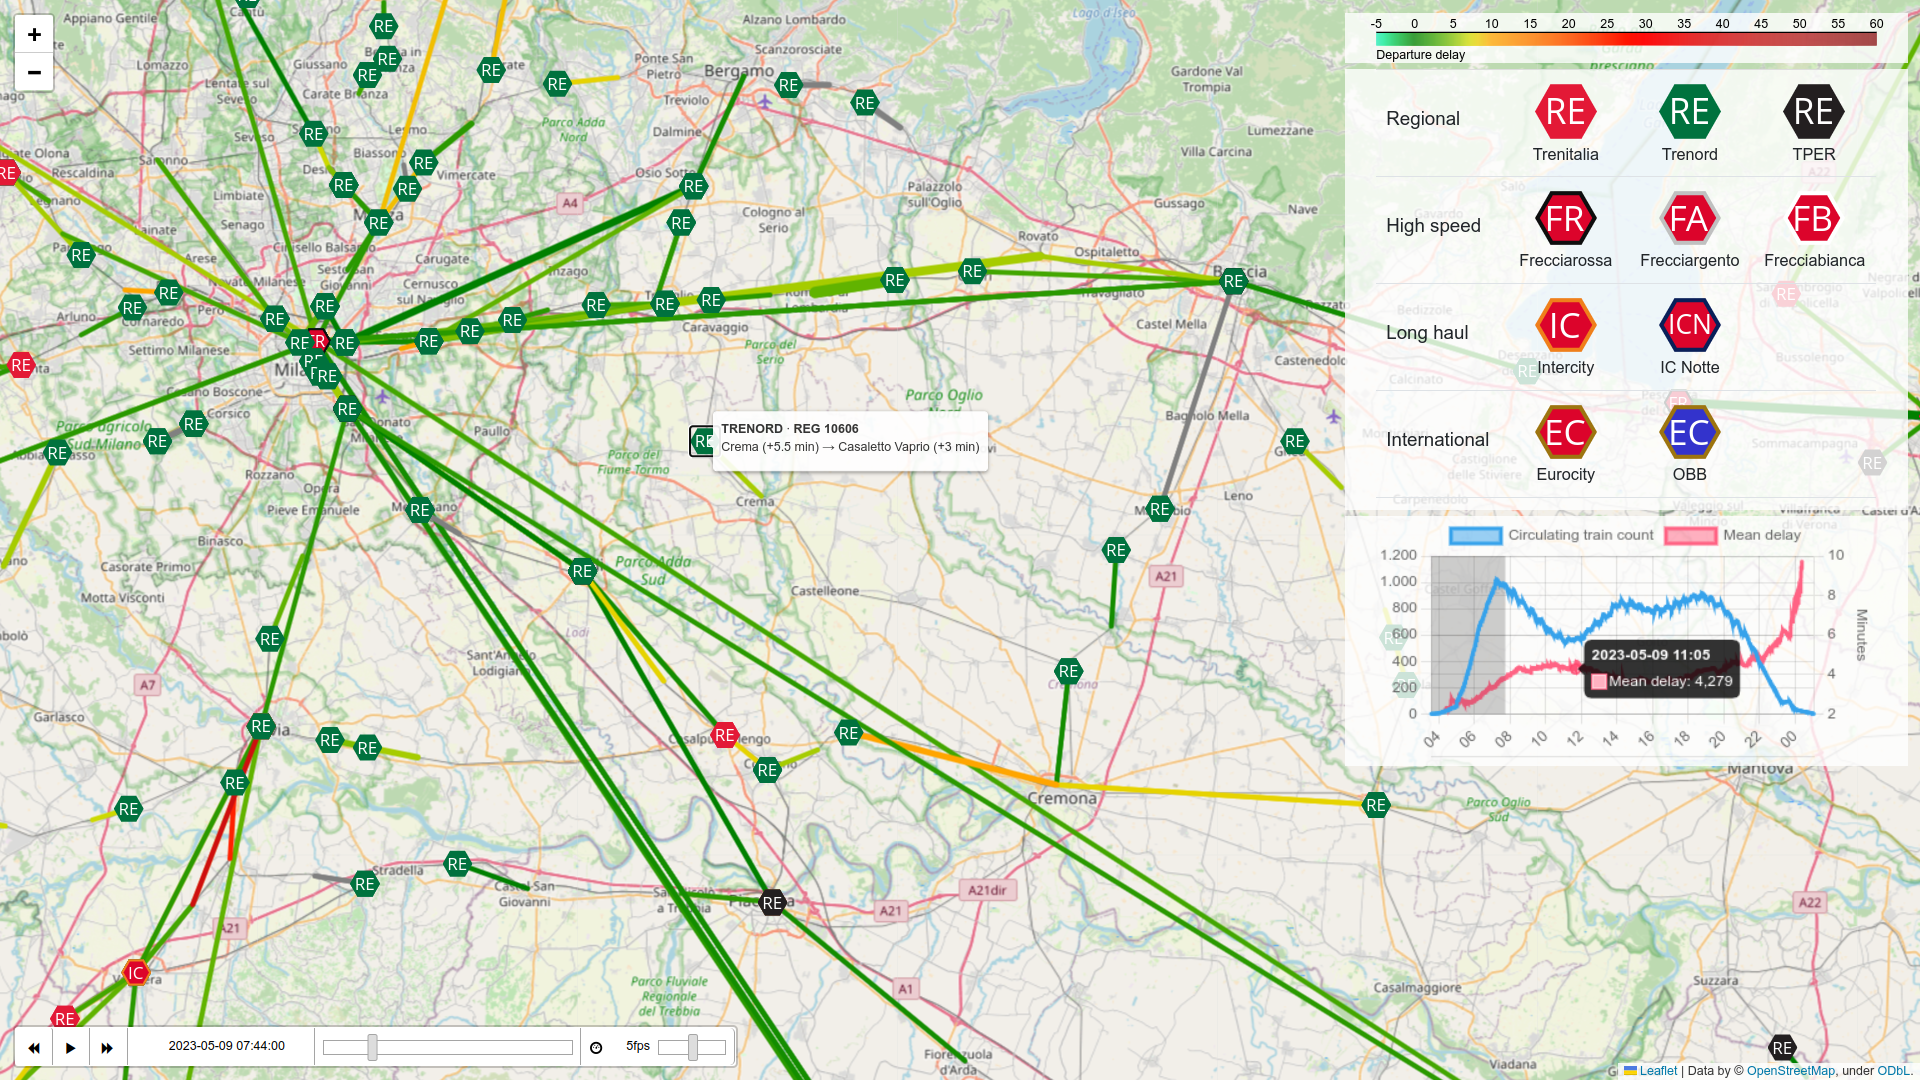
\includegraphics[width=1\textwidth]{images/trajectories_map.png}
    \caption{Dettaglio della mappa interattiva generata con i dati del
        09/05/2023}
\end{sidewaysfigure}

La mappa è \textbf{temporizzata}: con l'ausilio del selettore presente
in basso a sinistra è possibile \textit{avviare o fermare} il tempo,
\textit{scorrere} avanti e indietro e \textit{saltare} a un punto
specifico.  Il \textbf{contatore FPS}\footnote{\textit{Frames Per
        Second}, fotogrammi al secondo} permette di regolare la
\textit{velocità} dello scorrimento automatico del tempo.  In alto a
destra lo schermo è presente una \textbf{legenda} e un \textbf{grafico
    interattivo}, quest'ultimo con il \textbf{numero di treni
    circolati} il \textbf{ritardo medio di arrivo}.  L'\textbf{area
    grigia} in esso indica il periodo di tempo già visualizzato.
Spostando il cursore nell'area del grafico viene mostrato il
\textbf{valore puntuale}.  Nella mappa sono mostrate le
\textbf{tracce} dei treni in circolazione nell'istante considerato.
Ogni treno è rappresentato con una \textbf{\textit{testa}} e una
\textbf{linea colorata}: il colore e il simbolo della prima indicano
l'\textbf{impresa ferroviaria} e la \textbf{categoria} del treno, come
da legenda.  Il colore della linea rappresenta il \textbf{ritardo} e
il suo spessore l'\textbf{affollamento}\footnote{Dato presente solo
    per i treni Trenord}; essa connette la \textbf{fermata precedente}
con la successiva.  Spostando il cursore su una traccia vengono
mostrate le \textbf{informazioni sul treno} (come il numero e la
categoria) e \textbf{sulle fermate}.

La visualizzazione trasmette \textbf{a colpo d'occhio} l'andamento dei
treni, in particolare in corrispondenza dei punti nevralgici dei
grandi nodi ferroviari.  Il programma supporta i \textbf{filtri} già
precedentemente descritti, ma non raggruppamenti o aggregazioni.  A
causa dell'enorme quantità di informazioni i file HTML generati
possono essere di \textbf{notevoli dimensioni}, nell'ordine di
centinaia di megabyte.

\section{Altre analisi}
\label{altre_analisi}

Lo scopo di questa sezione è dimostrare tramite ulteriori analisi
approfondite le \textbf{forti potenzialità} dei dati raccoglibili con
lo strumento.  Si possono infatti progettare e calcolare nuovi
indicatori per meglio descrivere la \textit{reale} situazione attuale.
Ad esempio, è possibile pesare maggiormente le perturbazioni avvenute
in \textbf{ora di punta} secondo i tipici \textbf{flussi pendolari}
(trasferimento da piccola città a grande città la mattina e ritorno la
sera) oppure \textit{abbonare} i ritardi di pochi minuti nei viaggi a
\textbf{lunga percorrenza}.

È importante riconoscere che qualsiasi analisi può essere soggetta a
\textit{bias}, ma questi possono offrire una \textbf{diversa
    prospettiva} che contribuisce alla comprensione complessiva della
situazione.  Tra l'altro, neppure le \textbf{metriche ufficiali} ne
sono immuni: perché, ad esempio, l'indice di puntualità è spesso
calcolato come ``\textit{la percentuale di treni giunti a destino
    entro cinque minuti}''?  Perché non \textit{tre} o \textit{sette}?
Perché non sono contate le fermate intermedie?  Perché l'\textit{alta
    temperatura} estiva può essere considerata una \textit{causa di
    forza maggiore} e quindi esclusa?  Il trasporto pubblico si può
forse fermare se \textit{in estate fa caldo}?  L'autore non pretende
di stabilire in modo definitivo metriche e parametri, ma piuttosto
offre a chiunque la possibilità di trarre \textbf{le proprie
    conclusioni} scaricando i dati con lo strumento.

\subsection{Ritardo come variabile aleatoria}
\label{var_aleatoria}

\begin{figure}[p] \centering
    \subfloat[funzione di massa di
    probabilità~\protect{\cite[E]{StatJup}}]{
        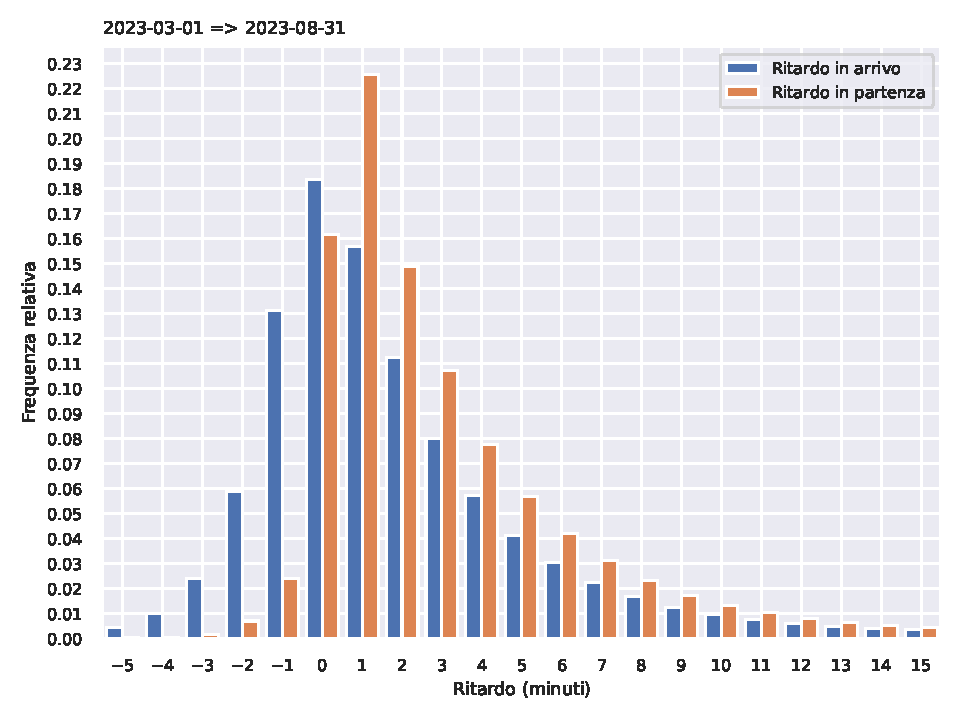
\includegraphics[width=0.95\textwidth]{images/delay_hist.pdf}
        \label{figure:delay_hist}
    } \vspace{5mm}
    \subfloat[funzione di ripartizione~\protect{\cite[F]{StatJup}}]{
        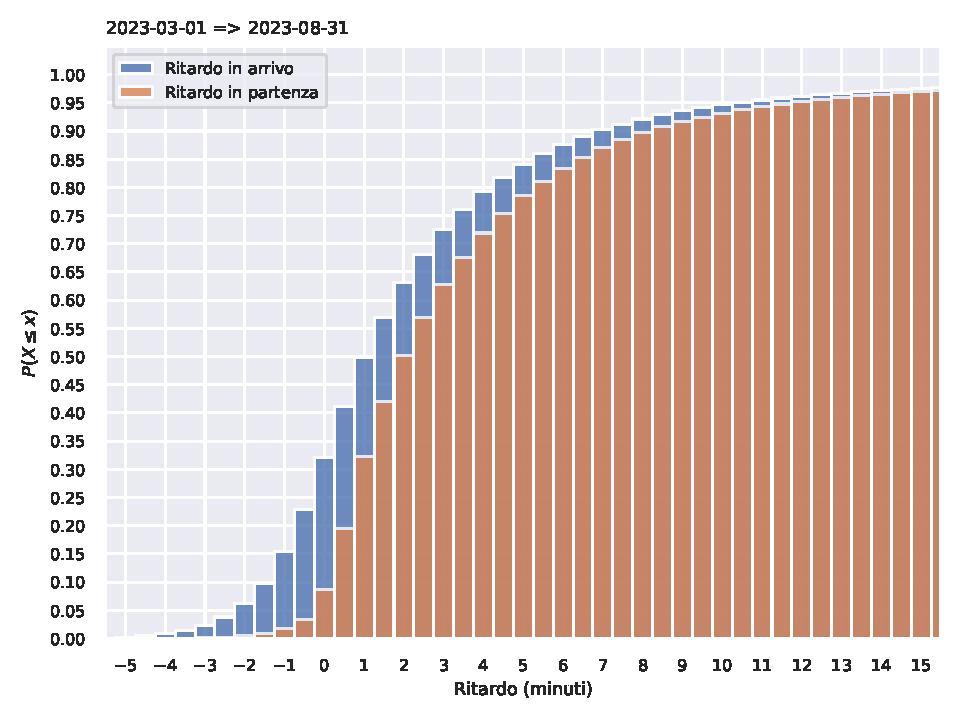
\includegraphics[width=0.95\textwidth]{images/delay_hist_acc.pdf}
        \label{figure:delay_hist_acc}
    }
    \caption{Distribuzione statistica dei ritardi dei treni italiani}
\end{figure}

In statistica, data una variabile aleatoria $X$ e una sua
specificazione $x$, si definisce una \textbf{funzione di massa di
    probabilità} $p_X(x)$ e una \textbf{funzione di ripartizione}
$F_X(x)$ rappresentanti rispettivamente la probabilità di una
particolare specificazione $P(X = x)$ o di $P(X \leq x)$.  Applicando
tali nozioni al dominio considerato, $X$ è la variabile aleatoria dei
ritardi, $p_X(x)$ la probabilità che \textit{un treno arrivi o parta
    da un fermata con $x$ minuti di ritardo} e $F_X(x)$ che \textit{un
    treno arrivi o parta da una fermata con al più $x$ minuti di
    ritardo}.  Il già citato \textbf{indice di puntualità} si può
semplificare con $F_X(5)$ dove $X$ considera solo le ultime fermate di
ogni corsa.

La \figurename~\ref{figure:delay_hist} approssima con un
\textbf{istogramma} la \textbf{funzione di massa di probabilità} dei
ritardi in arrivo e partenza.  Da sinistra, le due
\textbf{concentrazioni} di valori aumentano velocemente fino al valore
0 (\textit{treno in perfetto orario}) e 1 per poi decrescere
monotonicamente all'aumentare del ritardo con un decadimento
apparentemente esponenziale.  Intuitivamente, all'aumentare del
ritardo $x$, $p_X(x)$ (ovvero la probabilità che un treno arrivi o
parta con esattamente $x$ minuti di ritardo) diminuisce notevolmente.
La \figurename~\ref{figure:delay_hist_acc} approssima la già citata
\textbf{funzione di ripartizione}: ogni punto corrisponde a un
\textit{indice di puntualità} calcolato sui treni arrivati o partiti
da una fermata con un ritardo di $x$ minuti.  L'andamento è del tutto
equivalente alla visualizzazione precedente: solo il 72.20\% dei treni
arriva in fermata con al più 3 minuti di ritardo (standard Ferrovie
Federali Svizzere \cite{SbbPuntualita}), l'83.94\% con al più 5 e il
2.46\% con più di 20 minuti \cite[G]{StatJup}.

\subsection{Andamento infragiornaliero}
\label{andamento_infragiornaliero}

\begin{figure}[h]
    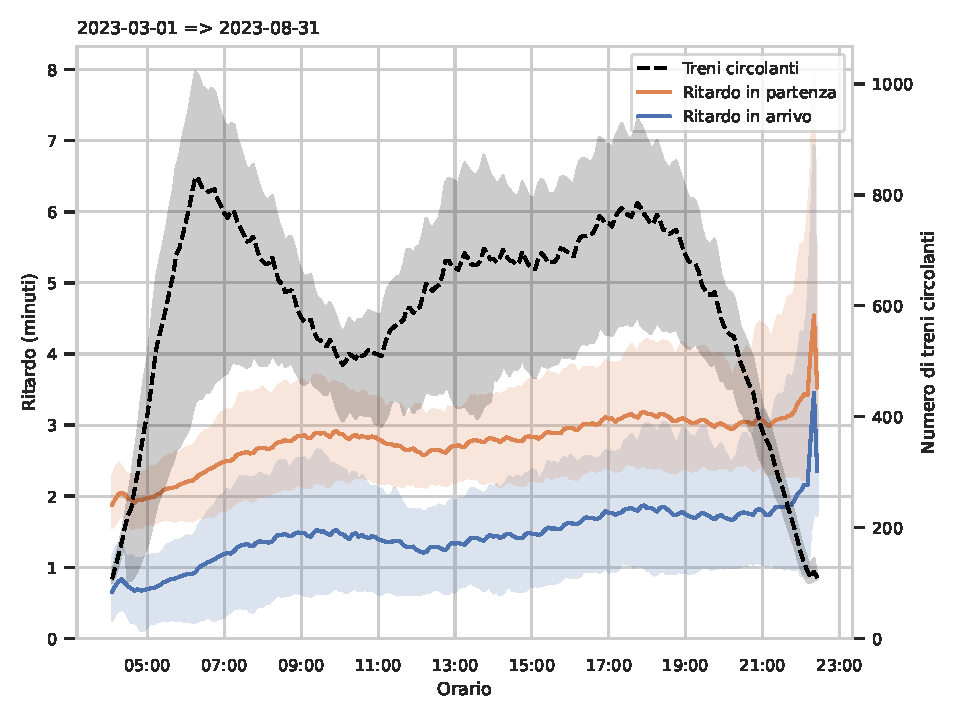
\includegraphics[width=1\textwidth]{images/intraday_delay.pdf}
    \caption{Andamento infragiornaliero dal 01/04/2023 al
        31/08/2023~\protect{\cite[H]{StatJup}}}
    \label{figure:intraday_delay}
\end{figure}

Con quest'analisi si vuole verificare una \textbf{correlazione} tra
l'orario della giornata, il numero di treni circolanti e il loro
ritardo.  La \figurename~\ref{figure:intraday_delay} è calcolata sui
\textbf{dati medi} di 5 mesi di rilevazioni: sull'ascissa sono
presenti gli \textbf{orari} di una giornata, sulle ordinate il
\textbf{ritardo} e il \textbf{numero di treni circolanti}.  Ad ogni
punto delle linee corrisponde il numero medio di treni circolanti o il
ritardo mediano dei treni in circolazione nell'orario
considerato\footnote{Un treno $x$ si dice \textit{in circolazione} in
    un tempo $t$ se e solo se
    $$\textsc{partenza}(x) \leq t <
    \textsc{arrivo}(x)$$ dove $\textsc{partenza}(x)$ e
    $\textsc{arrivo}(x)$ sono l'orario di partenza e arrivo
    dall'origine alla destinazione}.  Le aree di errore
(\textit{errorbar}) associate ad ogni serie includono il 95\%
percentile (2.5\% -~97.5\%) delle rilevazioni.  Riguardo il numero di
treni circolanti si può osservare dalla dimensione delle aree di
errore la sua \textbf{notevole varianza}, in particolare nella prima
fascia di punta (05:00 -~09:00) e nel pomeriggio.  La varianza dei
ritardi, benché anch'essa considerevole, rimane costante nel corso
della giornata.

L'andamento dei dati segue un \textbf{\textit{pattern} comune} in
tutte le giornate considerate: nelle ore di punta il numero di treni
aumenta notevolmente mentre diminuisce nella fascia 09:00 -~11:00, la
mattina presto e la sera tardi.  I \textbf{ritardi mediani} crescono
quasi costantemente all'aumentare delle ore, con una \textbf{lieve
    decrescita} tra le 10:00 e le 12:00.  Si ipotizza una
\textbf{correlazione positiva} tra il numero di treni e la
\textit{derivata prima} dei ritardi: l'effetto del traffico
ferroviario si propaga lentamente, ma è significativo.  Come si evince
anche numericamente in \figurename~\ref{figure:intraday_metrics},
dalle 21:00 il ritardo medio e la sua varianza aumenta velocemente,
forse a causa dal maggior rapporto di treni a lunga percorrenza
circolanti (spesso più \textit{ritardatari}).

\begin{figure}[h]
    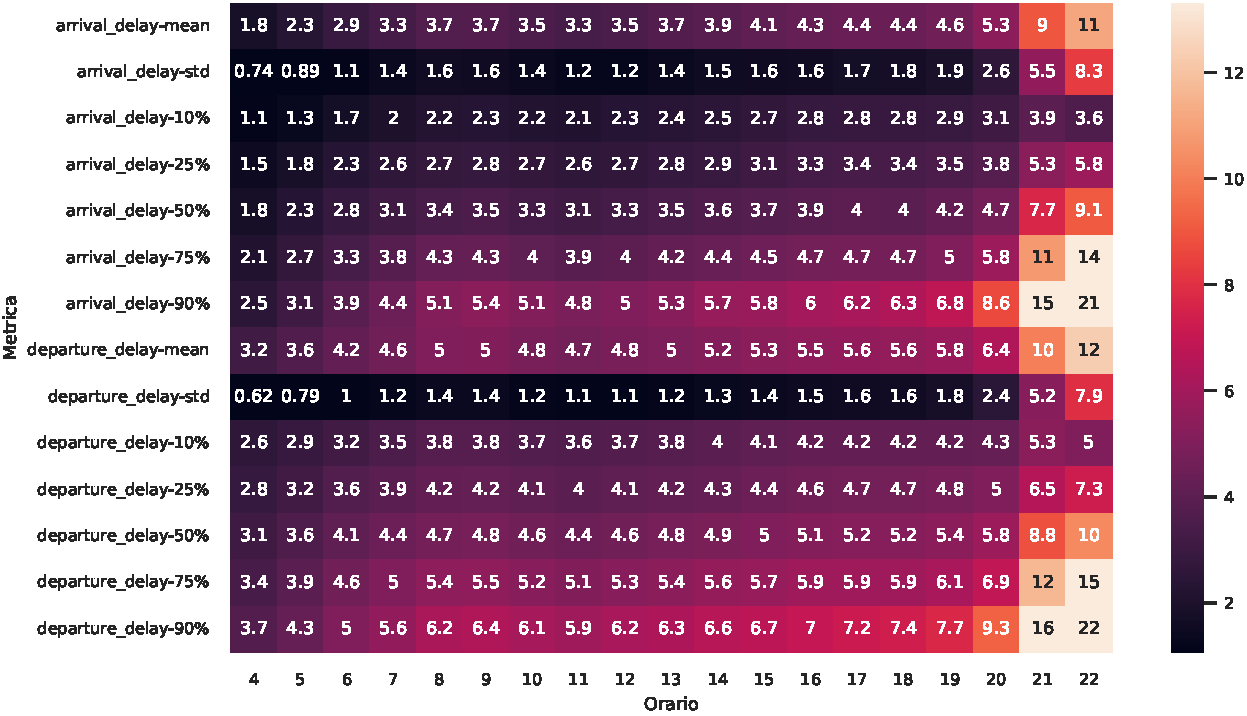
\includegraphics[width=1\textwidth]{images/intraday_metrics.pdf}
    \caption{Metriche infragiornaliere dal 01/04/2023 al
        31/08/2023~\protect{\cite[I]{StatJup}}}
    \label{figure:intraday_metrics}
\end{figure}

Al fine di mostrare solo dati significativi, in
\figurename~\ref{figure:intraday_delay}
e~\ref{figure:intraday_metrics} sono stati considerati per ogni
giornata \textbf{intervalli temporali} di 5 minuti con almeno 100
treni circolanti.  Con \textit{ritardo mediano di un intervallo
    temporale} si intende il valore mediano dei ritardi medi alle
fermate di ogni treno circolato nell'intervallo.

\subsection{Ritardo relativo}
\label{ritardo_relativo}

Nelle analisi precedenti il \textit{ritardo} è stato sempre inteso in
senso assoluto, senza considerare la \textit{durata} del viaggio.  In
\figurename~\ref{figure:delay_box_rc} è apparso evidente il maggiore
ritardo dei \textbf{treni a lunga percorrenza}, aventi per l'appunto
una durata maggiore.

Per \textit{ritardo relativo di una corsa} si intende il rapporto tra
il suo \textit{ritardo assoluto mediano} e la sua \textit{durata},
intesa come la differenza tra l'orario di partenza programmato della
prima fermata e l'orario di arrivo all'ultima fermata.  In
\figurename~\ref{figure:delay_box_percentage_wd} sono graficati i
\textit{boxplot} dei \textit{ritardi relativi} delle corse di ogni
impresa ferroviaria.  Il \textit{trend} è opposto rispetto a quanto
osservato in \figurename~\ref{figure:delay_box_rc}: le imprese
ferroviarie a \textbf{lunga percorrenza} hanno un \textit{ritardo
    assoluto} maggiore, ma un \textit{ritardo relativo} minore.  Tra
le imprese regionali, la \textbf{peggiore rimane Trenord} (ritardo
medio in partenza 6.16\%), seguita da \textbf{Tper} (5.62\%) e
\textbf{Trenitalia} (4.90\%).

I dati precedenti suggeriscono una \textbf{intuitiva correlazione
    lineare} tra la \textit{durata del viaggio} e il \textit{ritardo
    assoluto mediano}.  In
\figurename~\ref{figure:delay_duration_corr} è mostrata una
\textbf{regressione lineare} tra il ritardo mediano assoluto della
corsa e la sua durata.  Ad ogni punto nel piano corrisponde un
\textit{50-quantile}\footnote{Il campione è diviso in 50 segmenti di
    durate aventi la medesima dimensione} delle durate e la
\textit{media} dei \textit{ritardi mediani} delle corse.  La
correlazione è evidente: escludendo i valori dei quantili più estremi,
l'\textbf{andamento} è prevalentemente \textbf{lineare}.
All'aumentare della durata della corsa, il ritardo tendenzialmente
aumenta.

\begin{figure}[h]
    \centering
    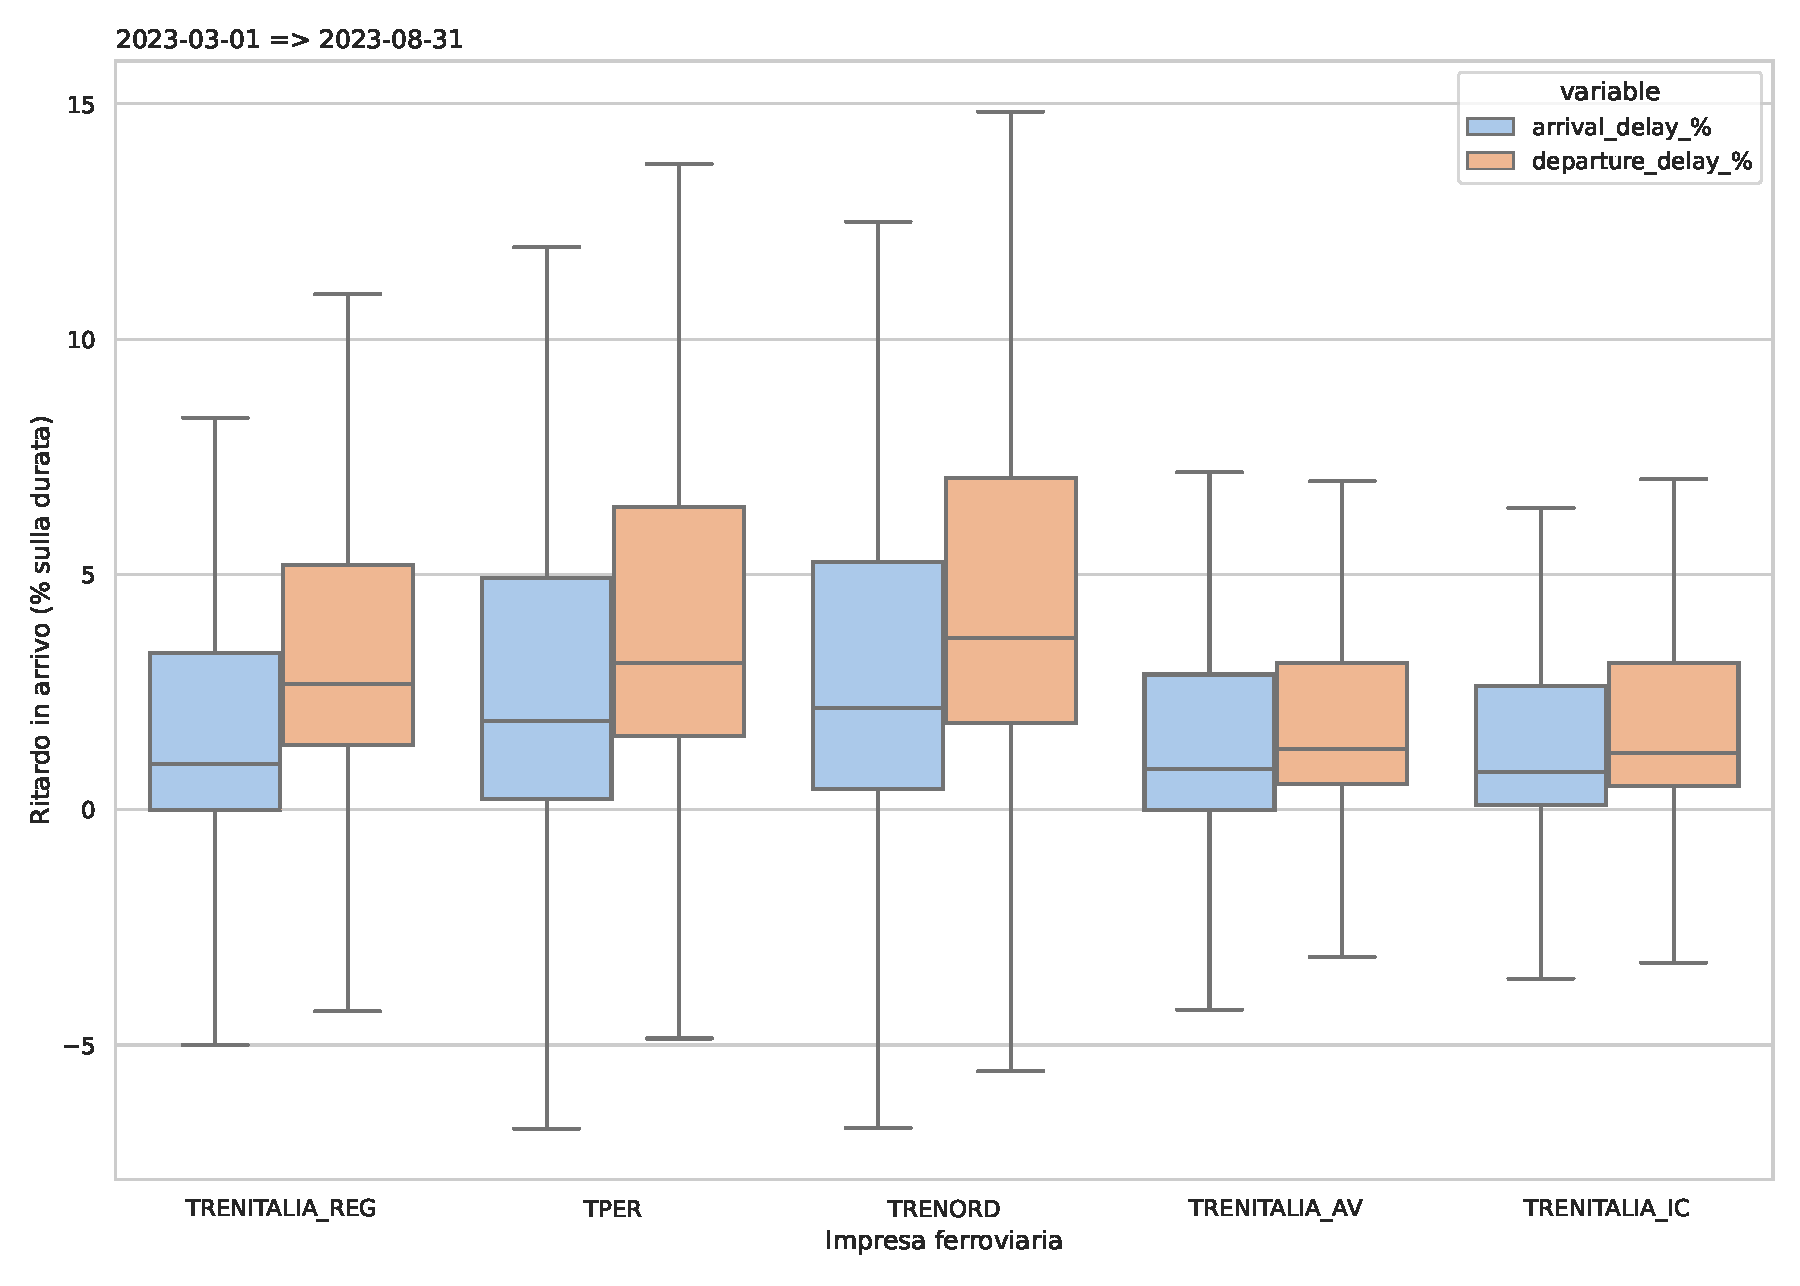
\includegraphics[width=1\textwidth]{images/delay_box_percentage_wd.pdf}
    \caption{\textit{Ritardo relativo} dei treni italiani, per impresa
        ferroviaria~\cite[J]{StatJup}}
    \label{figure:delay_box_percentage_wd}
\end{figure}

\begin{sidewaysfigure}[p]
    \centering
    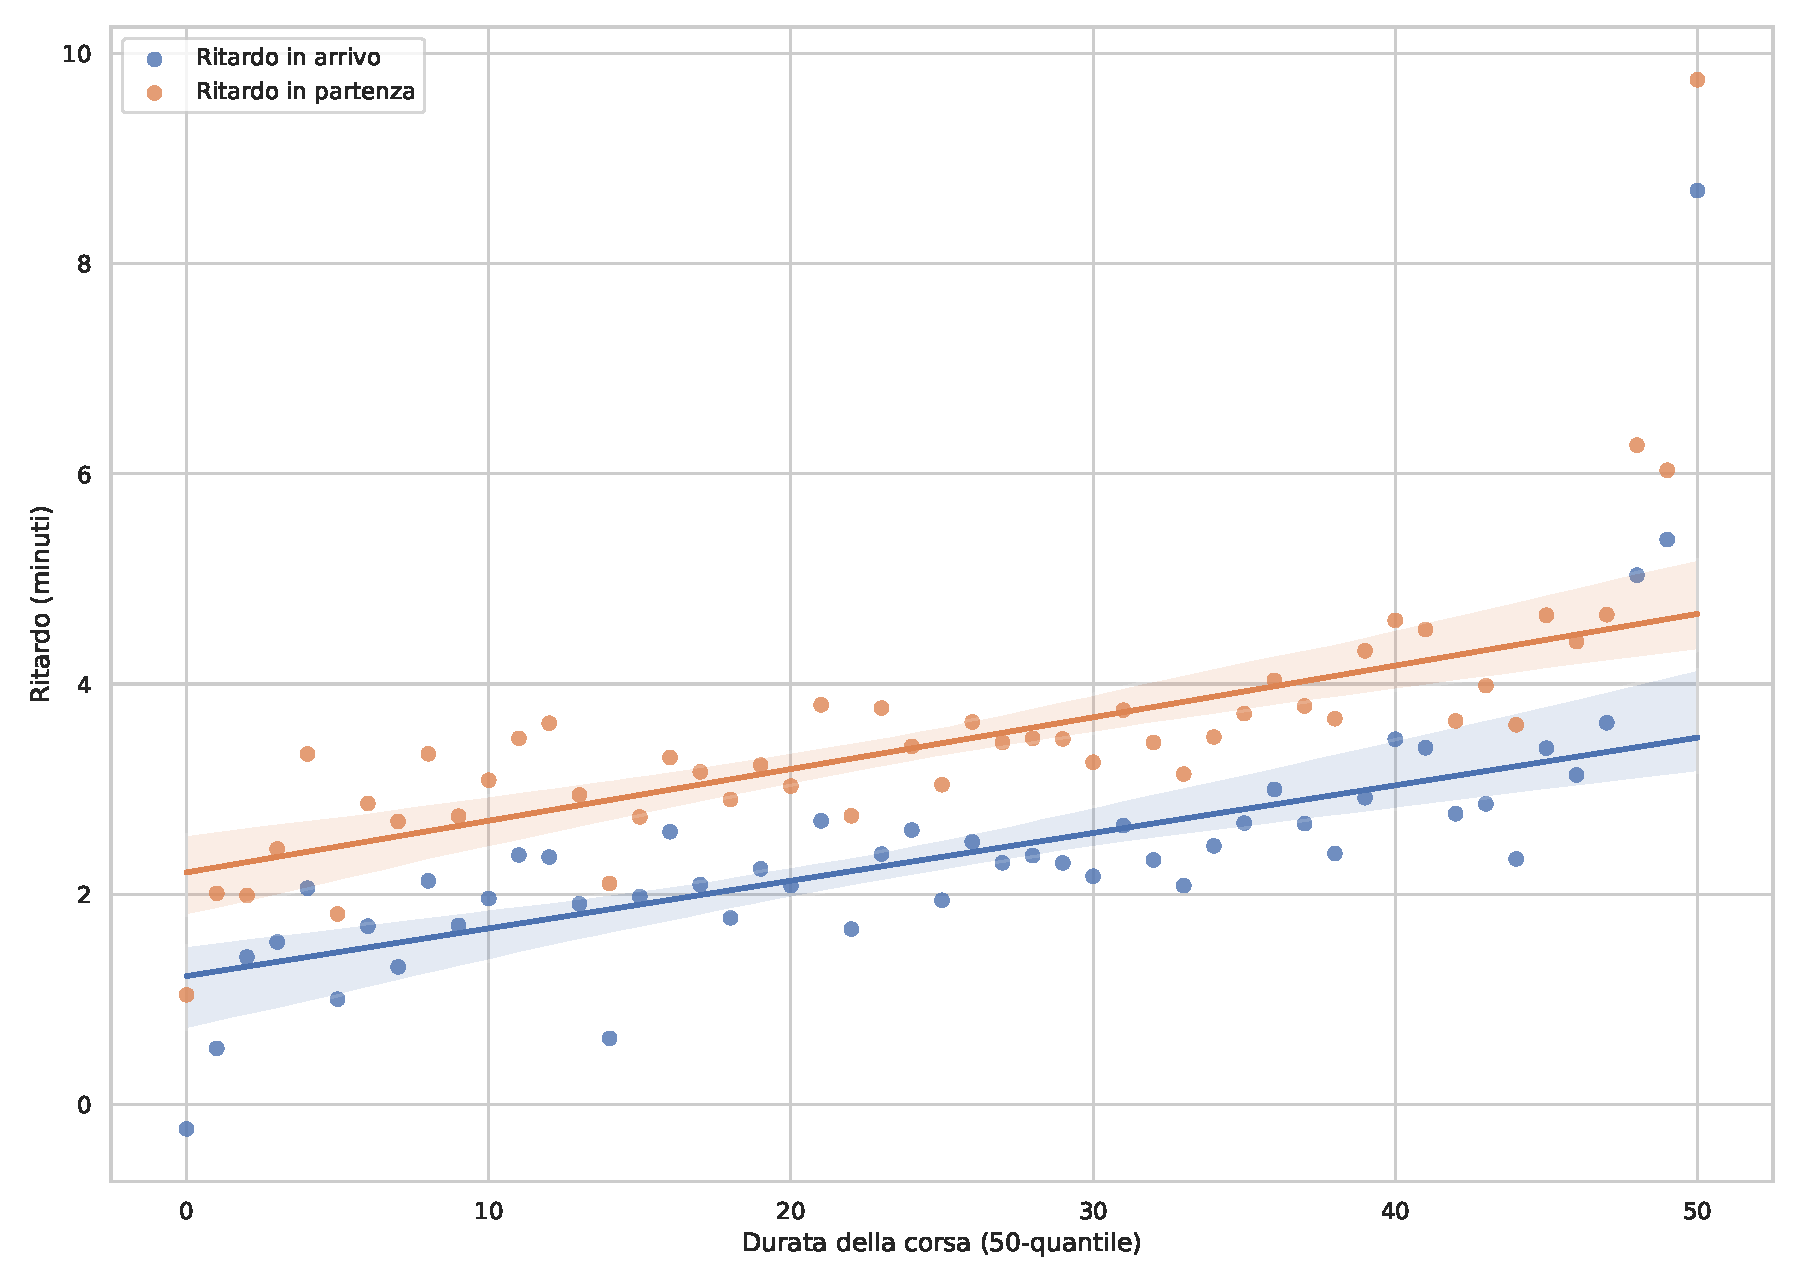
\includegraphics[width=1\textwidth]{images/delay_duration_corr.pdf}
    \caption{Correlazione tra ritardo mediano assoluto di una corsa e
        durata~\cite[K]{StatJup}}
    \label{figure:delay_duration_corr}
\end{sidewaysfigure}

\chapter{Conclusioni}

Il lavoro di Tesi si conclude con \textbf{risultati soddisfacenti},
nonostante molte questioni rimangano ancora oggetto di discussione.
% Si ricorda che l'\textbf{obiettivo principale} del lavoro di Tesi
% \textit{non} è stata l'analisi dei dati raccolti, ma l'attività di
% \textit{raccolta} stessa.  \todo{AT: vero fino ad un certo punto,
%     diciamo che è stata la raccolta e la proposta di estrazione di
%     alcune statistiche suggerenti l'utilità del processo}
Dopo aver descritto le \textbf{principali
    Società} (\S~\ref{societa_territorio}), la differenza tra
\textbf{servizio pubblico} e \textbf{offerte a mercato}
(\S~\ref{servizio_pubblico}) e il complesso meccanismo della
\textbf{performance regime} (\S~\ref{performance_regime}), è stata
mostrata e parzialmente documentata (\S~\ref{documentazione})
l'\textbf{infrastruttura tecnologica} sfruttata ai fini del progetto
(\S~\ref{infrastruttura_tecnologica}).  Nonostante le
\textit{notevoli} incogruenze, la relativa semplicità delle
\textbf{API} di Viaggiatreno e Trenord e l'assenza di
\textit{rate-limit} o autenticazione hanno consentito di
\textbf{scaricare ininterrottamente} considerevoli quantità di
informazione durante i mesi tra aprile e agosto 2023.

In \S~\ref{panorama_giuridico} è stato fornito un ampio resoconto del
\textbf{panorama giuridico, politico e legislativo} con diverse
riflessioni sulla legittimità dell'uso dei dati.  Il \textbf{caso
    Trenìt} (\S~\ref{caso_trenit}) è emblematico: le richieste di
Trenitalia hanno portato alla temporanea sospensione di
un'applicazione utilizzata da migliaia di viaggiatori ogni giorno, per
\textit{aver utilizzato dati altrui}.  Il \textbf{dato}, nella sua più
\textit{innocente oggettività}, è conteso: può davvero una
\textit{impresa pubblica}, titolare di contratti di \textit{servizio
    pubblico} con \textit{enti pubblici} vantare diritti esclusivi
sulle \textbf{informazioni in tempo reale} della circolazione
ferroviaria?  La risposta del Tribunale è un debole \textit{no},
basato più su tecnicismi legati alla definizione di \textit{banca
    dati} e \textit{parte sostanziale} che sul diritto civico di
\textbf{conoscere} e \textbf{controllare} l'operato
dell'Amministrazione.

A tale proposito, sono state inoltrate due istanze di \textbf{accesso
    civico generalizzato} (\S~\ref{foia}): una al Ministero dei
Trasporti per Trenitalia e una a Regione Lombardia per Trenord.  Il
risultato della prima è stato un \textbf{diniego totale}, giustificato
dalla \textit{tutela degli interessi commerciali} dell'impresa.  I
dati richiesti sui ritardi, infatti, sono accorpati con quelli sulla
occupazione dei posti a sedere e valore economico delle corse.
Dovendo Trenitalia competere con altre imprese ferroviarie e servizi
di trasporto a lunga percorrenza (come Italo), il diniego è stato
ritenuto \textit{ragionevole} dall'Autore.  Regione Lombardia, d'altra
parte, ha risposto con un \textbf{dinego parziale}, fornendo tra le
altre cose alcuni \textit{report} su ritardi e cancellazioni di tutte
le direttrici.  Quest'ultimi hanno ancora una volta evidenziato la
fondamentale importanza dei \textbf{dati disaggregati}: per via della
rilevata \textbf{forte disomogeneità} di \textit{performance} tra
direttrici (\figurename~\ref{figure:lomb_heatmap}), i dati pubblicati
sul sito web (\figurename~\ref{lombardia_puntualita}) sono da
considerarsi \textbf{quasi irrilevanti}.  L'accesso ai \textbf{dati
    grezzi}, tutt'ora non contemplato, porterebbe ad un livello di
dettaglio tale da consentire la \textbf{totale comprensione} della
situazione ai Cittadini più curiosi o politicamente interessati.  Le
richieste di chiarimento sui disservizi, i dati relativi alla
frequentazione, posti offerti e i \textit{report} sui costi sostenuti
sono state oggetto di \textbf{diniego}, cui ragioni non sono state
nemmeno accuratamente documentate.  Spetta al lettore il compito di
valutare il comportamento dell'Amministrazione, anche alla luce del
\textbf{pesante conflitto di interesse} che vede la Regione vestirsi
del ruolo di \textit{appaltatore} e \textit{appaltante} del medesimo
servizio.

Nel secondo capitolo (cap.\@~\ref{progettazione}) è stata descritta la
progettazione e l'implementazione dei software prodotti durante il
lavoro di Tesi: lo \textit{scraper} (\S~\ref{scraper}),
l'\textit{extractor} (\S~\ref{extractor}) e l'\textit{analyzer}
(\S~\ref{analyzer}).  Il primo si occupa di scaricare con un
\textbf{algoritmo di salvataggio incrementale} (\S~\ref{alg_scraping})
le informazioni \textit{real-time} della circolazione ferroviaria, il
secondo \textbf{converte} quanto salvato in comodi file CSV e l’ultimo
propone delle \textbf{analisi predefinite} e
\textbf{parametrizzabili}.  Tutti gli strumenti sono scritti in
Python, sono \textit{open-source} e sono utilizzabili da linea di
comando.  Per la prima volta è disponibile una \textit{suite} di
strumenti utile a \textbf{scaricare}, \textbf{convertire} e
\textbf{analizzare} in modo indipendente i dati della circolazione
ferroviaria italiana.

Per più di 5 mesi, in una macchina del \textit{Dipartimento di
    Informatica} dell'Università degli Studi di Milano, un'istanza
dello \textit{scraper} ha campionato informazioni dettagliate su più
di 10 milioni \textit{eventi fermata-treno}.  Il \textit{bottino} è
notevole non solo dal punto di vista statistico, ma anche
\textbf{politico}: non sono mai stati ufficialmente pubblicati dati
così specifici e \textit{densi} di informazione, nemmeno nella
virtuosa Emilia Romagna.  Nell'ultimo capitolo (cap.\@~\ref{analisi})
sono state proposte alcune analisi e visualizzazioni, in parte
generate con lo strumento e in parte costruite \textit{ad-hoc}.
Quest'ultime sono puntualmente \textbf{riproducibili} eseguendo il
\textit{notebook} citato~\cite{StatJup}.  In pochi passi è stato
possibile generare semplici statistiche descrittive
(\S~\ref{stat_describe}) e osservare come generalmente i \textbf{treni
    recuperano ritardo} sostando in una fermata.  In
\S~\ref{stat_delay_boxplot} sono stati analizzati i
\textbf{\textit{boxplot} dei ritardi} raggruppati per impresa
ferroviaria e giorno della settimana.  Oltre alla curiosa
\textit{maggiore puntualità} delle corse circolanti nel weekend, sono
state rilevate notevoli differenze tra le imprese ferroviarie
regionali e quelle a lunga percorrenza (approfondite successivamente
in \S~\ref{ritardo_relativo}).  Anche il \textbf{numero di treni}
varia nel weekend (\S~\ref{stat_day_train_count}): in particolare, il
numero di corse regionali Trenitalia e Tper dimunisce notevolmente.

Nell'ambito del lavoro di Tesi è stato necessario definire
puntualmente il \textbf{concetto di \textit{linea ferroviaria}}
avvalendosi delle sole informazioni a disposizione
dell'\textit{analyzer} (\S~\ref{linee_ferroviarie}).  Con questa
nozione è possibile produrre i c.d.\@ ``\textit{orari grafici}''
(\S~\ref{stat_timetable}) di una linea per visualizzare tutti le corse
effettivamente circolate in una giornata.  Un'altra visualizzazione in
grado di offrire una ``visione di insieme'' è la \textbf{mappa
    temporizzata} (\S~\ref{stat_trajectories_map}): ogni treno è
rappresentanto da una \textit{linea colorata} avente come
\textit{testa} un poligono indicante la categoria della corsa.

Le \textbf{ultime analisi} hanno cercato di meglio descrivere
attraverso ulteriori visualizzazioni la \textit{reale situazione}.
Modellare il \textit{ritardo} come una \textbf{variabile aleatoria}
(\S~\ref{var_aleatoria}) ha permesso di esprimere l'\textit{indice di
    puntualità} come la sua \textit{funzione di ripartizione},
permettendo di affermare che solo l'83.94\% dei treni arriva con al
più 5 minuti di ritardo.
% \todo{AT: non sono andato indietro a controllare, invece il loro claim sui 5 minuti era veritiero?}
Concentrando i dati raccolti nei mesi in una
sola giornata si ottiene l'\textbf{andamento infragiornaliero}
(\S~\ref{andamento_infragiornaliero}): intuitivamente, nelle
\textit{ore di punta} circolano più treni.  Si ipotizza inoltre una
\textbf{correlazione} tra il numero di treni circolanti e la
\textit{derivata prima} del ritardo.  Sulla \textit{falsa riga} di
questa ipotesi, viene introdotto il concetto di \textbf{ritardo
    relativo} (\S~\ref{ritardo_relativo}) legato alla \textit{durata}
della corsa.  I risultati sono sorprendenti: le imprese ferroviarie a
lunga percorrenza sono risultate \textit{relativamente più puntuali}
delle colleghe regionali, nonostante siano \textit{assolutamente più
    in ritardo}.  La \textit{performance} mediana di \textbf{Trenord}
si conferma essere la peggiore nell'ambito del trasporto regionale,
seguita da Tper e Trenitalia.  Infine, è stata dimostrata una
intuitiva \textbf{correlazione lineare} tra il \textit{ritardo
    assoluto} di una corsa e la sua durata.

\section*{Sviluppi futuri}

L'argomento è tutt'altro che \textit{esaurito}.  Gli eventuali
\textbf{obblighi di Legge} (anche comunitaria) riguardo l'accesso e la
pubblicità dei dati in possesso delle imprese ferroviarie è ancora
oggetto di discussione: \textit{può davvero essere così difficile
    accedere ad informazioni tanto banali come l'orario effettivo di
    arrivo di un treno?}

La \textit{suite} di strumenti può essere utilizzata come base di
partenza per \textbf{ulteriori analisi}, anche complesse.  Ad esempio,
si potrebbe \textbf{modellare l'intera rete ferroviaria} e trovare le
tratte più bisognose di interventi di potenziamento.  Oppure,
implementare con tecniche di intelligenza artificiale un
\textbf{predittore di ritardi} che, dato lo stato corrente della
circolazione ferroviaria, condizioni ambientali e periodo stagionale,
comunica al viaggiatore con una certa confidenza con quanto ritardo
arriverà il treno o la probabilità di riuscire prendere una
coincidenza.

L'\textbf{accesso ai dati} è \textit{\textbf{condizione necessaria}}
per un dialogo serio e costruttivo sul trasporto ferroviario italiano
ed è una \textit{cartina di tornasole} della Trasparenza della nostra
Democrazia.

\vfill

\epigraph{Dove un superiore pubblico interesse non imponga un
    momentaneo segreto, la casa dell'amministrazione dovrebbe essere
    di vetro.}{\textit{Filippo Turati}\\17 giugno 1908,~\cite{Turati}}

% -----------------------------------------------------------------

\printbibliography

\addcontentsline{toc}{chapter}{Bibliografia}

\appendix

\chapter{Documentazione}
\label{documentazione}

\section{Terminologia}
\label{terminologia}

Prima di analizzare le API occorre fissare alcuni termini e concetti
fondamentali, sorprendentemente spesso controintuitivi.

Una \textbf{stazione} è un \textit{luogo di sosta temporanea} per i
convogli ferroviari.  Ha un \textit{nome} e uno o più \textit{codici}
corrispondenti, utilizzati per identificarla.  I nomi delle stazioni
non necessariamente rispettano i nomi delle località in cui sono
situate e una città può naturalmente includere più stazioni.  In
alcuni casi l'API ritorna ``stazioni'' non più attive o inesistenti,
come posti di movimento o depositi ferroviari.

Con il termine \textbf{treno} si intende la \textit{corsa di un
    convoglio ferroviario}.  I treni che non fanno servizio
viaggiatori sono oltre gli obiettivi del progetto.  Ogni treno ha una
\textit{numero}, una \textit{origine}, una \textit{destinazione}, una
collezione ordinata di \textit{fermate intermedie} e altre proprietà
che verranno approfondite nei prossimi capitoli.  Il numero di treno
non è un \textbf{identificatore univoco} e non può essere utilizzato
come tale, in quanto può essere riassegnato a treni di altre imprese
ferroviarie.  La stessa \textit{corsa} può variare tra giornate
diverse, sia per motivi programmati (per esempio, fermate
straordinarie nel weekend) che non (treni parzialmente soppressi).  Un
treno è univocamente identificato dalla tripla
$(\texttt{Data}, \, \texttt{Origine}, \, \texttt{Numero})$.

Una \textbf{fermata} è una stazione in cui un treno, oltre che a
transitare, \textit{sosta}.  L'\textit{origine} e la
\textit{destinazione} sono considerarsi fermate particolari: un treno
sosta quindi in almeno due fermate, la prima e l'ultima.  Ad ogni
fermata è associato un \textit{orario programmato} ed
\textit{effettivo} di arrivo e partenza la cui differenza è il
relativo ritardo.  La prima fermata non può avere un orario di arrivo
e viceversa.  Le fermate possono essere ordinarie, straordinarie o
soppresse.  Un treno avente alcune fermate sorppresse è detto
\textit{parzialmente soppresso}, uno con tutte \textit{soppresso}.

\section{API di Viaggiatreno}

Le API di Viaggiatreno (vedi \S~\ref{viaggiatreno}) non dispongono di
una documentazione ufficiale e non sono conformi alla architettura
REST o ad altri standard \textit{de facto} \cite{Giunta}.  Numerosi
tentativi sono stati fatti dalla comunità open source italiana per
documentarle: in particolare si ringraziano Stefano (sabas)
\cite{Sabas}, Luca Grandi \cite{Grandi} e Fabrizio Tarizzo
\cite{Tarizzo} per il loro fondamentale contributo.  I metodi sono
generalmente accessibili al percorso
\texttt{/infomobilita/\-resteasy/\-viaggiatreno/\-$M$/\-$P_1$/\-$P_2$/\-$\dots$/\-$P_n$}
dove $M$ è il nome del metodo e $P_1, P_2, \dots, P_n$ i suoi
parametri. A seconda della richiesta l'API può rispondere in JSON o in
altri formati \textit{plain text}.


\subsection{\texttt{/cercaStazione/<nome>}}
\label{cercaStazione}

Il metodo ritorna \textit{tutte le stazioni} cui nome inizia con il
nome indicato.  Per ogni stazione viene ritornato il suo codice, un
nome ``lungo'' e uno ``breve'' e il nome della città in cui si trova.

\subsubsection{Esempio}

$\Rsh$ \texttt{/cercaStazione/MILANO}
\begin{minted}[fontsize=\footnotesize]{js}
[
  {
    "nomeLungo": "MILANO CENTRALE", // nome lungo
    "nomeBreve": "Milano Centrale", // nome breve (può essere nullo)
    "label": "Milano",              // città (può essere nullo)
    "id": "S01700"                  // codice stazione
  },
  // ...
]
\end{minted}

\subsubsection{Avvertenze}

Il metodo non restituisce tutte le stazioni.  Ad esempio, la stazione
di Arcene (BG) non viene mai ritornata, neanche cercandola dal sito
web.  L'unico modo per reperire il suo ID è consultare le fermate di
un treno in corsa.

\subsection{\texttt{/regione/<codiceStazione>}}

Il metodo ritorna il codice della regione di appartenza della stazione
richiesta.  Il contenuto della risposta, in testo semplice, può essere
utilizzato nel metodo successivo.

\begin{table}[h] \centering
    \begin{tabular}{r|l}
      Codice & Nome \\
      \hline
      1 & Lombardia \\
      2 & Liguria \\
      3 & Piemonte \\
      4 & Valle D'Aosta \\
      5 & Lazio \\
      6 & Umbria \\
      7 & Molise \\
      8 & Emilia Romagna \\
      9 & Trentino-Alto Adige \\
      10 & Friuli Venezia Giulia \\
      11 & Marche \\
    \end{tabular}
    \begin{tabular}{r|l}
      Codice & Nome \\
      \hline
      12 & Veneto \\
      13 & Toscana \\
      14 & Sicilia \\
      15 & Basilicata \\
      16 & Puglia \\
      17 & Calabria \\
      18 & Campania \\
      19 & Abruzzo \\
      20 & Sardegna \\
      21 & Trentino-Alto Adige \\
      22 & Trentino-Alto Adige
    \end{tabular}
    \caption{Codici API delle regioni italiane}
    \label{regioni}
\end{table}

\subsubsection{Esempio}

$\Rsh$ \texttt{/regione/S01700} \hfill (Milano Centrale)
\begin{minted}{text}
1
\end{minted}

\subsubsection{Avvertenze}

Osservando la Tabella~\ref{regioni} si può notare che le stazioni
della regione Trentino-Alto Adige assumono 3 codice regione
differenti, senza nessun pattern apparente.  Non tutte le stazioni
sono riconosciute, specialmente quelle in gestione a Ferrovienord.  In
tal caso, la risposta dell'API è \texttt{0}.

\subsection{\texttt{/elencoStazioni/<codiceRegione>}}
\label{elencoStazioni}

Il metodo ritorna tutte le stazioni della regione data.  Con il codice
\texttt{0} vengono ritornate solo le stazioni principali.  La
funzionalità è presumibilmente utilizzata per popolare la mappa
presente in homepage.

La risposta è in formato JSON e per ogni elemento viene fornito un
superinsieme di informazioni rispetto a \texttt{cercaStazione}, come
la latitudine e longitudine.

\subsubsection{Esempio}

$\Rsh$ \texttt{/elencoStazioni/3} \hfill (Piemonte)
\begin{minted}[fontsize=\footnotesize]{js}
[
 {
    "codReg": 3,  // Codice regione
    "tipoStazione": 3,
    "dettZoomStaz": [  // (può non essere presente)
      {
        "codiceStazione": "S01013",
        "zoomStartRange": 8,
        "zoomStopRange": 9,
        "pinpointVisibile": true,
        "pinpointVisible": true,
        "labelVisibile": true,
        "labelVisible": true,
        "codiceRegione": null
      },
      {
        "codiceStazione": "S01013",
        "zoomStartRange": 10,
        "zoomStopRange": 11,
        "pinpointVisibile": true,
        "pinpointVisible": true,
        "labelVisibile": true,
        "labelVisible": true,
        "codiceRegione": null
      }
    ],
    "pstaz": [],
    "mappaCitta": {
      "urlImagePinpoint": "",
      "urlImageBaloon": ""
    },
    "codiceStazione": "S01013",
    "codStazione": "S01013",
    "lat": 45.943821,  // Latitudine (può essere nullo)
    "lon": 8.47224,  // Longitudine (può essere nullo)
    "latMappaCitta": 0,
    "lonMappaCitta": 0,
    "localita": {  // Medesime proprietà di cercaStazione
      "nomeLungo": "VERBANIA-PALLANZA",
      "nomeBreve": "Verbania",
      "label": "Verbania-Pallanza",
      "id": "S01013"
    },
    "esterno": false,
    "offsetX": -4,
    "offsetY": 10,
    "nomeCitta": "Verbania"  // Vedere avvertenze
  }, ...
]
\end{minted}

\subsubsection{Avvertenze}

Il campo \texttt{nomeCitta} può essere nullo oppure ``\texttt{A}''
(stesso significato).  Sono generalmente ritornate più stazioni
rispetto a \texttt{cercaStazione}, ma comunque non tutte: le stazioni
senza informazioni sulla localizzazione, come Aiello (UD), sono
ignorate \textit{in toto}.  Alcune ``stazioni'' sono punti di appoggio
per generare la mappa e sono da ignorare: si distinguno in quanto
hanno \texttt{tipoStazione} uguale a ``\texttt{4}''.  Infine, esistono
stazioni figuranti in più regioni contemporaneamente: per esempio, la
stazione di Casalmaggiore (CR) risulta essere sia in Lombardia che in
Emilia Romagna.  Verificando con \texttt{/regione}, però, la stazione
risulta correttamente in Lombardia.

\subsection{\texttt{/<partenze|arrivi>/<orarioAttuale>}}
\label{partenzeArrivi}

I metodi \texttt{partenze} e \texttt{arrivi} ritornano i treni in
partenza o in arrivo della stazione data.  Il campo
\texttt{orarioAttuale} è da indicare nel formato \texttt{\%a \%b \%d
    \%Y \%H:\%M:\%S \%Z\%z} e non può essere diverso dall'orario in
cui si invia la richiesta.

La risposta è in formato JSON e contiene molte informazioni sia sul
treno che sulla \textit{fermata} nella stazione richiesta.

\subsubsection{Esempio}

$\Rsh$ \texttt{/partenze/S01700/Wed Mar 08 2023 17:04:00 GMT+0100}
\hfill (Milano Centrale) \\

\noindent \textit{La risposta è nello stesso formato degli elementi
    dell'array \texttt{fermate} documentato con il metodo
    \texttt{andamentoTreno} (\ref{andamentoTreno}) --- è quindi stata
    omessa.}

\subsection{\texttt{/cercaNumeroTrenoTrenoAutocomplete/<numeroTreno>}}
\label{trenoAutocomplete}

Come detto precedentemente (\ref{terminologia}), un treno è
univocamente identificabile dalla combinazione del suo numero, origine
e data di partenza.  Il metodo
\texttt{cerca\-Numero\-Treno\-Treno\-Autocomplete} serve per
disambugare treni aventi lo stesso numero, ritornando il codice della
stazione di origine e il
\textit{timestamp}\footnote{\label{timestamp}Tutti i timestamp
    dell'API di Viaggiatreno sono intesi come \textit{numero di
        \textbf{millisecondi} passati dal 1° gennaio 1970}, nel fuso
    orario locale.} della mezzanotte del giorno di partenza della
corsa.

La risposta è in \texttt{text/plain} e non rispetta formati standard
(JSON, XML, CSV, \dots).

\subsubsection{Esempio}

$\Rsh$ \texttt{/cercaNumeroTrenoTrenoAutocomplete/2107}

\begin{minted}{text}
2107 - TORINO PORTA NUOVA|2107-S00219-1678230000000
2107 - MILANO NORD CADORNA|2107-N00001-1678230000000
\end{minted}

Il primo risultato è un regionale di Trenitalia da Torino P.N., il
secondo è un Malpensa Express di Trenord da Milano Nord Cadorna.

\subsection{\texttt{/andamentoTreno/<origine>/<numero>/<data>}}
\label{andamentoTreno}

Il metodo \texttt{andamentoTreno} fornisce tutte le informazioni su un
treno e le sue fermate.  L'\texttt{origine} è il codice della stazione
da cui il treno parte, \texttt{numero} è il numero del treno e
\texttt{data} è il timestamp della mezzanotte del giorno di partenza
del treno, ritornato dal metodo precedente (\ref{trenoAutocomplete}).

Il JSON risultante contiene molti campi ridondanti o sempre nulli, con
nomi inconsistenti e a volte bizzarri.  Molti di essi non sono
documentabili, in quanto mancano evidenze del loro utilizzo.

I campi cui nome inizia con ``\texttt{comp}'' sembrano essere rivolti
alla UI di Viaggiatreno, in quanto i loro valori sono più
\textit{human-friendly}. Quelli terminanti con ``\texttt{Zero}''
marcano le informazioni originali --- pertanto obsolete --- prima di
una riprogrammazione (come la soppressione di alcune fermate).

\subsubsection{Esempio}

$\Rsh$ \texttt{/andamentoTreno/S01717/10124/1692136800000} \hfill (REG
10124 da Brescia)

\begin{minted}[texcomments=true, fontsize=\footnotesize]{js}
{
  "tipoTreno": "PG",
  "orientamento": null,
  "codiceCliente": 63,  // Impresa ferroviaria, vedi Tabella \ref{codice_cliente}
  "fermateSoppresse": null,
  "dataPartenza": null,
  "fermate": [  // Lista delle fermate
    // ...
    {
      "orientamento": null,
      "kcNumTreno": null,
      "stazione": "OSPITALETTO TRAVAGLIATO",  // Nome della fermata
      "id": "S01716",  // Codice della stazione della fermata
      "listaCorrispondenze": null,
      "programmata": 1692180300000,  // Vedi arrivo\_teorico
      "programmataZero": null,
      "effettiva": 1692180300000,  // Vedi arrivo\_effettivo
      "ritardo": 0,  // Vedi ritardoArrivo
      "partenzaTeoricaZero": null,
      "arrivoTeoricoZero": null,
      "partenza_teorica": 1692180360000,  // Orario di partenza programmato
      "arrivo_teorico": 1692180300000,  // Orario di arrivo programmato
      "isNextChanged": false,
      "partenzaReale": 1692180420000,  // Orario di partenza effettivo
      "arrivoReale": 1692180300000,  // Orario di arrivo effettivo
      "ritardoPartenza": 1,  // Ritardo in partenza
      "ritardoArrivo": 0,  // Ritardo in arrivo
      "progressivo": 3,  // Numero progressivo della fermata
      "binarioEffettivoArrivoCodice": "4663",
      "binarioEffettivoArrivoTipo": "0",
      "binarioEffettivoArrivoDescrizione": "2"  // Binario di arrivo
      "binarioProgrammatoArrivoCodice": null,
      "binarioProgrammatoArrivoDescrizione": null,
      "binarioEffettivoPartenzaCodice": "4694",
      "binarioEffettivoPartenzaTipo": "0",
      "binarioEffettivoPartenzaDescrizione": "2",  // Binario di partenza
      "binarioProgrammatoPartenzaCodice": null,
      "binarioProgrammatoPartenzaDescrizione": null,
      "tipoFermata": "F",  // Tipologia di fermata, vedi Tabella \ref{tipo_fermata}
      "visualizzaPrevista": true,
      "nextChanged": false,
      "nextTrattaType": 0,
      "actualFermataType": 1,
      "materiale_label": null
    },
    // ...
  ],
  "anormalita": null,
  "provvedimenti": null,
  "segnalazioni": null,
  "oraUltimoRilevamento": 1692180630000,  // Orario ultimo rilevamento
  "stazioneUltimoRilevamento": "ROVATO",  // Ultimo punto di rilevamento
  "idDestinazione": "S01529",  // Codice della stazione di destinazione
  "idOrigine": "S01717",  // Codice della stazione di origine
  "cambiNumero": [],
  "hasProvvedimenti": false,
  "descOrientamento": [
    "--",
    "--",
    "--",
    "--",
    "--",
    "--",
    "--",
    "--",
    "--"
  ],
  "compOraUltimoRilevamento": "12:10",  // Orario ultimo rilevamento
  "motivoRitardoPrevalente": null,
  "descrizioneVCO": "",
  "materiale_label": null,
  "numeroTreno": 10124,  // Numero treno
  "categoria": "REG",  // Categoria del treno
  "categoriaDescrizione": null,
  "origine": "BRESCIA",  // Nome della stazione di origine
  "codOrigine": null,
  "destinazione": "BERGAMO",  // Nome della stazione di destinazione
  "codDestinazione": null,
  "origineEstera": null,
  "destinazioneEstera": null,
  "oraPartenzaEstera": null,
  "oraArrivoEstera": null,
  "tratta": 0,
  "regione": 0,
  "origineZero": "BRESCIA",  // Origine originale, se tr. parzialmente soppresso
  "destinazioneZero": "BERGAMO",  // Destinazione originale, se "
  "orarioPartenzaZero": 1692179820000,  // Orario partenza originale, se "
  "orarioArrivoZero": 1692183240000,  // Orario arrivo originale, se "
  "circolante": true,  // true se il treno è in circolazione
  "binarioEffettivoArrivoCodice": null,
  "binarioEffettivoArrivoDescrizione": null,
  "binarioEffettivoArrivoTipo": null,
  "binarioProgrammatoArrivoCodice": null,
  "binarioProgrammatoArrivoDescrizione": null,
  "binarioEffettivoPartenzaCodice": null,
  "binarioEffettivoPartenzaDescrizione": null,
  "binarioEffettivoPartenzaTipo": null,
  "binarioProgrammatoPartenzaCodice": null,
  "binarioProgrammatoPartenzaDescrizione": null,
  "subTitle": "",
  "esisteCorsaZero": "0",
  "inStazione": false,  // true se il treno è in sosta presso una fermata
  "haCambiNumero": false,
  "nonPartito": false,
  "provvedimento": 0,  // $\neq 0$ se cancellato
  "riprogrammazione": null,
  "orarioPartenza": 1692179820000,  // Orario di partenza programmato
  "orarioArrivo": 1692183240000,  // Orario di arrivo programmato
  "stazionePartenza": null,
  "stazioneArrivo": null,
  "statoTreno": null,
  "corrispondenze": null,
  "servizi": [],
  "ritardo": -1,  // Ritardo reale, aggiornato ai punti di rilevamento
  "tipoProdotto": "0",
  "compOrarioPartenzaZeroEffettivo": "11:56",
  "compOrarioArrivoZeroEffettivo": "12:54",
  "compOrarioPartenzaZero": "11:57",
  "compOrarioArrivoZero": "12:54",
  "compOrarioArrivo": "12:54",
  "compOrarioPartenza": "11:57",
  "compNumeroTreno": "REG 10124",
  "compOrientamento": [
    "--",
    "--",
    "--",
    "--",
    "--",
    "--",
    "--",
    "--",
    "--"
  ],
  "compTipologiaTreno": "regionale",
  "compClassRitardoTxt": "",
  "compClassRitardoLine": "regolare_line",
  "compImgRitardo2": "",
  "compImgRitardo": "/vt_static/img/legenda/icone_legenda/regolare.png",
  "compRitardo": [
    "anticipo 1 min.",
    "advance 1 min.",
    "Verfr&#252hung 1 Min.",
    "avance de 1 min.",
    "adelanto de 1 min.",
    "avans 1 min.",
    "",
    "",
    ""
  ],
  "compRitardoAndamento": [
    "con un anticipo di 1 min.",
    "1 minutes early",
    "mit einem Vorsprung von 1 Min.",
    "en avance de 1 min.",
    "est&aacute; adelantado 1 min.",
    "cu un avans de 1 min.",
    "",
    "",
    "con un anticipo di 1 min."
  ],
  "compInStazionePartenza": [
    "",
    "",
    "",
    "",
    "",
    "",
    "",
    "",
    ""
  ],
  "compInStazioneArrivo": [
    "",
    "",
    "",
    "",
    "",
    "",
    "",
    "",
    ""
  ],
  "compOrarioEffettivoArrivo": "/vt_static/img/legenda/icone_legenda/regolare.png12:53",
  "compDurata": "0:57",
  "compImgCambiNumerazione": "&nbsp;&nbsp;",
  "dataPartenzaTreno": 1692136800000
}
\end{minted}

\begin{table}[h] \centering
    \begin{tabular}{r|l}
      Codice & Impresa ferroviaria \\
      \hline
      \texttt{1} & Trenitalia (alta velocità) \\
      \texttt{2} & Trenitalia (regionale) \\
      \texttt{4} & Trenitalia (intercity) \\
      \texttt{18} & Tper \\
      \texttt{63} & Trenord \\
      \texttt{64} & Österreichische Bundesbahnen\footnote{Ferrovie
                    federali austriache}
    \end{tabular}
    \caption{Codici delle imprese ferroviarie}
    \label{codice_cliente}
\end{table}

\begin{table}[h] \centering
    \begin{tabular}{r|l}
      Lettera & Tipo di fermata \\
      \hline
      \texttt{P} & Origine \\
      \texttt{F} & Fermata intermedia \\
      \texttt{A} & Destinazione \\
      \textit{(altro)} & Soppressa
    \end{tabular}
    \caption{Lettere corrispondenti alle tipologie di fermate}
    \label{tipo_fermata}
\end{table}

\subsubsection{Avvertenze}

Talvolta, nonostante il treno esista e sia già stato ritornato da
altri metodi (come \texttt{partenze}), \texttt{andamentoTreno}
risponde con HTTP 204\footnote{No Content}.  In questo caso, i
dettagli della corsa non sono disponibili.  Questo fenomeno accade
spesso con treni cancellati o riprogrammati.

\subsection{Altri metodi}

Di seguito sono brevemente descritti altri metodi non utilizzati nel
progetto ma che potrebbero essere interessanti per estensioni future.

\begin{itemize}
    \item
    \texttt{/soluzioniViaggioNew/\-<codiceStazionePartenza>/\-<codiceStazioneArrivo>/\-<orario>}:
    trova soluzioni di viaggio tra la stazione di partenza e la
    stazione di arrivo, anche con cambi.  Per ogni soluzione è
    presente una \texttt{durata} e una lista di \texttt{vehicles} su
    cui viaggiare per arrivare a destinazione.
    \item \texttt{/statistiche/<timestamp>}: mostra il numero di treni
    circolanti al momento. Il \texttt{timestamp} deve essere quello
    attuale.
    \item \texttt{/datimeteo/\-<codiceRegione>}: restituisce i dati
    meteo delle stazioni principali della regione. Se si passa
    \texttt{0} come \texttt{codiceRegione}, vengono considerate le
    principali stazioni italiane.
\end{itemize}

\section{API di Trenord}

Come quelle di Viaggiatreno, le API di Trenord non sono ufficiali e
non dispongono di documentazione ufficiale.  I metodi sono accessibili
al percorso
\texttt{/\-store-management-api/\-mia/\-$M$/\-$P_1$/\-$P_2$/\-\dots/\-$P_n$}
dove $M$ è il nome del metodo e $P_1, P_2, \dots, P_n$ i suoi
parametri.  L'API risponde sempre in formato JSON\@.  Gli unici dati
ritornati sono relativi a treni e stazioni operate da Trenord.

\subsection{\texttt{/train/<numero>?date=<YYYY-mm-dd>}}

L'unico metodo utilizzato dal progetto è \texttt{/train} che,
similmente a~\ref{andamentoTreno}, fornisce tutte le informazioni su
un treno e le sue fermate.  Gli unici parametri richiesti sono il
\texttt{numero} del treno e la data di partenza.  Si noti che
nonostante la data sia un campo libero non è possibile accedere agli
orari di arrivo effettivi per le corse concluse in giornate differenti
dall'odierna.

\subsubsection{Esempio}
$\Rsh$ \texttt{/train/2934?date=2023-09-12} \hfill (MXP 2934 per
Malpensa Aeroporto)
\begin{minted}[fontsize=\footnotesize]{javascript}
[
  {
    "services": [],
    "date": "20230912",
    "dep_time": "09:55:00",
    "dep_station": {
      "station_id": "S01700",
      "station_ori_name": "MILANO CENTRALE"
    },
    "arr_time": "10:52:00",
    "arr_station": {
      "station_id": "S01146",
      "station_ori_name": "MALPENSA AEROPORTO T2"
    },
    "duration": "00:57:00",
    "journey_list": [
      {
        "train": {
          "CodiceTrasporto1": "102934",
          "train_category": "MXP",  // Categoria treno
          "train_operator": "TRENORD",
          "direction": "Malpensa Aeroporto T2",
          "affollamento_stimato": 41,  // Indice di affollamento. Vedi sotto.
          "label_affollamento_stimato": "mild_crowded",
          "crowding": {  // Indice di affollamento. Vedi sotto.
            "percentage": 41,
            "level": "MODERATE",
            "source": "ESTIMATED"
          },
          "estimated_available_seats": 59,
          "delay": -1,
          "status": "V",
          "bicycle": false,
          "handicap": true,
          "class_1": false,
          "class_2": false,
          "class_1_and_2": true,
          "mxp": true,
          "mxp_special": false,
          "direttrice": "D029",
          "date": "20230912",
          "mir_origin": "S01700",  // Stazione di origine
          "mir_destination": "S01146",  // stazione di destinazione
          "hafas_origin": "MILANO CENTRALE",
          "hafas_destination": "Malpensa Aeroporto T2",
          "actual_time": "2023-09-12T08:39:35.000Z",   // Orario ultimo rilevamento
          "actual_station": "SACCONAGO",  // Stazione ultimo rilevamento
          "actual_station_mir": "S01754",
          "pass_id": 4,
          "schedule": [
            "2023-08-29",
            "2023-08-30",
            // ...
            "2023-12-08",
            "2023-12-09"
          ],
          "line": "MXP2",
          "train_id": "2934",
          "train_name": "2934",
          "has_live_info": true
        },
        "pass_list": [   // Lista delle fermate
          // ...
          {
            "arr_time": "10:04:00",  // Orario di arrivo programmato
            "dep_time": "10:05:00",  // Orario di partenza programmato
            "station": {
              "station_id": "S01645",  // Codice dellla stazione della fermata
              "station_ori_name": "MILANO PORTA GARIBALDI"  // Nome fermata
            },
            "type": "F",  // Tipo di fermata
            "is_journey": true,
            "actual_data": {  // Dati effettivi
              "actual_station_mir": "S01645",
              "actual_station_name": "MILANO PORTA GARIBALDI",
              "actual_train_id": "102934",
              "actual_type": "F",
              "dep_actual_time": "10:06:00",  // Orario di partenza effettivo
              "arr_delay_actual": -1,  // Ritardo in arrivo effettivo
              "arr_actual_time": "10:03:00",  // Orario di arrivo effettivo
              "dep_delay_actual": 1  // Ritardo in partenza effetivo
            },
            "cancelled": false,
            "pass_count": 4,
            "date": "20230912"
          },
          // ...
        ],
        "journey_type": "train"
      }
    ],
    "delay": -1,  // Ritardo
    "delay_defined": true,
    "walk": false,
    "bicycle": false,
    "handicap": true,
    "class_1": false,
    "class_2": false,
    "class_1_and_2": true,
    "mxp": true,
    "mxp_special": false,
    "cancelled": false
  }
]
\end{minted}

\subsubsection{Indice di affollamento}

Dalla pandemia di COVID-19, Trenord ha implementato nell'app mobile un
meccanismo di \textit{geofence} per \textbf{stimare} l'affollamento
dei treni.  La posizione dei viaggiatori viene trasmessa anonimanente
ai sistemi di Trenord che quindi generano delle stime.  È bene quindi
sottolineare che i dati sono approssimativi e potrebbero non fornire
una visione accurata: si possono trovare anche valori negativi o
superiori a 100.

\end{document}

%%% Local Variables:
%%% mode: latex
%%% TeX-master: t
%%% End:
